%%%%%%%%%%%%%%%%%%%% author.tex %%%%%%%%%%%%%%%%%%%%%%%%%%%%%%%%%%%
%
% sample root file for your "contribution" to a contributed volume
%
% Use this file as a template for your own input.
%
%%%%%%%%%%%%%%%% Springer %%%%%%%%%%%%%%%%%%%%%%%%%%%%%%%%%%


% RECOMMENDED %%%%%%%%%%%%%%%%%%%%%%%%%%%%%%%%%%%%%%%%%%%%%%%%%%%
\documentclass[graybox]{svmult}

% choose options for [] as required from the list
% in the Reference Guide

\usepackage{mathptmx}       % selects Times Roman as basic font
\usepackage{helvet}         % selects Helvetica as sans-serif font
\usepackage{courier}        % selects Courier as typewriter font
\usepackage{type1cm}        % activate if the above 3 fonts are
                            % not available on your system
%
\usepackage{makeidx}         % allows index generation
\usepackage[dvips]{graphicx}        % standard LaTeX graphics tool
                             % when including figure files
\usepackage{multicol}        % used for the two-column index
\usepackage[bottom]{footmisc}% places footnotes at page bottom
\usepackage{url}
\usepackage{amsmath}
\usepackage{amssymb}
\usepackage{multirow}
\usepackage{color}

\hyphenation{pro-per-ties}
\hyphenation{ge-ne-ral-ly}
\hyphenation{pre-fe-ren-ces}
\hyphenation{u-sing}
\hyphenation{pu-nish-ment}


%%%%%%%%%%%%%%%%%%%%%%%%%%%%%%%%%%%%%%%%%%%%%%%%%%%%%%%%%%%%%%%%%%%

\usepackage{amsfonts}		% math fonts.


% see the list of further useful packages
% in the Reference Guide

\makeindex             % used for the subject index
                       % please use the style svind.ist with
                       % your makeindex program

%%%%%%%%%%%%%%%%%%%%%%%%%%%%%%%%%%%%%%%%%%%%%%%%%%%%%%%%%%%%%%%%%%%%%%%%%%%%%%%%%%%%%%%%%

\newcommand{\Pow}{\mathcal{P}}
\newcommand{\N}{\operatorname{N}}
\newcommand{\bool}{\operatorname*{\mathcal{B}}}
\newcommand{\Pos}{\operatorname{Pos}}
\newcommand{\Nec}{\operatorname{Nec}}
\newcommand{\T}{\mathcal{T}}
\newcommand{\C}{\mathcal{C}}
\newcommand{\Nat}{\mathbb{N}}
\newcommand{\Q}{\mathbb{Q}}
\newcommand{\R}{\mathbb{R}}
\begin{document}

\title*{An Overview on Temporal Databases.\\
 New Approaches and Proposals.}
% Use \titlerunning{Short Title} for an abbreviated version of
% your contribution title if the original one is too long
\author{Jos\'e Pons \and Christophe Billiet \and Olga Pons \and Guy De Tr\'e}
% Use \authorrunning{Short Title} for an abbreviated version of
% your contribution title if the original one is too long
\institute{
Jos\'e Pons \at Department of Computer Science and Artificial Intelligence, Escuela T\'ecnica Superior de Ingenier\'ia Inform\'atica, Universidad de Granada,  C/Periodista Daniel Saucedo Aranda s/n, E-18071, Granada, Spain.
\email{jpons@decsai.ugr.es}
\and Christophe Billiet \at Department of Telecommunications and Information Processing, Ghent University, St.-Pietersnieuwstraat 41, B-9000 Gent, Belgium. \email{Christophe.Billiet@telin.ugent.be}
\and Olga Pons \at Department of Computer Science and Artificial Intelligence, Escuela T\'ecnica Superior de Ingenier\'ia Inform\'atica, Universidad de Granada,  C/Periodista Daniel Saucedo Aranda s/n, E-18071, Granada, Spain.
\email{opc@decsai.ugr.es}
\and Guy De Tr\'e \at Department of Telecommunications and Information Processing, Ghent University, St.-Pietersnieuwstraat 41, B-9000 Gent, Belgium. \email{Guy.DeTre@telin.ugent.be}
}
%
% Use the package "url.sty" to avoid
% problems with special characters
% used in your e-mail or web address
%
\maketitle


\vspace{-35pt}
%\abstract*{There exist some objects in the nature that have a time-variant (e.g. an employee's working life) or time-related (e.g. the transactions in a bank account) nature. Modelling these objects in a (relational) database is possible, but the time-related attributes have an impact on the consistency of the entire database. Therefore, some temporal database models have been proposed to deal with this. These models deal both with the problem of representation and querying. Time itself is a source of imprecision / vagueness / uncertainty since the measures of time are inherently imprecise. Humans beings manage the time with imprecision and vagueness. Nevertheless, the amount of uncertainty in the temporal indications are defined by socially well-known boundaries. Several proposals for dealing with imprecision in time have been done: some proposals consider the basis of the system the imprecision related to the conversion of diferent time points and intervals. While some other proposals consider the specification of the time as the source of imprecision: the time points are ill-known.}

\abstract*{
In reality, some objects or concepts have properties with a time-variant (e.g. an employee's job function) or time-related (e.g. financial transactions of a bank account) nature. Modelling these kinds of objects or concepts in a (relational) database schema is possible, but time-variant and time-related attributes have an impact on the consistency of the entire database. Therefore, some temporal database models have been proposed to deal with this. Time itself is a source of imprecision, vagueness and uncertainty, since existing time measuring devices are inherently imperfect. Accordingly, human beings manage time using temporal indications and temporal notions, which may contain imprecision, vagueness and uncertainty. However, the imperfection in human-used temporal indications is to some degree constrained by socially well-known boundaries. Several proposals for dealing with such imperfections exist. Some of these proposals consider the basis of the system to be the conversion of the specificity of temporal notions between used temporal expressions. Other proposals consider the temporal indications in the used temporal expressions to be the source of imperfection. In this chapter, an overview is given, concerning the basic concepts and issues related to the modelling of time as such or in (relational) database models and the imperfections that arise during or as a result of this modelling. Next to this, a novel and currently researched technique for handling some of these imperfections is presented.
}

\abstract{
In reality, some objects or concepts have properties with a time-variant (e.g. an employee's job function) or time-related (e.g. financial transactions of a bank account) nature. Modelling these kinds of objects or concepts in a (relational) database schema is possible, but time-variant and time-related attributes have an impact on the consistency of the entire database. Therefore, some temporal database models have been proposed to deal with this. Time itself is a source of imprecision, vagueness and uncertainty, since existing time measuring devices are inherently imperfect. Accordingly, human beings manage time using temporal indications and temporal notions, which may contain imprecision, vagueness and uncertainty. However, the imperfection in human-used temporal indications is to some degree constrained by socially well-known boundaries. Several proposals for dealing with such imperfections exist. Some of these proposals consider the basis of the system to be the conversion of the specificity of temporal notions between used temporal expressions. Other proposals consider the temporal indications in the used temporal expressions to be the source of imperfection. In this chapter, an overview is given, concerning the basic concepts and issues related to the modelling of time as such or in (relational) database models and the imperfections that arise during or as a result of this modelling. Next to this, a novel and currently researched technique for handling some of these imperfections is presented.
}

\section{Introduction}
\label{sec:introduction}
%%%%%%%%%%%%%%%%%%%%%%%%%%%%%%%%%%%%%%%%%%%%%%%%%%%%%%%%%%%%%%%%%%%%%%
%
% Introduction
%
%%%%%%%%%%%%%%%%%%%%%%%%%%%%%%%%%%%%%%%%%%%%%%%%%%%%%%%%%%%%%%%%%%%%%%
The concept of \emph{time} is easy to understand but very complex to define~\cite{klein94}~\cite{Shackle61}. 
In Information Systems \emph{IS}, several proposals have been concerned with the obtaining of theoretical models that allow the representation of time~\cite{Bolour82}~\cite{Cru97}. 
More towards temporal databases, a lot of work have been done. The first efforts were towards the representation of the historical information related to an object in the database(reference). Some works tried to extend the Entity Relationship Model \emph{ERM} ~\cite{Klopprogge:1983} but without an impact on any database standards like SQL~\cite{Sarda:1990:ESH:627277.627409}.

The ``Consensus Glossary of Temporal Database concepts'' \cite{Dyreson1994} is the first publication where the main researchers in temporal databases define the main thesaurus of temporal database concepts. This glossary defines the main types of time in a temporal database and is the basis of furthers researches ~\cite{Sarda:1990:ESH:627277.627409} \cite{Jensen94thetsql2}.

Another main issue in temporal databases is the querying. The user specifies in the query some temporal constraints, e.g. \emph{``before this year''},\emph{``after 1995''}. In order to solve these temporal comparisons, between the time specified in the query and the temporal data stored in the database, some basic relationships have been defined. Allen~\cite{Allen83} first introduced the temporal relations between time intervals and, to a lesser extent, to time points. Some authors~\cite{ohlbach2004},\cite{nagypal2003},\cite{schockaert08} have softened the temporal operators defined by Allen. Therefore it is possible to compute the relationships between two ill-known time points or intervals. In~\cite{garrido2009}, some different temporal operators are defined by a combination of regular fuzzy comparisons. %e.g. the \emph{BEFORE} operator is defined by means of the fuzzy less than (FLT) operator. 

To allow information systems to cope with uncertainty, many approaches adopt fuzzy sets~\cite{Zadeh65} for the representation of temporal information~\cite{Billiet:Pons:Matthe:DeTre:Pons:2011:BipolarFuzzy},\cite{Dubois:jucs_9_9:fuzziness_and_uncertainty_in},~\cite{devos94}. The time points representing the time when the object is valid in the reality might not be precisely known. In order to deal with this, several models have been proposed. Garrido~\cite{garrido2009} proposes a model to deal with uncertainty in the time interval by means of fuzzy intervals. Bronselaer~\cite{Pon11} proposes a consistent framework to deal and represent ill-known time values and their relationships. Rough sets~\cite{Pawlak1995} have been also used to represent time intervals~\cite{Qia09} in databases.

%temporal reasoning and fuzzy temporal reasoning.
Next to the manage of temporal information is the temporal reasoning~\cite{Allen83}. Dubois and Prade ~\cite{Dubois:jucs_9_9:fuzziness_and_uncertainty_in},\cite{Dubois89} deal with fuzzyness and uncertainty in temporal reasoning, but this topic is outside the scope of this work.

%temporal commercial systems.

The work is organized as follows: 

In Section \ref{sec:time-domain} an study about the time and its properties is done. Section \ref{sec:temporal-databases} is an overview of the main problems when managing the time in a database, the different proposals for solving them and the temporal database proposals. The section concludes with a comparison among the different proposals. In Section \ref{sec:fuzzy-temporal-databases} we present a sum up with the proposals for handling the imprecision in temporal databases and the main deficiences we have detected. Finally, there are several commercial temporal database management systems  \emph{TDMBS} like \cite{oracle2009},\cite{posgree2009},\cite{teradata2011},\cite{timedb2005}. All of them are analyzed and compared later on this work. 


\section{Time Modelling}
\label{sec:time-domain}
%
% Time domain
%
Before considering the introduction of temporal modelling to information systems, it is necessary to define and explain some main concepts concerning temporal modelling and their corresponding terminology, to situate these and to discuss some properties and issues related to these concepts. In this section, several basic concepts and corresponding terminology will be defined, explained and situated. Most of these concepts are widely used in the community of temporal databases and their definitions have been agreed upon in the context of~\cite{Dyreson1994}. For these concepts, in the entire chapter, the contents of~\cite{Dyreson1994} are followed (and often cited).

In subsection \ref{subsec:basic-concepts}, some basic concepts of time modelling are presented and explained.

%In order to define and to work with time it is necessary to study and understand the underlying domain. Moreover, the definition of a temporal domain is the basis for almost any temporal system. In the following subsection \ref{subsec:basic-concepts} we will introduce several concepts that are widely used in the community of temporal databases. Most of the concepts explained here have been introduced in the \emph{'Consensus Glossary of Temporal Database Concepts'}~\cite{Dyreson1994}.



\subsection{Basic concepts and properties}
\label{subsec:basic-concepts}
In information systems, time itself is usually percieved as a linear or cyclic concept. Therefore, a time domains modelling time is usually represented by a set with an imposed partial order. In general, two main types of time models can be discerned: a \emph{linear} model and a \emph{cyclic} model. In the linear model, a total order is imposed on the set and the progress of time is seen as a linear matter, while cyclic models are mainly used in the modelling of recurrent processes. It should be noted that the majority of proposals use linear time models.

Data models used by information systems (and in specific, temporal database systems) may represent these underlying time domains using \emph{chronons}. However, to explain what chronons are, an explanation of some other temporal concepts is necessary.

\begin{svgraybox}
\vspace{-10pt}
\begin{definition}\textbf{Instant}\\
An \emph{\textbf{instant}} is a time point on an underlying time axis.
\end{definition}
\vspace{-10pt}
\end{svgraybox}

Thus, an instant is basically an instantanious time point in a time model.

Orthogonal to the classification of underlying time models as linear or cyclic, they can be classified as \emph{discrete}, \emph{dense} or \emph{continuous} models. In a discrete model, the notion exists that every instant has a unique successor and the set of instants is seen as a discrete one. Here, intuitively, the set of instants can be seen as isomorphic to the set of natural numbers $\Nat$. In a dense model, the notion exists that between any two instants always lies another, while the set of instants can still be seen as a discrete one. Here, intuitively, the set of instants can be seen as isomporphic to the set of rational numbers $\Q$ or the set of real numbers $\R$. In a continuous model, the notion also exists that between any two instants always lies another one, but unlike dense models, the set of instants is seen as continuous and there are no ``gaps'' between successive instants.

Some other necessary concepts are:

\begin{svgraybox}
\vspace{-10pt}
\begin{definition}\textbf{Time Interval}\\
A \emph{\textbf{time interval}} is the time between two instants.
\end{definition}

\begin{definition}\textbf{Temporal Element}\\
A \emph{\textbf{temporal element}} is a finite union of time intervals.
\end{definition}

\begin{definition}\textbf{Event}\\
An \emph{\textbf{event}} is an instantaneous fact, i.e. something occurringat an instant.
\end{definition}

\begin{definition}\textbf{Duration}\\
A \emph{\textbf{duration}} is an amount of time with known length, but no specific starting or ending instants.
\end{definition}

\begin{definition}\textbf{`Temporal' as Modifier}\\
The modifier \emph{\textbf{`temporal'}} is used to indicate that the modified concept concerns some aspect of time.
\end{definition}
\vspace{-10pt}
\end{svgraybox}

%In the linear model, time advances from the past to the future in a totally ordered fashion (a relationship of total order is imposed to the set). A cyclic model of time is used for recurrent processes. The majority of the proposals work with a linear model of time.

Data models might now represent an underlying time domain using chronons:

\begin{svgraybox}
\vspace{-10pt}
\begin{definition}\textbf{Chronon}\\
In a data model, a \emph{\textbf{chronon}} is a non-decomposable time interval of some fixed, minimal duration.
\end{definition}
\vspace{-10pt}
\end{svgraybox}

A data model may now represent a time model or time domain by a sequence of consecutive chronons. These chronons have identical durations. A data model will typically not specify the exact chronon duration, so it can be fixed later by applications implementing the data model.

The fact that chronons are actually time intervals has a particular effect on the representation of instants and time intervals. In a data model representing a time domain using chronons, an instant is of course represented as a chronon, but one single chronon may represent multiple instants. A time interval may be represented by a set of contiguous chronons, depending on the amount of time the time interval comprises.

%\begin{svgraybox}
%The basic elements in a temporal domain are the following:\\
%\begin{itemize}
%\item
%\textbf{Instant}:  Is a time point over an underlying temporal domain.\\
%\item
%\textbf{Time interval}: Is the time between two instants.\\
%\item
%\textbf{Event}: Is an instantaneous fact. Something that happens at an instant.\\
%\item
%\textbf{Chronon}: Is a non-decomposable time interval of fixed duration. It is possible for a temporal model to leave the chronon duration unspecified. The duration will be specified later in the implementation of the model.
%\end{itemize}
%\end{svgraybox}

%\begin{definition}\textbf{(set of chronons)}
%\label{def:set-chronon}
%The \textbf{\emph{set of all the chronons}} in a system is denoted by $\C$. A chronon $c$ is therefore defined as:
%\begin{equation}
%\left \lbrace c \mid c \in \C \right \rbrace
%\end{equation}
%\end{definition}

Another classification of time models concerns the use of points or intervals to model time. The equivalence between interval-based and point-based time models is demonstrated in \cite{Böhlen_point-versus}.

%Attending to the density in the set $\C$ of the chronons, a model can be classified into the following three types:

%\begin{itemize}
%\item
%\textbf{Discrete model} ($\C \subset \Nat$):  The discrete model of time is isomorphic in relation to the natural numbers. %According to this model, each natural number corresponds to a \emph{chronon}.
%\item
%\textbf{Dense model} ($\C \subset \Q$ or $\C \subset \R$): This model is isomorphic in relation to the rational or the real %numbers. It represents one instant of time in the gap between another two instants. 
%\item
%\textbf{Continuous model} ($\C \subset \R$): This is an extension of the dense model with no gaps. It is isomorphic in relation to the real numbers. 
%\end{itemize}

\textcolor{red}{CHECK}
Restrictions on time range may be performed on the base of the following two concepts:
\begin{itemize}
\item
\textbf{Time boundedness}: Time can be bounded orthogonally in the past and in the future.
\item
\textbf{Time distance}: As a metric, time has a distance function which presents four properties:
\begin{enumerate}
\item
Distance is non-negative.
\item
The distance between two different elements is not equal to zero.
\item
The distance from $\alpha$ to $\beta$ is the same as that between $\beta$ and $\alpha$.
\item
Triangle inequality: The distance from $\alpha$ to $\gamma$ is equal or greater than the distance from $\alpha$ to $\beta$ plus the distance from $\beta$ to $\gamma$.
\end{enumerate}
\end{itemize}
\textcolor{red}{END CHECK}

\textcolor{red}{MOVE TO TEMPORAL DATABASE PART}
On the other hand, time may be \textbf{relative} or \textbf{absolute} (in other words, \textbf{anchored} or \textbf{unanchored}). Sometimes, what one considers \emph{absolute time} is not as definite as one would hope since our concept of absolute time is based on another time reference (for example, January 1st of year one). Relative time has a direction, differently from distance. It is also possible to use negative references so as to represent relative time (e.g. -3 days = three days ago).
\textcolor{red}{END MOVE}

Subsection \ref{subsec:granularity} gives a short survey on the concept of temporal granularities.

%%% granularity
\subsection{Granularities}\label{subsec:granularity}
An important issue in time modelling concerns the concept of \emph{temporal granularities}. A formal definition for this concept is given in~\cite{Lin97}:

\begin{svgraybox}
\vspace{-10pt}
\begin{definition}\textbf{Granularity}\\
A \emph{\textbf{granularity}} is an ordered set of non-overlapping and continuous temporal elements called \emph{granules}.
\end{definition}

\begin{definition}\textbf{Granule}\\
A \textbf{\emph{granule}} is the basic time unit in a granularity.
\end{definition}
\vspace{-10pt}
\end{svgraybox}

A temporal granularity is in fact a partitioning of the time line (time model) used by a system, usually dependent on the application. For example, the age of an adult human being is usually expressed in years: one will use sentences like `Laura is 21 years old' instead of sentences like `Laura is 21 years, 3 months and 4 days old'. In this example any duration shorter than a year needs no representation and thus the used granularity allows no specification for durations shorter than a year. The granules are years.

As a granularity $G$ is an ordered set, each granule may be represented by an integer. In this representation, to keep track of the granularity a granule is an element of, the corresponding granularity is added in subscript:

\begin{equation}
G = \left\{i_{G}\ |\ i \in \Z \right\}
\end{equation}

%Next to the inherent difficulties of time, an issue is \textbf{temporal granularity}. A temporal granularity is a partitioning of the time line used by a system, usually dependent on the application. For example, the age of an adult human being is usually expressed in years: one will use sentences like \emph{`Laura is 21 years old'} instead of \emph{`Laura is 21 years, 3 months and 4 days old'}. In this example any time period shorter than a year needs no representation and thus the used granularity allows no specification for time periods shorter than a year.
%The formal definition for granularity is given in ~\cite{Lin97}:


%\begin{definition}
%\label{def:granularity}\textbf{(granularity)}
%A \textbf{\emph{granularity}} $\alpha$ is an ordered set of non-overlapping and continuous time elements called granules. \\
%\end{definition}

%As granularity $\alpha$ it is an ordered set, each \emph{granule} may be indexed by an integer number:\\
%\begin{equation}
%\alpha = \left \lbrace \ldots, 0_\alpha, 1_\alpha, \ldots \right \rbrace
%\end{equation}

In a system, the granularity with the shortest granules is the \emph{chronons granularity}, which is denoted as $\bot$. It is the granularity of which the granules are chronons. It is now possible to define a function $f$, called a \emph{mapping function}, that maps a given granule $i_G$, $i \in \Z$, from a given granularity $G$ to a set of corresponding chronons. The function definition should look like this:
\vspace{-10pt}

\begin{align}
f & : G \rightarrow \Pow(\bot)\nonumber\\
  & : i_{G} \rightarrow \lbrace c_\bot\ |\ (c_\bot\text{ is contained in }i_{G}) \wedge (c_\bot \in \bot)\rbrace\nonumber
\end{align}

For a given granularity $G$ and a given mapping function $f$ from $G$ to $\bot$, it is required that the following properties hold:

\begin{itemize}
\item
$G$ \emph{is an ordered set}: for a given $i_{G} \in G$ holds: if $c_\bot \in f(i_G)$ and $c^{'}_\bot \in f(j_G)$, then $c_\bot < c^{'}_\bot$ implies that $i_G < j_G$. This is illustrated in figure \ref{fig:granularity-prop1}.
\begin{figure}
\centering
%%Created by jPicEdt 1.4.1_03: mixed JPIC-XML/LaTeX format
%%Mon Jan 30 18:36:37 CET 2012
%%Begin JPIC-XML
%<?xml version="1.0" standalone="yes"?>
%<jpic x-min="-5" x-max="50" y-min="-2" y-max="22" auto-bounding="true">
%<multicurve fill-style= "none"
%	 points= "(0,0);(0,0);(50,0);(50,0)"
%	 />
%<multicurve fill-style= "none"
%	 points= "(0,20);(0,20);(50,20);(50,20)"
%	 />
%<multicurve fill-style= "none"
%	 points= "(2,0);(2,0);(10,20);(10,20)"
%	 />
%<multicurve fill-style= "none"
%	 points= "(10,20);(10,20);(16,0);(16,0)"
%	 />
%<multicurve fill-style= "none"
%	 points= "(24,0);(24,0);(32,20);(32,20)"
%	 />
%<multicurve fill-style= "none"
%	 points= "(32,20);(32,20);(38,0);(38,0)"
%	 />
%<text text-vert-align= "center-v"
%	 anchor-point= "(10,22)"
%	 fill-style= "none"
%	 text-frame= "noframe"
%	 text-hor-align= "center-h"
%	 >
%$i_G$
%</text>
%<text text-vert-align= "center-v"
%	 anchor-point= "(32,22)"
%	 fill-style= "none"
%	 text-frame= "noframe"
%	 text-hor-align= "center-h"
%	 >
%$j_G$
%</text>
%<text text-vert-align= "center-v"
%	 anchor-point= "(8,-2)"
%	 fill-style= "none"
%	 text-frame= "noframe"
%	 text-hor-align= "center-h"
%	 >
%$c_\bot$
%</text>
%<text text-vert-align= "center-v"
%	 anchor-point= "(34,-2)"
%	 fill-style= "none"
%	 text-frame= "noframe"
%	 text-hor-align= "center-h"
%	 >
%$c^{'}_\bot$
%</text>
%<text text-vert-align= "center-v"
%	 anchor-point= "(0,10)"
%	 fill-style= "none"
%	 text-frame= "noframe"
%	 text-hor-align= "center-h"
%	 >
%$f(i_G)$
%</text>
%<text text-vert-align= "center-v"
%	 anchor-point= "(42,10)"
%	 fill-style= "none"
%	 text-frame= "noframe"
%	 text-hor-align= "center-h"
%	 >
%$f(j_G)$
%</text>
%<text text-vert-align= "center-v"
%	 anchor-point= "(-5,0)"
%	 fill-style= "none"
%	 text-frame= "noframe"
%	 text-hor-align= "center-h"
%	 >
%$\C$
%</text>
%<text text-vert-align= "center-v"
%	 anchor-point= "(-5,20)"
%	 fill-style= "none"
%	 text-frame= "noframe"
%	 text-hor-align= "center-h"
%	 >
%$G$
%</text>
%</jpic>
%%End JPIC-XML
%LaTeX-picture environment using emulated lines and arcs
%You can rescale the whole picture (to 80% for instance) by using the command \def\JPicScale{0.8}
\ifx\JPicScale\undefined\def\JPicScale{1}\fi
\unitlength \JPicScale mm
\begin{picture}(50,22)(0,0)
\linethickness{0.3mm}
\put(0,0){\line(1,0){50}}
\linethickness{0.3mm}
\put(0,20){\line(1,0){50}}
\linethickness{0.3mm}
\multiput(2,0)(0.12,0.3){67}{\line(0,1){0.3}}
\linethickness{0.3mm}
\multiput(10,20)(0.12,-0.4){50}{\line(0,-1){0.4}}
\linethickness{0.3mm}
\multiput(24,0)(0.12,0.3){67}{\line(0,1){0.3}}
\linethickness{0.3mm}
\multiput(32,20)(0.12,-0.4){50}{\line(0,-1){0.4}}
\put(10,22){\makebox(0,0)[cc]{$i_G$}}

\put(32,22){\makebox(0,0)[cc]{$j_G$}}

\put(8,-2){\makebox(0,0)[cc]{$c_\bot$}}

\put(34,-2){\makebox(0,0)[cc]{$c^{'}_\bot$}}

\put(0,10){\makebox(0,0)[cc]{$f(i_G)$}}

\put(42,10){\makebox(0,0)[cc]{$f(j_G)$}}

\put(-5,0){\makebox(0,0)[cc]{$\C$}}

\put(-5,20){\makebox(0,0)[cc]{$G$}}

\end{picture}

\caption{$G$ is an ordered set}
\label{fig:granularity-prop1}
\end{figure}

\item
$G$ \emph{is a set of continuous granules}: for a given $i_{G} \in G$ and given chronons $c_\bot$, $c^{'}_\bot$ and $c^{''}_\bot$ holds: if $c_\bot < c^{'}_\bot < c^{''}_\bot$, then $c_\bot \in f(i_G)$ and $c^{''}_\bot \in f(i_G)$ implies that $c^{'}_\bot \in f(i_G)$. This is illustrated in figure \ref{fig:granularity-prop2}.
\begin{figure}
\centering
%%Created by jPicEdt 1.4.1_03: mixed JPIC-XML/LaTeX format
%%Tue Jan 17 10:05:05 CET 2012
%%Begin JPIC-XML
%<?xml version="1.0" standalone="yes"?>
%<jpic x-min="-4" x-max="50" y-min="-2" y-max="20" auto-bounding="true">
%<multicurve fill-style= "none"
%	 points= "(0,0);(0,0);(50,0);(50,0)"
%	 />
%<multicurve fill-style= "none"
%	 points= "(0,20);(0,20);(50,20);(50,20)"
%	 />
%<text text-vert-align= "center-v"
%	 anchor-point= "(-4,20)"
%	 fill-style= "none"
%	 text-frame= "noframe"
%	 text-hor-align= "center-h"
%	 >
%$\alpha$
%</text>
%<text text-vert-align= "center-v"
%	 anchor-point= "(-4,0)"
%	 fill-style= "none"
%	 text-frame= "noframe"
%	 text-hor-align= "center-h"
%	 >
%$\C$
%</text>
%<multicurve fill-style= "none"
%	 points= "(14,0);(14,0);(22,20);(22,20)"
%	 />
%<multicurve fill-style= "none"
%	 points= "(22,20);(22,20);(28,0);(28,0)"
%	 />
%<text text-vert-align= "center-v"
%	 anchor-point= "(10,10)"
%	 fill-style= "none"
%	 text-frame= "noframe"
%	 text-hor-align= "center-h"
%	 >
%$f(i_\alpha)$
%</text>
%<text text-vert-align= "center-v"
%	 anchor-point= "(16,-2)"
%	 fill-style= "none"
%	 text-frame= "noframe"
%	 text-hor-align= "center-h"
%	 >
%$c_\bot$
%</text>
%<text text-vert-align= "center-v"
%	 anchor-point= "(20,-2)"
%	 fill-style= "none"
%	 text-frame= "noframe"
%	 text-hor-align= "center-h"
%	 >
%$c^{'}_\bot$
%</text>
%<text text-vert-align= "center-v"
%	 anchor-point= "(26,-2)"
%	 fill-style= "none"
%	 text-frame= "noframe"
%	 text-hor-align= "center-h"
%	 >
%$c^{''}_\bot$
%</text>
%</jpic>
%%End JPIC-XML
%LaTeX-picture environment using emulated lines and arcs
%You can rescale the whole picture (to 80% for instance) by using the command \def\JPicScale{0.8}
\ifx\JPicScale\undefined\def\JPicScale{1}\fi
\unitlength \JPicScale mm
\begin{picture}(50,20)(0,0)
\linethickness{0.3mm}
\put(0,0){\line(1,0){50}}
\linethickness{0.3mm}
\put(0,20){\line(1,0){50}}
\put(-4,20){\makebox(0,0)[cc]{$\alpha$}}

\put(-4,0){\makebox(0,0)[cc]{$\C$}}

\linethickness{0.3mm}
\multiput(14,0)(0.12,0.3){67}{\line(0,1){0.3}}
\linethickness{0.3mm}
\multiput(22,20)(0.12,-0.4){50}{\line(0,-1){0.4}}
\put(10,10){\makebox(0,0)[cc]{$f(i_\alpha)$}}

\put(16,-2){\makebox(0,0)[cc]{$c_\bot$}}

\put(20,-2){\makebox(0,0)[cc]{$c^{'}_\bot$}}

\put(26,-2){\makebox(0,0)[cc]{$c^{''}_\bot$}}

\end{picture}

\caption{$G$ is a set of continuous granules}
\label{fig:granularity-prop2}
\end{figure}

\item
\emph{The granules in} $G$ \emph{do not overlap}: for given $i_{G}\text{ and } j_{G} \in G$ holds: if $i_G \neq j_G$, then $f(i_G) \cap f(j_G) = \emptyset$. This is illustrated in figure \ref{fig:granularity-prop3}.
\begin{figure}
\centering
%%Created by jPicEdt 1.4.1_03: mixed JPIC-XML/LaTeX format
%%Tue Jan 17 10:05:40 CET 2012
%%Begin JPIC-XML
%<?xml version="1.0" standalone="yes"?>
%<jpic x-min="-4" x-max="50" y-min="0" y-max="22" auto-bounding="true">
%<multicurve fill-style= "none"
%	 points= "(0,0);(0,0);(50,0);(50,0)"
%	 />
%<multicurve fill-style= "none"
%	 points= "(0,20);(0,20);(50,20);(50,20)"
%	 />
%<text text-vert-align= "center-v"
%	 anchor-point= "(-4,20)"
%	 fill-style= "none"
%	 text-frame= "noframe"
%	 text-hor-align= "center-h"
%	 >
%$\alpha$
%</text>
%<text text-vert-align= "center-v"
%	 anchor-point= "(-4,0)"
%	 fill-style= "none"
%	 text-frame= "noframe"
%	 text-hor-align= "center-h"
%	 >
%$\C$
%</text>
%<multicurve fill-style= "none"
%	 points= "(4,0);(4,0);(12,20);(12,20)"
%	 />
%<multicurve fill-style= "none"
%	 points= "(12,20);(12,20);(18,0);(18,0)"
%	 />
%<multicurve fill-style= "none"
%	 points= "(28,0);(28,0);(36,20);(36,20)"
%	 />
%<multicurve fill-style= "none"
%	 points= "(36,20);(36,20);(42,0);(42,0)"
%	 />
%<text text-vert-align= "center-v"
%	 anchor-point= "(2,10)"
%	 fill-style= "none"
%	 text-frame= "noframe"
%	 text-hor-align= "center-h"
%	 >
%$f(i_\alpha)$
%</text>
%<text text-vert-align= "center-v"
%	 anchor-point= "(46,10)"
%	 fill-style= "none"
%	 text-frame= "noframe"
%	 text-hor-align= "center-h"
%	 >
%$f(j_\alpha)$
%</text>
%<text text-vert-align= "center-v"
%	 anchor-point= "(12,22)"
%	 fill-style= "none"
%	 text-frame= "noframe"
%	 text-hor-align= "center-h"
%	 >
%$i_\alpha$
%</text>
%<text text-vert-align= "center-v"
%	 anchor-point= "(36,22)"
%	 fill-style= "none"
%	 text-frame= "noframe"
%	 text-hor-align= "center-h"
%	 >
%$j_\alpha$
%</text>
%</jpic>
%%End JPIC-XML
%LaTeX-picture environment using emulated lines and arcs
%You can rescale the whole picture (to 80% for instance) by using the command \def\JPicScale{0.8}
\ifx\JPicScale\undefined\def\JPicScale{1}\fi
\unitlength \JPicScale mm
\begin{picture}(50,22)(0,0)
\linethickness{0.3mm}
\put(0,0){\line(1,0){50}}
\linethickness{0.3mm}
\put(0,20){\line(1,0){50}}
\put(-4,20){\makebox(0,0)[cc]{$\alpha$}}

\put(-4,0){\makebox(0,0)[cc]{$\C$}}

\linethickness{0.3mm}
\multiput(4,0)(0.12,0.3){67}{\line(0,1){0.3}}
\linethickness{0.3mm}
\multiput(12,20)(0.12,-0.4){50}{\line(0,-1){0.4}}
\linethickness{0.3mm}
\multiput(28,0)(0.12,0.3){67}{\line(0,1){0.3}}
\linethickness{0.3mm}
\multiput(36,20)(0.12,-0.4){50}{\line(0,-1){0.4}}
\put(2,10){\makebox(0,0)[cc]{$f(i_\alpha)$}}

\put(46,10){\makebox(0,0)[cc]{$f(j_\alpha)$}}

\put(12,22){\makebox(0,0)[cc]{$i_\alpha$}}

\put(36,22){\makebox(0,0)[cc]{$j_\alpha$}}

\end{picture}

\caption{The granules in $G$ do not overlap}
\label{fig:granularity-prop3}
\end{figure}
\end{itemize}

Mapping functions between granularities and the chronons granularity also allow comparing granularities with respect to the length of their granules. In this context, two important concepts can be discerned.
%A granularity $G$ is said to be \emph{\textbf{finner than}} a granularity $H$ when the set of chronons on which a given granule $i_G$ is mapped by a mapping function $f$ has less elements than the set of chronons on which a given granule $j_H$ is mapped by $f$.
%A granularity $\alpha$ is \emph{``coarser than''} granularity $\beta$ when the set of corresponding chronons for a given granule $i_\alpha$ is greater than the set of the corresponding chronons for a given granule $j_\beta$.

\begin{svgraybox}
\vspace{-10pt}
\begin{definition}\textbf{Finner Than}\\
Consider a mapping function $f$ and let $i_G$ and $j_H$ be elements of granularities $G$ and $H$ respectively. Granularity $G$ is now said to be \emph{\textbf{finner than}} granularity $H$ if:
\begin{equation}
\label{eq:finner-than}
| f \left( i_G \right) |\ <\ |  f \left( j_H \right)| \nonumber
\end{equation} 
\end{definition}

\begin{definition}
\label{def:coarser-than}\textbf{Coarser Than}
Consider a mapping function $f$ and let $i_G$ and $j_H$ be elements of granularities $G$ and $H$ repectively. Granularity $G$ is now said to be \emph{\textbf{coarser than}} granularity $H$ if:
\begin{equation}
\label{eq:coarser-than}
| f \left( i_G \right)|\ >\ |  f \left( j_H \right)| \nonumber
\end{equation} 
\end{definition}
\vspace{-10pt}
\end{svgraybox}

It is also possible to describe the relation between different granularities. For this, a function, in this chapter denoted as $cast$, may be specified which maps granules from a granularity $G$ to granules from a different granularity $H$. The mathematical notation concerning this function is now:
\begin{equation}
\label{eq:cast-function}
\mbox{cast} \left( i_G,G,H \right) = j_H \nonumber
\end{equation}
This notation indicates that the function $cast$ associates a granule $i_G$ in $G$ to a corresponding granule $j_H$ in $H$. Two kinds of granularity-to-granularity mappings can now be discerned: an \emph{upwards mapping} is a mapping from a granularity $G$ to a coarser granularity $H$, whereas a downwards mapping is a mapping from a granularity $K$ to a finner granularity $L$. Different granularity-to-granularity mappings between several granularities can be represented using a granularity graph, which is a directed graph indicating the mapping conversions. Figure \ref{fig:granularity-graph-example} shows a granularity graph example. Mappings between two granularities may be classified as \emph{regular mappings}, \emph{irregular mappings} or \emph{congruent mappings}.
\begin{itemize}
\item
\emph{Regular mapping}: A regular mapping is a granularity-to-granularity mapping where the mapping function between the two granularities is calculated by means of multiplications and/or divisions and (maybe) an anchor adjustment. E.g. the mapping between hours and minutes is calculated using a multiplication by $60$. Regular mappings are visualised in figure \ref{fig:granularity-graph-example} as normal arrows.
\item
\emph{Irregular mapping}: An irregular mapping is a granularity-to-granularity mapping where the mapping function can not be calculated by means of multiplications and/or divisions. E.g. the mapping between months and days is dependent on the exact month or day. Irregular mappings are visualised in figure \ref{fig:granularity-graph-example} as bold arrows.
\item
\emph{Congruent mapping}: A congruent mapping is a granularity-to-granularity mapping where the two granularities in the mapping have the same granules but a different anchor. E.g. the mapping between the days (Gregorian calendar days) and the academic days. Both concern the same days, but the academic year starts on octobre 1st, whereas the Gregorian calendar year starts on january 1st. Congruent mappings are visualised in figure \ref{fig:granularity-graph-example} as straight lines without arrow heads.
\end{itemize}

\textcolor{red}{MOVE TO CHAPTER 4}
The transition between granularities~\cite{Lin97} is also considered as a source of imprecision. In a sentence like \emph{`The Alhambra is 612 years old'}, the temporal notion is very precise if time periods shorter than a year are irrelevant in the used granularity. However, if one is concerned with the exact day on which the last stone of the building is laid, a transition to a finer granularity, allowing the specification of time periods shorter than a year, is needed. Therefore, some proposals consider granularity as the base of the temporal model~\cite{Cru97}.

\textcolor{red}{END MOVE TO CHAPTER 4}

%\begin{figure}
%\centering
%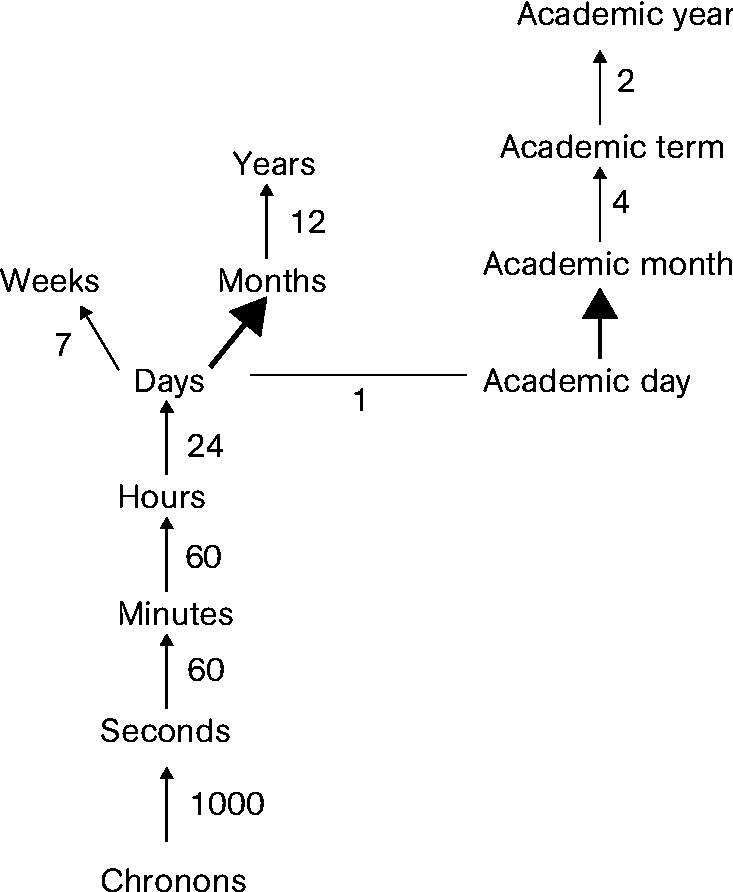
\includegraphics[scale=0.5]{graphs/granularityGraph.pdf}
%\caption{A granularity graph example}
%\label{fig:granularity-graph-example}
%\end{figure}


Next, in subsection \ref{subsec:timedomain-calendar}, some basic concepts and issues concerning calendars are explained.

\subsection{Calendars}
\label{subsec:timedomain-calendar}
%maybe introduce previously the concept of time units, linear hierarchy and time point.

This subsection will concern \emph{calendars}. A calendar provides some sort of human interpretation of time. As such, calendars provide meaning or interpretation to temporal values where this meaning or interpretation is relevant or useful to the user. More precisely, calendars determine the mapping between human-meaningful time values and an underlying time model~\cite{Dyreson1994}. More formally, a calendar is an organization of different granularities (e.g. granularities day, month and year) in a hierarchy. In order to formally define what a calendar is, some other concepts should first be introduced~\cite{Kraus1997}:


%\begin{svgraybox}
%\vspace{-10pt}
%\begin{definition}\textbf{(Calendar)}\\
%A \emph{\textbf{calendar}} 
%\end{definition}
%\vspace{-10pt}
%\end{svgraybox}


\begin{svgraybox}
\vspace{-10pt}
\begin{definition}\textbf{Linear Hierarchy of Granularities}\\
A \emph{\textbf{linear hierarchy of granularities}} is a finite set of granularities with a linear order (denoted $\sqsubset$). The most coarse granularity is called \emph{the top of the hierarchy} and must be an infinite set while all other granularities must be finite sets.
\end{definition}
\vspace{-10pt}
\end{svgraybox}

An example of a linear hierarchy is the set $\left\{ \text{days, months, years} \right\}$, where days $\sqsubset$ months and months $\sqsubset$ years. With this, a \emph{linear calendar} can be defined.

\begin{svgraybox}
\vspace{-10pt}
\begin{definition}\textbf{Linear Calendar}\\
A \emph{\textbf{linear calendar}} consist of a linear hierarchy of granularities and a validity predicate which specifies if a granule is valid in the calendar.
\end{definition}
\vspace{-10pt}
\end{svgraybox}

An example of a linear calendar could be the linear hierarchy $\left\{ \text{days, months, years} \right\}$, where days $\sqsubset$ months and months $\sqsubset$ years, together with a validity predicate that excludes time indications like `32 april 2012' or `30 february 2012'.

%The linear hierarchy days $\sqsubset$ months $\sqsubset$ years represents a linear calendar. It is necessary to define the validity predicates because 17 January 2012 is a valid element of the calendar whereas 30 February 2012 is not.
 
\textcolor{red}{CHECK}
\subsubsection{\label{subsubsubsec:julian-day-number}An example of temporal domain: Julian Day Number}
% proposal for the underlying Julian Day Number domain.

The Julian Day number \emph{JDN} \cite{Dir96} is a counter. Its value is incremented in one unit every day from 1 January 4713 B.C. at 12:00 noon. The particularity of starting at noon was useful for astronomers: the observations they took one night belonged to the same Julian Day.\\
Note that the Julian Day represents whole days. There is an extension that allows to represent any precision needed (it is called Julian Date). By default, a Julian Day is expressed in Universal Time. (U.T, also known as Solar Time). However, there are representations in Terrestrial Time (T.T), Epheris Time (J.E.D. or J.D.E.). Any time scale different from Universal Time must be explicited after the Julian Day number. There are several conversion formulas~\cite{Usn}\cite{Wik}\cite{Lea} between a date in Gregorian calendar  format and a date in  JDN format. The inverse conversion formula is proposed in~\cite{Fliegel:1968:LEM:364096.364097}\\

There are many alternatives to optimize the representation of Julian Day numbers because of its extremely far origin (4713 B.C. year). Table \ref{table:juliandayrepresentations} shows several time domains that can be calculated from the Julian Date, some of them are proposed just for optimization purposes.


\begin{table}
\caption{Julian Day representations}
\label{table:juliandayrepresentations}

\begin{tabular}{p{2cm}p{4cm}p{4cm}p{2cm}}
%header ------------------------------------------------------
\hline\noalign{\smallskip}
Name & From & Formula & Current Value  \\ 
\noalign{\smallskip}\svhline\noalign{\smallskip}
%header ------------------------------------------------------
Julian Date (JD)$^a$ & 12:00 noon Monday 1 January 4713 B.C & & 2455278. 85488  \\ 
Julian Day Number (JDN)$^b$ & 12:00 noon  Monday 1 January 4713 B.C. & JND = floor(JD) & 2455278 \\ 
Reduced Julian Day (RJD)$^c$ & 12:00 noon Tuesday 16 November 1858 A.C. & RJD = JD - 2400000 & 55278.85488  \\ 
Modified Julian Day (MJD)$^d$ & 00:00 Wednesday 17 November 1858 A.C. & MJD = JD - 2400000,5 & 55278.35488 \\ 
Truncated Julian Day (TJD)$^e$ & 00:00 Friday 24 May 1968 A.C. & TJD = JD - 2440000,5 & 15278.35488  \\ 
Truncated Julian Day (TJD)$^f$ & 00:00 Thursday 10 November 1995 A.C. & TJD = (JD- 0,5) mod 10000 & 5278. 35488   \\ 
Dublin Julian Day (DJD))$^g$ & 12:00 noon Sunday 31 December 1899 A.C. & DJD = JD - 2415020 & 40258. 85488 \\ 
Chronological Julian Day (CJD)$^h$  & 00:00 Monday 1 January 4713 B.C. & CJD = JD + 0,5 + timezone adjust. & 2455279. 3548843 (UT)  \\ 
Lilian Day Number$^i$ & Friday 15 October 1582 & floor(JD-2299160,5) & 156118 \\ 
ANSI Date$^j$  & Monday 1 January 1601 & floor(JD-2305812,5) & 149466  \\ 
Rata die$^k$  & Monday 1 January 1 A.C & floor(JD - 1721424.5) & 733854 \\ 
Unix time$^l$  & Thursday 1 January 1970 A.C. & (JD – 2440587.5) × 86400 & 1269333062 \\ 
\noalign{\smallskip}\hline\noalign{\smallskip}
\end{tabular}
$^a$ This is an extension of the Julian Day that allows time representation. \\
$^b$  Each day changes at noon. \\
$^c$  Used by astronomers. \\
$^d$ It starts at midnight. \\
$^e$ Definition from NASA. \cite{Sch}. \\
$^f$ Definition from NIST. \cite{Nis}. \\
$g$ Introduced by the IAU in 1995. \\
$^h$ The timezone must be explicited. Each day changes at midnight. \\
$^i$ The number of days since Gregorian calendar in Universal Time. \\
$^j$ The origin for COBOL integer dates. \\
$^k$  The number of days since actual era. \\
$^l$  It counts the seconds not the day. \\
\end{table}

\textcolor{red}{END CHECK}

The next section briefly introduces temporal relationships.

\subsection{Temporal Relationships}
%an explanation on allen's temporal relations.
%definition of fuzzy temporal interval
In this section, a brief introduction can be found, concerning \emph{temporal relationships}, sometimes also called `temporal relations'\cite{Billiet:Pons:Matthe:DeTre:Pons:2011:BipolarFuzzy}. Temporal relationships can be seen as relationships between temporal elements or instants.

\def\JPicScale{0.5}
\begin{figure}[h]
\centering
%%Created by jPicEdt 1.4.1_03: mixed JPIC-XML/LaTeX format
%%Tue Jan 17 09:05:12 CET 2012
%%Begin JPIC-XML
%<?xml version="1.0" standalone="yes"?>
%<jpic x-min="4" x-max="85" y-min="-2" y-max="140" auto-bounding="true">
%<text text-vert-align= "center-v"
%	 anchor-point= "(4,70)"
%	 fill-style= "none"
%	 text-frame= "noframe"
%	 text-hor-align= "center-h"
%	 >
%I Before J
%</text>
%<multicurve fill-style= "none"
%	 points= "(50,75);(50,75);(80,75);(80,75)"
%	 />
%<multicurve fill-style= "none"
%	 points= "(25,65);(25,65);(45,65);(45,65)"
%	 />
%<text text-vert-align= "center-v"
%	 anchor-point= "(35,67.5)"
%	 fill-style= "none"
%	 text-frame= "noframe"
%	 text-hor-align= "center-h"
%	 >
%I
%</text>
%<text text-vert-align= "center-v"
%	 anchor-point= "(65,77.5)"
%	 fill-style= "none"
%	 text-frame= "noframe"
%	 text-hor-align= "center-h"
%	 >
%J
%</text>
%<text text-vert-align= "center-v"
%	 anchor-point= "(4,56)"
%	 fill-style= "none"
%	 text-frame= "noframe"
%	 text-hor-align= "center-h"
%	 >
%I Equal J
%</text>
%<text text-vert-align= "center-v"
%	 anchor-point= "(20,140)"
%	 fill-style= "none"
%	 text-frame= "noframe"
%	 text-hor-align= "center-h"
%	 >
%
%</text>
%<multicurve fill-style= "none"
%	 points= "(20,85);(20,85);(20,0);(20,0)"
%	 />
%<multicurve right-arrow= "head"
%	 fill-style= "none"
%	 points= "(20,0);(20,0);(85,0);(85,0)"
%	 />
%<text text-vert-align= "center-v"
%	 anchor-point= "(80,-2)"
%	 fill-style= "none"
%	 text-frame= "noframe"
%	 text-hor-align= "center-h"
%	 >
%Time
%</text>
%<multicurve fill-style= "none"
%	 points= "(25,55);(25,55);(45,55);(45,55)"
%	 />
%<text text-vert-align= "center-v"
%	 anchor-point= "(35,57.5)"
%	 fill-style= "none"
%	 text-frame= "noframe"
%	 text-hor-align= "center-h"
%	 >
%J
%</text>
%<text text-vert-align= "center-v"
%	 anchor-point= "(4,46)"
%	 fill-style= "none"
%	 text-frame= "noframe"
%	 text-hor-align= "center-h"
%	 >
%I Meets J
%</text>
%<text text-vert-align= "center-v"
%	 anchor-point= "(40,40)"
%	 fill-style= "none"
%	 text-frame= "noframe"
%	 text-hor-align= "center-h"
%	 >
%
%</text>
%<multicurve fill-style= "none"
%	 points= "(45,45);(45,45);(65,45);(65,45)"
%	 />
%<text text-vert-align= "center-v"
%	 anchor-point= "(55,47.5)"
%	 fill-style= "none"
%	 text-frame= "noframe"
%	 text-hor-align= "center-h"
%	 >
%J
%</text>
%<text text-vert-align= "center-v"
%	 anchor-point= "(6,36)"
%	 fill-style= "none"
%	 text-frame= "noframe"
%	 text-hor-align= "center-h"
%	 >
%I Overlaps J
%</text>
%<multicurve fill-style= "none"
%	 points= "(30,35);(30,35);(50,35);(50,35)"
%	 />
%<text text-vert-align= "center-v"
%	 anchor-point= "(40,37.5)"
%	 fill-style= "none"
%	 text-frame= "noframe"
%	 text-hor-align= "center-h"
%	 >
%J
%</text>
%<text text-vert-align= "center-v"
%	 anchor-point= "(4,26)"
%	 fill-style= "none"
%	 text-frame= "noframe"
%	 text-hor-align= "center-h"
%	 >
%I During J
%</text>
%<multicurve fill-style= "none"
%	 points= "(20,25);(20,25);(50,25);(50,25)"
%	 />
%<text text-vert-align= "center-v"
%	 anchor-point= "(35,27.5)"
%	 fill-style= "none"
%	 text-frame= "noframe"
%	 text-hor-align= "center-h"
%	 >
%J
%</text>
%<text text-vert-align= "center-v"
%	 anchor-point= "(4,16)"
%	 fill-style= "none"
%	 text-frame= "noframe"
%	 text-hor-align= "center-h"
%	 >
%I Starts J
%</text>
%<multicurve fill-style= "none"
%	 points= "(25,15);(25,15);(55,15);(55,15)"
%	 />
%<text text-vert-align= "center-v"
%	 anchor-point= "(6,6)"
%	 fill-style= "none"
%	 text-frame= "noframe"
%	 text-hor-align= "center-h"
%	 >
%I Finishes J
%</text>
%<text text-vert-align= "center-v"
%	 anchor-point= "(35,17.5)"
%	 fill-style= "none"
%	 text-frame= "noframe"
%	 text-hor-align= "center-h"
%	 >
%J
%</text>
%<text text-vert-align= "center-v"
%	 anchor-point= "(35,7.5)"
%	 fill-style= "none"
%	 text-frame= "noframe"
%	 text-hor-align= "center-h"
%	 >
%J
%</text>
%<multicurve fill-style= "none"
%	 points= "(25,5);(25,5);(45,5);(45,5)"
%	 />
%<text text-vert-align= "center-v"
%	 anchor-point= "(6,80)"
%	 fill-style= "none"
%	 text-frame= "noframe"
%	 text-hor-align= "center-h"
%	 >
%Relations
%</text>
%</jpic>
%%End JPIC-XML
%LaTeX-picture environment using emulated lines and arcs
%You can rescale the whole picture (to 80% for instance) by using the command \def\JPicScale{0.8}
\ifx\JPicScale\undefined\def\JPicScale{1}\fi
\unitlength \JPicScale mm
\begin{picture}(85,140)(0,0)
\put(4,70){\makebox(0,0)[cc]{I Before J}}

\linethickness{0.3mm}
\put(50,75){\line(1,0){30}}
\linethickness{0.3mm}
\put(25,65){\line(1,0){20}}
\put(35,67.5){\makebox(0,0)[cc]{I}}

\put(65,77.5){\makebox(0,0)[cc]{J}}

\put(4,56){\makebox(0,0)[cc]{I Equal J}}

\put(20,140){\makebox(0,0)[cc]{}}

\linethickness{0.3mm}
\put(20,0){\line(0,1){85}}
\linethickness{0.3mm}
\put(20,0){\line(1,0){65}}
\put(85,0){\vector(1,0){0.12}}
\put(80,-2){\makebox(0,0)[cc]{Time}}

\linethickness{0.3mm}
\put(25,55){\line(1,0){20}}
\put(35,57.5){\makebox(0,0)[cc]{J}}

\put(4,46){\makebox(0,0)[cc]{I Meets J}}

\put(40,40){\makebox(0,0)[cc]{}}

\linethickness{0.3mm}
\put(45,45){\line(1,0){20}}
\put(55,47.5){\makebox(0,0)[cc]{J}}

\put(6,36){\makebox(0,0)[cc]{I Overlaps J}}

\linethickness{0.3mm}
\put(30,35){\line(1,0){20}}
\put(40,37.5){\makebox(0,0)[cc]{J}}

\put(4,26){\makebox(0,0)[cc]{I During J}}

\linethickness{0.3mm}
\put(20,25){\line(1,0){30}}
\put(35,27.5){\makebox(0,0)[cc]{J}}

\put(4,16){\makebox(0,0)[cc]{I Starts J}}

\linethickness{0.3mm}
\put(25,15){\line(1,0){30}}
\put(6,6){\makebox(0,0)[cc]{I Finishes J}}

\put(35,17.5){\makebox(0,0)[cc]{J}}

\put(35,7.5){\makebox(0,0)[cc]{J}}

\linethickness{0.3mm}
\put(25,5){\line(1,0){20}}
\put(6,80){\makebox(0,0)[cc]{Relations}}

\end{picture}

\caption{Allen relations between two time intervals.}
\label{fig:allen}
\end{figure}

Several operators are defined in order to compare temporal elements or time points. Allen~\cite{Allen83} first described the relationships between time intervals and as a special case, between time points. Figure \ref{fig:allen} shows the temporal relationships Allen discerned. Some proposals can be applied to both crisp and fuzzy temporal intervals~\cite{ohlbach2004},~\cite{nagypal2003},~\cite{schockaert08}. 

\textcolor{red}{MOVE TO FUZZY PART}
For this fuzzy comparisons~\cite{garrido2009} proposed some different temporal relations that can be easily implemented by means of regular fuzzy operations.
\textcolor{red}{END MOVE TO FUZZY PART}

In the next section, some basic concepts and terminology about temporal databases are presented, followed by an overview of some interesting issues concerning temporal databases and a survey of some commercial temporal database systems.
\def\JPicScale{1}
\section{Temporal Databases}
\label{sec:temporal-databases}
%
% Temporal databases
%
A temporal database can generally be seen as a database that manages some temporal aspects in its schema~\cite{etzion1998},~\cite{Billiet:Pons:Matthe:DeTre:Pons:2011:BipolarFuzzy}. In subsection~\ref{subsec:td-general-concepts}, some main concepts and properties concerning temporal databases and their definitions are presented and explained. In subsections~\ref{subsubsec:primary-key} and~\ref{subsubsec:consistency}, some main issues of relational temporal databases are presented and discussed. Finally, subsection~\ref{Comm-temp} presents an overview of some commercial temporal database systems.

\subsection{\label{subsec:td-general-concepts}Basic Concepts and Properties}
A database schema models some part of reality. As mentioned in the introduction, the part of reality a temporal database schema tries to model, contains some temporal aspects. For example, in this part of reality, some concepts or objects could have time-related or time-variant properties. The modelling of these temporal aspects has to be handled specifically in order for the database to maintain a consistent model of reality.

Thus, a temporal database will contain \emph{temporal values}, i.e. values representing (indications of) time. Temporal values in a temporal database can be classified into the following types based on their interpretation and modelling purpose. The definitions and explanations of these types can be found in~\cite{Dyreson1994} and~\cite{Nascimento95decisiontime} and more information can be found in~\cite{Jensen:1991:IIM:627283.627484},~\cite{Snodgrass:1984:TQL:588011.588041} and~\cite{Nascimento95decisiontime}.

\begin{svgraybox}
\vspace{-10pt}
\begin{definition}\textbf{Valid Time}~\cite{Dyreson1994}\\
The \emph{\textbf{valid-time}} (VT) of a fact is the time when the fact is true in the modeled reality.
\end{definition}

\begin{definition}\textbf{Transaction Time}~\cite{Dyreson1994}\\
A database fact is stored in a database at some point in time, and after it is stored, it is current until logically deleted. The \emph{\textbf{transaction-time}} (TT) of a database fact is the time when the fact is current in the database and may be retrieved.
\end{definition}

\begin{definition}\textbf{Decision Time}~\cite{Nascimento95decisiontime}\\
\emph{\textbf{Decision time}} (DT) denotes the time when an event was decided to happen.
\end{definition}

\begin{definition}\textbf{User-defined Time}~\cite{Dyreson1994}\\
\emph{\textbf{User-defined time}} (UDT) is an uninterpreted attribute domain of date and time.
\end{definition}
\vspace{-10pt}
\end{svgraybox}

\emph{Valid times} are usually provided by the user, whereas \emph{transaction-times} are usually system-generated and -supplied~\cite{Dyreson1994}. Temporal values of type UDT are not given any extraordinary interpretation and have thus no extraordinary query language support~\cite{Dyreson1994}.

A \emph{temporal database} can now formally be defined as follows:

\begin{svgraybox}
\vspace{-10pt}
\begin{definition}\textbf{Temporal Database}~\cite{Dyreson1994}\\
A \emph{\textbf{temporal database}} supports some aspect of time, not counting user-defined time.
\end{definition}
\vspace{-10pt}
\end{svgraybox}

In a relational temporal database, temporal values will of course be in the tuples of the extensions of temporal relations:

\begin{svgraybox}
\vspace{-10pt}
\begin{definition}\textbf{Valid-time Relation}~\cite{Dyreson1994}\\
A \emph{\textbf{valid-time relation}} is a relation with exactly one system supported valid-time.
\end{definition}

\begin{definition}\textbf{Transaction-time Relation}~\cite{Dyreson1994}\\
A \emph{\textbf{transaction-time relation}} is a relation with exactly one system supported transaction-time.
\end{definition}
\vspace{-10pt}
\end{svgraybox}

A \emph{valid-time}, respectively \emph{transaction-time} \emph{relational database} is now defined as containing one or more valid-time, respectively transaction-time relations~\cite{Dyreson1994}. Next to this, \emph{bitemporal} relational databases contain both valid-time and transaction-time~\cite{Dyreson1994} and tritemporal databases contain valid-time, transaction-time and decision-time~\cite{Nascimento95decisiontime}.


%Database models can also be classified into \emph{bi-temporal} (both valid and transaction-time) or \emph{tri-temporal}  (bi-temporal and decision-time) models.


A very extensive list of the most well-known temporal database models can be found in ~\cite{Yu1998}. As it is of course necessary to define a consistent way to query the temporal data, there are several proposals concerned with query languages and query language adaptations for temporal databases like ~\cite{TSQL} and ~\cite{Snodgrass98}.




%A \emph{temporal database}~\cite{etzion1998} is a database that manages some aspects of time in its schema~\cite{Dyreson1994}. The reality a temporal database tries to model, contains some temporal notions which have to be handled specifically in order to maintain a consistent modelling behavior. A very extensive list with the most well-known models in temporal databases can be found in ~\cite{Yu1998}. Nevertheless, it is necessary to define some consistent way to query the temporal data. There are several languages for querying temporal databases like TSQL~\cite{TSQL}. In~\cite{Snodgrass98} a proposal to add temporal support to the standard SQL is given.


%\begin{svgraybox}
%The temporal notions in temporal databases can be classified into the following types based on their interpretation and modelling purpose. User-defined time has no interpretation, but the other types do:\\

%	\textbf{Transaction time} \emph{TT}~\cite{Jensen:1991:IIM:627283.627484}: The time when the fact is stored in the database.\\
	
%	\textbf{Valid time} \emph{VT}~\cite{Snodgrass:1984:TQL:588011.588041}: The time when the fact is true in the modelled reality.\\
	
%	\textbf{Decision time} \emph{DT}~\cite{Nascimento95}: The time when an event was decided to happen. \\
%\end{svgraybox}
	


%In the following sections, some of the main points of attention concerning relational temporal databases are explained and discussed.

In the rest of the chapter, the focus will be on concepts and issues concerning valid-time relations and aspects of valid-time relations. For this reason, the next two sections will present and discuss some main issues concerning temporal databases, specifically applied to or presented in the context of valid-time relations.

\subsection{\label{subsubsec:primary-key}Primary Keys in Valid-time Relation Design}
Generally, when designing a relation based on a relational database model, a subset of the relation's attribute set is usually chosen as primary key. The values of a tuple for these attributes will then uniquely determine this tuple, hence no two distinct tuples may have the exact same values for every attribute in this primary key. Next to attributes unrelated to time, a valid-time relation schema will typically contain one or more attributes which model the valid-time aspects and behavior of the real objects and concepts modelled by the relation schema. In this work, these attributes are called \emph{valid-time attributes}. In valid-time relation extensions, distinct tuples can exist containing the exact same values for every attribute except the valid-time attributes. These distinct tuples represent distinct versions of the same real object or concept, valid during different time periods. To allow the existence of such tuples when designing a valid-time relation using a relational database model, the most common solution is to include the valid-time attributes in the primary key.
%One of the first tasks in the design of a database is the choice for the primary key. In a temporal database, the most common solution for the choice of the primary key is to extend the primary key with the temporal value. Nevertheless, when dealing with uncertainty in the temporal values, the solution is usually to create a version identifier otherwise the primary key have uncertainty which should be avoided.

The following example illustrates this primary key issue.

\begin{example}
\label{ex:pk}
Consider the example valid-time relation visualized in table~\ref{table:example-database}, which models when certain people worked as employees in a certain company and under whose supervision they worked during that time. The valid-time attributes `Start' and `End' describe the year when an employee started, respectively finished working for the company. For example, the last tuple visualized in table~\ref{table:example-database} represents that the employee represented by this tuple started working for the company in 2005 and finished in 2009. The attributes `Name', `Birthday' and `Supervisor' describe respectively the name, birthday date and unique identifier of the supervisor of an employee in the time during which he or she worked for the company. When correct, the date of an employee's birthday never changes and as such, the modelling of birthday dates has no effect on the database consistency. The `Birthday' attribute thus describes UDT values. The attribute `ID' describes employee identifiers. For each tuple, this identifier (a number) uniquely identifies the employee represented by the tuple. 

Now consider $\{$ID$\}$ being the primary key and consider the company wanting to hire Sarah again in 2010. This would be represented by another tuple in the relation, containing value 4 for attribute `ID'. The existence of such a tuple is of course not allowed by the primary key, because it would mean the existence of two distinct tuples containing value 4 for attribute `ID'. This problem can now be solved by defining a new primary key: $\{$ID, Start, End$\}$, which allows for the existence of distinct tuples with value 4 for attribute `ID', as long as they have different values for attributes `Start' or `End'. The resulting relation is shown in table~\ref{table:example-database-with-new-pk}.
%Consider the example database visualized in table \ref{table:example-database}. It contains data representing employees in a company, and two temporal values which represent a valid-time interval. Consider now that we want to hire Sarah again. That is not possible because of the primary key (ID) does not allow to insert again the row Sarah but with a different start and end time. In some models this is resolved by adding to the primary key both values Start and End years. The resulting database allows to insert a new row where Sarah the year 2010. But this modification also allows to insert spurious values e.g., inconsistent time periods (see last row in table \ref{table:example-database-with-new-pk}).

\end{example}
%\begin{note}
%The attribute `Age' in the presented relations visualized in tables~\ref{table:example-database},~\ref{table:example-database-with-new-pk} and~\ref{table:example-database-update} describes the age of an employee and is included as an example of . In reality, the birthday of the employee should be stored in the database, rather than the age, because the age 
%In the presented relations visualized in tables~\ref{table:example-database},~\ref{table:example-database-with-new-pk} and~\ref{table:example-database-update}, the value of a tuple for attribute `Supervisor' should actually contain the unique identifier of the supervisor of the employee represented by the tuple. the relation `Supervisor' stores the ID of the employee. To improve the readability of the example, the tables show the name of the employee. Note also that the field for the age is expressed as the age in years whereas the value stored in the database is the birthday.
%\end{note}



%Extending a primary key to include temporal attributes allows for the insertion of spurious values, for example representing temporal inconsistencies. This is shown in table \ref{table:example-database-with-new-pk}, where it seems Sarah was rehired in 2007 and fired in 2008.

%\vspace{-10pt}

\begin{table}
\centering
\caption{Example relation modelling the employees of a company. Values for the `Birthday' attribute are visualized here in `dd/mm/yyyy' format.}
\begin{tabular}{c c c c c c }
\hline
\textbf{ID} & \textbf{Name} & \textbf{Birthday} & \textbf{Supervisor} & \textbf{Start} & \textbf{End} \\ \hline
1 & Peter & 24/10/1985 & 3 &  2010 & - \\
2 & Maria & 03/04/1984 & 3 & 2001 & - \\
3 & John & 21/02/1964 & - &  1999 & - \\
4 & Sarah & 29/11/1985 & 2 &  2005 & 2009 \\
\hline 
\end{tabular}
\label{table:example-database}

%\vspace{10pt}


\end{table}

%\vspace{-25pt}


%\vspace{-10pt}

\begin{table}
\centering
\caption{Example relation after including the valid-time attributes in the primary key and adding a tuple.}
\begin{tabular}{c c c c c c }
\hline
\textbf{ID} & \textbf{Name} & \textbf{Birthday} & \textbf{Supervisor} & \textbf{Start} & \textbf{End} \\ \hline
1 & Peter & 24/10/1985 & 3 &  2010 & - \\
2 & Maria & 03/04/1984 & 3 & 2001 & - \\
3 & John & 21/02/1964 & - &  1999 & - \\
4 & Sarah & 29/11/1985 & 2 &  2005 & 2009 \\
4 & Sarah & 29/11/1985 & 2 &  2010 & - \\
%4 & Sarah & 29/11/1985 & 2 &  2007 & 2008 \\
\hline 
\end{tabular}
\label{table:example-database-with-new-pk}
\end{table}

%The next subsection is concerned with another interresting issue.

\subsection{\label{subsubsec:consistency}Consistency in Valid-time Relation Content Modification}
The solution presented in subsection~\ref{subsubsec:primary-key} concerns relation design and consists of including the valid-time attributes in the primary key. Unfortunately, implementing this solution as such allows for the existence of records whose values imply inconsistencies with respect to the modelling of reality.

Consider a valid-time relation of which the primary key can be partitioned into two sets of attributes. One set contains attributes totally unrelated to time, for which the values of a record allow to uniquely identify the object or concept represented by the record. The other set contains the valid-time attribute(s). Because the valid-time attribute(s) is(are) included in the primary key, the existence of distinct records with exactly the same values for all time-unrelated attributes and distinct values for at least one valid-time attribute is not prohibited. Thus, inserting such records into the relation is not prohibited either, even if the information represented by the values for the valid-time attributes shows clear inconsistencies. An example.

\begin{example}
\label{ex:prob}
Consider the example valid-time relation visualized in table~\ref{table:erconsistency}, which is based on the relation visualized in table~\ref{table:example-database}. The primary key is again $\{$ID, Start, End$\}$. The last record in the relation represents a person named `Sarah' started working for the company in 2007 and finished in 2008, with supervisor `John'. However, the fourth record represents the same person (the value for attribute `ID' is the same) started working for the company in 2005 and finished in 2009, with supervisor `Maria'. The intention is clear: Sarah worked in the company from 2005 to 2009, first for Maria, then for John, then again for Maria. It is of course possible for an employee to change supervisors, but it is of course impossible for a person to start working in the same company twice at different times, for different supervisors, without stopping to work for one in between, as it is impossible to stop working for a supervisor twice at different times, without working for another one in between. The valid-time information represented by the last record is clearly not consistent with the valid-time information represented by the fourth record, or vice versa.
\end{example}

\begin{table}
\centering
\caption{Example relation with records whose values for the valid-time attributes violate consistency.}
\begin{tabular}{c c c c c c }
\hline
\textbf{ID} & \textbf{Name} & \textbf{Birthday} & \textbf{Supervisor} & \textbf{Start} & \textbf{End} \\ \hline
1 & Peter & 24/10/1985 & 3 &  2010 & - \\
2 & Maria & 03/04/1984 & 3 & 2001 & - \\
3 & John & 21/02/1964 & - &  1999 & - \\
4 & Sarah & 29/11/1985 & 2 &  2005 & 2009 \\
%4 & Sarah & 29/11/1985 & 2 &  2010 & - \\
4 & Sarah & 29/11/1985 & 3 &  2007 & 2008 \\
\hline 
\end{tabular}
\label{table:erconsistency}
\end{table}

The most usual approach to deal with this inconsistency problem is to adapt the DML used by the DBMS, as to enforce consistency towards time with respect to the modelled reality.

\begin{example}
Consider the problem presented in example~\ref{ex:prob}. The inconsistency arises when the last record in table~\ref{table:erconsistency} is inserted. Because the record's values for the valid-time attributes differ from those of the fourth record, the last record is accepted. The DML statement used was (the table is called `Employees'):

\begin{verbatim}
INSERT INTO Employees VALUES
 (4, `Sarah', `29/11/1985', 3, 2007, 2008);
\end{verbatim}

\noindent
The inconsistency problem can now be solved by replacing this statement with:

\begin{verbatim}
UPDATE Employees SET `End' = `2007' WHERE
 (ID = 4) AND (Start = 2005) AND (End = 2009);
INSERT INTO Employees VALUES
 (4, `Sarah', `29/11/1985', 3, 2007, 2008);
INSERT INTO Employees VALUES
 (4, `Sarah', `29/11/1985', 2, 2008, 2009);
\end{verbatim}

\noindent
The resulting relation is visualized in table~\ref{table:example-database-update}.

\end{example}

%As stated in subsection \ref{subsubsec:primary-key}, one of the main issues concerns the insertion of spurious values in a relation. Another issue concerns the possible breach of consistency when updating records. The most usual approach to deal with this is to change the database DML to enforce the consistency with which the temporal relation models the temporal properties of the part of reality the relation models. An example of such DML adaptation is given below.

%The consistence mechanism in a temporal database is usually re-defined. The main problem is the insertion of spurious values in the database, as shown in example \ref{ex:pk}, in table \ref{table:example-database-with-new-pk}. The most usual solution is to re-define the DML (\emph{Data Manipulation Language}). e.g., the \emph{update} sentence is redefined as two sentences an update and a create sentence as illustrated in the following example.

%\begin{example}
%Consider the database in table \ref{table:example-database}. The employee with ID=3 (John) works now for the employee with ID= 4 (Sarah). The update is made in the following sentence:

%The following \emph{update} sentence:

%\begin{verbatim}
%Update Employees set 'Works for' = 4 where ID=3;
%\end{verbatim}

%Is translated into the following two sentences: an update for the last version of the row and an insert sentence for the new version. Consider that the time in the  system is the year 2010. Then, the update sentence showed above is translated into:

%\begin{verbatim}
%Update Employees set EndYear = 2010 where ID=3;
%Insert into Employees values (3,John,52,Sarah,2010,-);
%\end{verbatim}

\begin{table}
\centering
\caption{Example relation updated maintaining consistency.}
\begin{tabular}{c c c c c c }
\hline
\textbf{ID} & \textbf{Name} & \textbf{Birthday} & \textbf{Supervisor} & \textbf{Start} & \textbf{End} \\ \hline
1 & Peter & 24/10/1985 & 3 &  2010 & - \\
2 & Maria & 03/04/1984 & - & 2001 & - \\
3 & John & 21/02/1964 & - &  1999 & 2010 \\
3 & John & 21/02/1964 & - &  2010 & - \\
4 & Sarah & 29/11/1985 & 2 &  2005 & 2007 \\
4 & Sarah & 29/11/1985 & 3 &  2007 & 2008 \\
4 & Sarah & 29/11/1985 & 2 &  2008 & 2009 \\
\hline 
\end{tabular}
\label{table:example-database-update}

%\vspace{10pt}


\end{table}

%\vspace{-25pt}

%Table \ref{table:example-database-update} shows the resulting database after the update sentence.

%\end{example}


\subsection{\label{Comm-temp}Commercial Temporal Database Systems}
Several commercial temporal DBMS exist. Table~\ref{table:commercial-temporal-db} gives an overview of some of the more well-known temporal DBMS and provides references for more information. 

Oracle workspace manager~\cite{oracle2009} and TimeDB~\cite{timedb2005} are libraries for dealing with time in OracleDB. On another note, TimeDB and Postgree Temporal~\cite{posgree2009} are similar: both are simple implementations that implement a subset of the Allen operators and some operations for the creation and manipulation of temporal attributes (valid-time, transaction-time or both times are supported). Teradata~\cite{teradata2011} is mainly a business intelligence system designed for data mining. Secondo~\cite{Dieker2000} is an extensible database system in which the core of the database may be replaced by a customized algebra. It is designed for non-standard applications and it supports both valid and transaction-times. 

 The most complete implementation is Workspace Manager.

Unfortunately, none of these systems take data imperfections into account, neither in data storage nor in querying.

\begin{table}
\centering
\caption{Commercial Temporal Database Systems. }
\begin{tabular}{c c c c c c }
\hline
\textbf{Name} & \textbf{Time Supported} & \textbf{Comments} & \textbf{Reference}  \\ \hline
Oracle Workspace Manager & VT and TT. & Package for Oracle DB. & \cite{oracle2009}\\
TimeDB & VT and TT. & Interface for Oracle DB. & \cite{timedb2005}\\
Postgree Temporal & VT. & Package for Postgree SQL. & \cite{posgree2009}\\
Teradata & VT and TT. & Used for data-mining. & \cite{teradata2011}\\
Secondo & VT and TT. & Spatio-temporal database. & \cite{Guting} \\
\hline 
\end{tabular}
\label{table:commercial-temporal-db}

%\vspace{10pt}


\end{table}

%\subsubsection{Oracle Workspace Manager}
%
%\begin{figure}
%\centering
%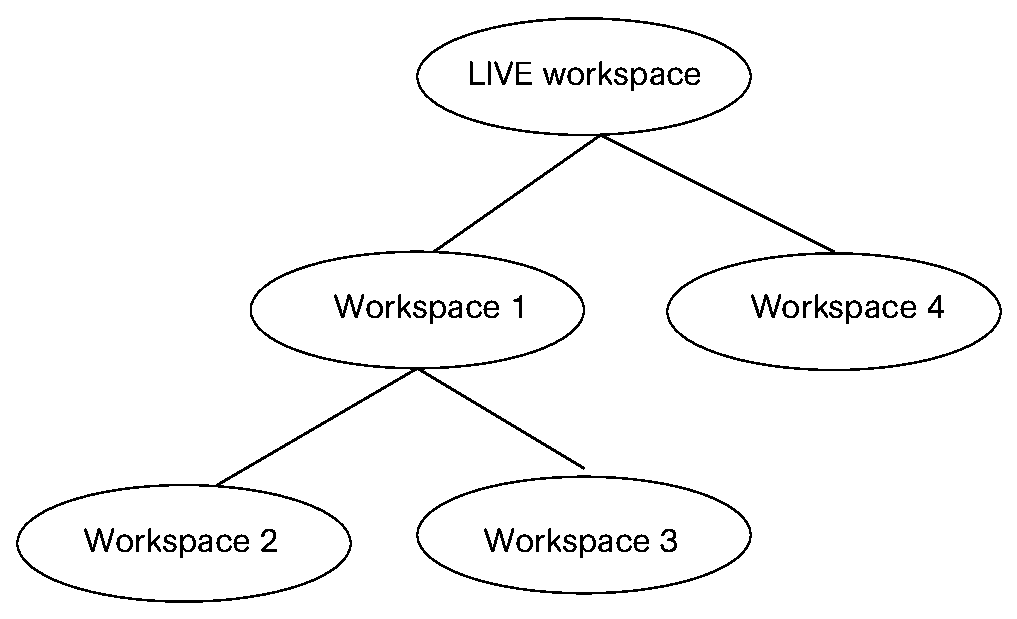
\includegraphics[scale=0.5]{graphs/workspaceTopology.eps}
%\caption{A sample topology in the workspace manager.}
%\label{fig:workspace-topology}
%\end{figure}
%
%Oracle workspace manager \cite{OraE118602} package allows to get several versions of the data in the same database. It is also possible to version only a table. The main benefits of this are two:
%
%\begin{itemize}
%\item
%Organization and optimization of data in a hierarchical frames: It is possible to create a frame of time (a workspace) and work only with that partial version of the data. It is provided a mechanism to merge data among different workspaces and to solve conflicts. The organization of data in these workspaces for very large tables result in smaller time access.
%\item
%Valid time as well as transaction-time are managed by the system. Each update sentence makes a change in the versioning of a row.
%\end{itemize}
%
%When a table is versioned, the system creates a few tables and views as well as auxiliary structures to allow keep several version of the data, while keeping the primary key defined by the user.
%
%A workspace is a logical group of a set of changes (versions of tuples) and allows consistent access, thus the user always obtain the correct data version. Workspaces are ordered in a hierarchy. The top level is called LIVE workspace (see figure \ref{fig:workspace-topology}).  \\
%
%The system only makes a copy of a tuple if it is changed. In order to access different versions of the tuple, the context must be changed. Also, it is not necessarily to modify the SQL code to access to versioned tables.\\
%%When a table is versioned, it is renamed as table\_LT. Here is stored all the data for the information together metadata for the versioning. An auxiliary table is created with the workspace metadata with the name table\_AUX. A view is created with the name of the original table to allow querying without versioning.


\def\JPicScale{1}
\section{Imprecision, Uncertainty and Vagueness in Temporal Databases}
\label{sec:imprecision-uncertainty}
%
% Fuzzy temporal databases
%
Consider a logistics company which transports packages. The time when a package would arrive at its destination may be estimated and can eventually be researched, but it is typically not always precisely known. For such companies and in many other situations, information systems able to handle imperfection corresponding to certain temporal aspects of the objects modelled by the system are necessary. The transition between granularities~\cite{Lin97} is also sometimes considered as a source of imprecision. Therefore, some proposals consider granularity as the base of the temporal model~\cite{Cru97}.
%Some software applications deal with uncertainty related to time. e.g. a logistics company which transports packages from one destination to another. The time when the package would be at the end point may be estimated but not precisely known. These applications need to manage the uncertainty with respect to the temporal attributes of the objects stored in the database.

Data imperfection is usually the focus of research in fuzzy databases. In fuzzy databases~\cite{Galindo2006}, uncertainty is usually expected to appear at storage level whereas imprecision is usually expected to appear in querying. Concerning temporal databases, there are several approaches to handle uncertainty in temporal data stored in a database.

Valid-time notions usually take the form of an interval. Some models consider probability~\cite{Dekhtyar2001} or possibility~\cite{Dubois89} distributions to describe the endpoints of a time interval. In this section, we will present a novel and currently researched technique to describe valid-time interval start- and endpoints using possibility distributions. In subsection \ref{subsec:representation-time-intervals} we will present an approach to modelling uncertainty in valid-time intervals. Finally, in subsection \ref{subsec:querying-time-intervals} the proposals for querying valid-time intervals in a flexible way are presented and discussed.%In this section we will explain the most interesting proposals that deal with possibility distributions in the valid-time interval. %Two are the main points developed within this section: the representation of uncertainty in the time interval and the flexible querying of ill-known time periods.

%In fuzzy databases~\cite{Galindo2006}, uncertainty is managed at storage level whereas imprecision is managed at querying level. In subsection \ref{subsec:representation-time-intervals} we will explain the main approach for the storage of uncertainty in the valid-time interval. Finally, in subsection \ref{subsec:querying-time-intervals} the proposals for querying in a flexible way valid-time intervals are analyzed.

\subsection{Ill-known Time Intervals}
\label{subsec:representation-time-intervals}
Uncertainty in a valid-time interval may be modelled by modelling the uncertainty concerning the exact start, respectively end point of the valid-time interval. The uncertainty concerning these points can by modelled by means of possibility distributions. It is of course also possible to use rough sets~\cite{Pawlak1995} for this modelling~\cite{Qia09}. The work presented in this section relies on possibilistic variables, which rely on possibility theory \cite{Dubois:Prade:1988:PossibilityTheory}.

A \emph{possibilistic variable} is defined as follows \cite{Pon11}.

\begin{svgraybox}
\vspace{-10pt}
\begin{definition}
A possibilistic variable $X$ over a universe $U$ is defined as a variable taking exactly one value in $U$, but for which this value is (partially) unknown. Its possibility distribution $\pi_X$ on $U$ models the available knowledge about the value that $X$ takes: for each $u\in U$, $\pi_X(u)$ represents the possibility that $X$ takes the value $u$. In this work, this possibility is interpreted as a measure of how plausible it is that $X$ takes the value $u$, given (partial) knowledge about the value $X$ takes.
\end{definition}
\vspace{-10pt}
\end{svgraybox}

The exact value a possibilistic variable takes, which is (partially) unknown, is called an \emph{ill-known value} in this work \cite{Dubois88b}.

When a possibilistic variable is defined on the powerset $\Pow(R)$ of some universe $R$, the unique value the variable takes will be a crisp set and its possibility distribution on the powerset $\Pow(R)$ will describe the possibility of each crisp subset of $R$ to be the value the variable takes. This exact value (a crisp set) the variable takes, is now called an \emph{ill-known set} \cite{Dubois88b}.

This work will deal with ill-known time intervals. These are ill-known intervals in time. Ill-known intervals are ill-known sets, defined and represented via a start and end point, which will be ill-known values. The elements of the set are the values between the start and end point. A closed ill-known interval with start point defined by possibilistic variable $X$ and end point by possibilistic variable $Y$ is noted here $\left[X, Y\right]$. The correspondences and transitions between the representations of ill-known sets, between the representations of ill-known intervals and between the representations of an ill-known set and an ill-known interval are part of the authors current research. Figure \ref{fig:interval} illustrates this.

%Uncertainty in a valid-time interval may be modelled with uncertainty at one or both starting and ending points. The uncertainty is usually represented by means of a possibility distribution in one or both points. It is also possible to represent with rough sets~\cite{Pawlak1995} time intervals~\cite{Qia09}.

Several authors ~\cite{garrido2009} propose transformations in order to optimize the storage of such ill-known valid-time intervals, though recent research might seem to indicate some minor issues with respect to some of these transformations ~\cite{Pon11}. A comparison between the transformations in ~\cite{garrido2009} and the framework in~\cite{Pon11} is presented in~\cite{pon12}. Figure \ref{fig:convexhull} illustrates a transformation based on the `convex hull' approach REF.



%An ill-known time interval is usually represented by means of two possibility distributions one in each starting and ending points. Figure \ref{fig:interval} shows an ill-known valid-time interval. The starting and ending points are denoted by two fuzzy numbers, $X$ and $Y$, represented by means of two triangular possibility distributions (see the Appendix). For illustration, figure \ref{fig:convexhull} shows one of the transformations based in the convex hull and proposed in~\cite{garrido2009}.

\begin{figure}
\centering
%%Created by jPicEdt 1.4.1_03: mixed JPIC-XML/LaTeX format
%%Wed Nov 23 16:38:02 CET 2011
%%Begin JPIC-XML
%<?xml version="1.0" standalone="yes"?>
%<jpic x-min="-2.5" x-max="60" y-min="-2.5" y-max="32.5" auto-bounding="true">
%<multicurve fill-style= "none"
%	 points= "(0,0);(0,0);(55,0);(55,0)"
%	 right-arrow= "head"
%	 />
%<multicurve fill-style= "none"
%	 points= "(0,0);(0,0);(0,30);(0,30)"
%	 right-arrow= "head"
%	 />
%<text fill-style= "none"
%	 text-vert-align= "center-v"
%	 anchor-point= "(-2.5,27.5)"
%	 text-frame= "noframe"
%	 text-hor-align= "center-h"
%	 right-arrow= "head"
%	 >
%1
%</text>
%<text fill-style= "none"
%	 text-vert-align= "center-v"
%	 anchor-point= "(-2.5,0)"
%	 text-frame= "noframe"
%	 text-hor-align= "center-h"
%	 right-arrow= "head"
%	 >
%0
%</text>
%<text fill-style= "none"
%	 text-vert-align= "center-v"
%	 anchor-point= "(15,32.5)"
%	 text-rotation= "135"
%	 text-frame= "noframe"
%	 text-hor-align= "center-h"
%	 right-arrow= "head"
%	 >
%Membership Degree
%</text>
%<text fill-style= "none"
%	 text-vert-align= "center-v"
%	 anchor-point= "(10,-2.5)"
%	 text-frame= "noframe"
%	 text-hor-align= "center-h"
%	 right-arrow= "head"
%	 >
%2
%</text>
%<text fill-style= "none"
%	 text-vert-align= "center-v"
%	 anchor-point= "(15,-2.5)"
%	 text-frame= "noframe"
%	 text-hor-align= "center-h"
%	 right-arrow= "head"
%	 >
%3
%</text>
%<text fill-style= "none"
%	 text-vert-align= "center-v"
%	 anchor-point= "(20,-2.5)"
%	 text-frame= "noframe"
%	 text-hor-align= "center-h"
%	 right-arrow= "head"
%	 >
%4
%</text>
%<text fill-style= "none"
%	 text-vert-align= "center-v"
%	 anchor-point= "(25,-2.5)"
%	 text-frame= "noframe"
%	 text-hor-align= "center-h"
%	 right-arrow= "head"
%	 >
%5
%</text>
%<text fill-style= "none"
%	 text-vert-align= "center-v"
%	 anchor-point= "(30,-2.5)"
%	 text-frame= "noframe"
%	 text-hor-align= "center-h"
%	 right-arrow= "head"
%	 >
%6
%</text>
%<text fill-style= "none"
%	 text-vert-align= "center-v"
%	 anchor-point= "(35,-2.5)"
%	 text-frame= "noframe"
%	 text-hor-align= "center-h"
%	 right-arrow= "head"
%	 >
%7
%</text>
%<text fill-style= "none"
%	 text-vert-align= "center-v"
%	 anchor-point= "(40,-2.5)"
%	 text-frame= "noframe"
%	 text-hor-align= "center-h"
%	 right-arrow= "head"
%	 >
%8
%</text>
%<text fill-style= "none"
%	 text-vert-align= "center-v"
%	 anchor-point= "(45,-2.5)"
%	 text-frame= "noframe"
%	 text-hor-align= "center-h"
%	 right-arrow= "head"
%	 >
%9
%</text>
%<text fill-style= "none"
%	 text-vert-align= "center-v"
%	 anchor-point= "(50,-2.5)"
%	 text-frame= "noframe"
%	 text-hor-align= "center-h"
%	 right-arrow= "head"
%	 >
%10
%</text>
%<text fill-style= "none"
%	 text-vert-align= "center-v"
%	 anchor-point= "(5,-2.5)"
%	 text-frame= "noframe"
%	 text-hor-align= "center-h"
%	 right-arrow= "head"
%	 >
%1
%</text>
%<multicurve fill-style= "none"
%	 points= "(5,0);(5,0);(15,27.5);(15,27.5)"
%	 />
%<multicurve fill-style= "none"
%	 points= "(15,27.5);(15,27.5);(20,0);(20,0)"
%	 />
%<multicurve fill-style= "none"
%	 points= "(25,0);(25,0);(35,27.5);(35,27.5)"
%	 />
%<multicurve fill-style= "none"
%	 points= "(35,27.5);(35,27.5);(50,0);(50,0)"
%	 />
%<text fill-style= "none"
%	 text-vert-align= "center-v"
%	 anchor-point= "(10,25)"
%	 text-frame= "noframe"
%	 text-hor-align= "center-h"
%	 >
%X
%</text>
%<text fill-style= "none"
%	 text-vert-align= "center-v"
%	 anchor-point= "(40,25)"
%	 text-frame= "noframe"
%	 text-hor-align= "center-h"
%	 >
%Y
%</text>
%<text fill-style= "none"
%	 text-vert-align= "center-v"
%	 anchor-point= "(60,0)"
%	 text-frame= "noframe"
%	 text-hor-align= "center-h"
%	 >
%Time
%</text>
%</jpic>
%%End JPIC-XML
%LaTeX-picture environment using emulated lines and arcs
%You can rescale the whole picture (to 80% for instance) by using the command \def\JPicScale{0.8}
\ifx\JPicScale\undefined\def\JPicScale{1}\fi
\unitlength \JPicScale mm
\begin{picture}(60,32.5)(0,0)
\linethickness{0.3mm}
\put(0,0){\line(1,0){55}}
\put(55,0){\vector(1,0){0.12}}
\linethickness{0.3mm}
\put(0,0){\line(0,1){30}}
\put(0,30){\vector(0,1){0.12}}
\put(-2.5,27.5){\makebox(0,0)[cc]{1}}

\put(-2.5,0){\makebox(0,0)[cc]{0}}

\put(15,32.5){\makebox(0,0)[cc]{Membership Degree}}

\put(10,-2.5){\makebox(0,0)[cc]{2}}

\put(15,-2.5){\makebox(0,0)[cc]{3}}

\put(20,-2.5){\makebox(0,0)[cc]{4}}

\put(25,-2.5){\makebox(0,0)[cc]{5}}

\put(30,-2.5){\makebox(0,0)[cc]{6}}

\put(35,-2.5){\makebox(0,0)[cc]{7}}

\put(40,-2.5){\makebox(0,0)[cc]{8}}

\put(45,-2.5){\makebox(0,0)[cc]{9}}

\put(50,-2.5){\makebox(0,0)[cc]{10}}

\put(5,-2.5){\makebox(0,0)[cc]{1}}

\linethickness{0.3mm}
\multiput(5,0)(0.12,0.33){83}{\line(0,1){0.33}}
\linethickness{0.3mm}
\multiput(15,27.5)(0.12,-0.65){42}{\line(0,-1){0.65}}
\linethickness{0.3mm}
\multiput(25,0)(0.12,0.33){83}{\line(0,1){0.33}}
\linethickness{0.3mm}
\multiput(35,27.5)(0.12,-0.22){125}{\line(0,-1){0.22}}
\put(10,25){\makebox(0,0)[cc]{X}}

\put(40,25){\makebox(0,0)[cc]{Y}}

\put(60,0){\makebox(0,0)[cc]{Time}}

\end{picture}

\caption{A closed ill-known time interval $\left[X, Y\right]$, where triangular possibility distributions describe the ill-known values defining the start and end points.}
\label{fig:interval}
\end{figure}

\begin{figure}
\centering
% GNUPLOT: LaTeX picture
\setlength{\unitlength}{0.240900pt}
\ifx\plotpoint\undefined\newsavebox{\plotpoint}\fi
\sbox{\plotpoint}{\rule[-0.200pt]{0.400pt}{0.400pt}}%
\begin{picture}(930,900)(0,0)
\sbox{\plotpoint}{\rule[-0.200pt]{0.400pt}{0.400pt}}%
\put(211.0,82.0){\rule[-0.200pt]{3.613pt}{0.400pt}}
\put(191,82){\makebox(0,0)[r]{ 0}}
\put(865.0,82.0){\rule[-0.200pt]{3.613pt}{0.400pt}}
\put(211.0,145.0){\rule[-0.200pt]{3.613pt}{0.400pt}}
\put(191,145){\makebox(0,0)[r]{ 0.1}}
\put(865.0,145.0){\rule[-0.200pt]{3.613pt}{0.400pt}}
\put(211.0,208.0){\rule[-0.200pt]{3.613pt}{0.400pt}}
\put(191,208){\makebox(0,0)[r]{ 0.2}}
\put(865.0,208.0){\rule[-0.200pt]{3.613pt}{0.400pt}}
\put(211.0,272.0){\rule[-0.200pt]{3.613pt}{0.400pt}}
\put(191,272){\makebox(0,0)[r]{ 0.3}}
\put(865.0,272.0){\rule[-0.200pt]{3.613pt}{0.400pt}}
\put(211.0,335.0){\rule[-0.200pt]{3.613pt}{0.400pt}}
\put(191,335){\makebox(0,0)[r]{ 0.4}}
\put(865.0,335.0){\rule[-0.200pt]{3.613pt}{0.400pt}}
\put(211.0,398.0){\rule[-0.200pt]{3.613pt}{0.400pt}}
\put(191,398){\makebox(0,0)[r]{ 0.5}}
\put(865.0,398.0){\rule[-0.200pt]{3.613pt}{0.400pt}}
\put(211.0,461.0){\rule[-0.200pt]{3.613pt}{0.400pt}}
\put(191,461){\makebox(0,0)[r]{ 0.6}}
\put(865.0,461.0){\rule[-0.200pt]{3.613pt}{0.400pt}}
\put(211.0,524.0){\rule[-0.200pt]{3.613pt}{0.400pt}}
\put(191,524){\makebox(0,0)[r]{ 0.7}}
\put(865.0,524.0){\rule[-0.200pt]{3.613pt}{0.400pt}}
\put(211.0,587.0){\rule[-0.200pt]{3.613pt}{0.400pt}}
\put(191,587){\makebox(0,0)[r]{ 0.8}}
\put(865.0,587.0){\rule[-0.200pt]{3.613pt}{0.400pt}}
\put(211.0,651.0){\rule[-0.200pt]{3.613pt}{0.400pt}}
\put(191,651){\makebox(0,0)[r]{ 0.9}}
\put(865.0,651.0){\rule[-0.200pt]{3.613pt}{0.400pt}}
\put(211.0,714.0){\rule[-0.200pt]{3.613pt}{0.400pt}}
\put(191,714){\makebox(0,0)[r]{ 1}}
\put(865.0,714.0){\rule[-0.200pt]{3.613pt}{0.400pt}}
\put(211.0,777.0){\rule[-0.200pt]{3.613pt}{0.400pt}}
\put(191,777){\makebox(0,0)[r]{ 1.1}}
\put(865.0,777.0){\rule[-0.200pt]{3.613pt}{0.400pt}}
\put(211.0,82.0){\rule[-0.200pt]{0.400pt}{3.613pt}}
\put(211,41){\makebox(0,0){ 0}}
\put(211.0,762.0){\rule[-0.200pt]{0.400pt}{3.613pt}}
\put(278.0,82.0){\rule[-0.200pt]{0.400pt}{3.613pt}}
\put(278,41){\makebox(0,0){ 1}}
\put(278.0,762.0){\rule[-0.200pt]{0.400pt}{3.613pt}}
\put(345.0,82.0){\rule[-0.200pt]{0.400pt}{3.613pt}}
\put(345,41){\makebox(0,0){ 2}}
\put(345.0,762.0){\rule[-0.200pt]{0.400pt}{3.613pt}}
\put(412.0,82.0){\rule[-0.200pt]{0.400pt}{3.613pt}}
\put(412,41){\makebox(0,0){ 3}}
\put(412.0,762.0){\rule[-0.200pt]{0.400pt}{3.613pt}}
\put(479.0,82.0){\rule[-0.200pt]{0.400pt}{3.613pt}}
\put(479,41){\makebox(0,0){ 4}}
\put(479.0,762.0){\rule[-0.200pt]{0.400pt}{3.613pt}}
\put(546.0,82.0){\rule[-0.200pt]{0.400pt}{3.613pt}}
\put(546,41){\makebox(0,0){ 5}}
\put(546.0,762.0){\rule[-0.200pt]{0.400pt}{3.613pt}}
\put(612.0,82.0){\rule[-0.200pt]{0.400pt}{3.613pt}}
\put(612,41){\makebox(0,0){ 6}}
\put(612.0,762.0){\rule[-0.200pt]{0.400pt}{3.613pt}}
\put(679.0,82.0){\rule[-0.200pt]{0.400pt}{3.613pt}}
\put(679,41){\makebox(0,0){ 7}}
\put(679.0,762.0){\rule[-0.200pt]{0.400pt}{3.613pt}}
\put(746.0,82.0){\rule[-0.200pt]{0.400pt}{3.613pt}}
\put(746,41){\makebox(0,0){ 8}}
\put(746.0,762.0){\rule[-0.200pt]{0.400pt}{3.613pt}}
\put(813.0,82.0){\rule[-0.200pt]{0.400pt}{3.613pt}}
\put(813,41){\makebox(0,0){ 9}}
\put(813.0,762.0){\rule[-0.200pt]{0.400pt}{3.613pt}}
\put(880.0,82.0){\rule[-0.200pt]{0.400pt}{3.613pt}}
\put(880,41){\makebox(0,0){ 10}}
\put(880.0,762.0){\rule[-0.200pt]{0.400pt}{3.613pt}}
\put(211.0,82.0){\rule[-0.200pt]{0.400pt}{167.425pt}}
\put(211.0,82.0){\rule[-0.200pt]{161.162pt}{0.400pt}}
\put(880.0,82.0){\rule[-0.200pt]{0.400pt}{167.425pt}}
\put(211.0,777.0){\rule[-0.200pt]{161.162pt}{0.400pt}}
\put(70,429){\makebox(0,0){Possibility}}
\put(545,839){\makebox(0,0){Convex hull Transformation}}
\sbox{\plotpoint}{\rule[-0.400pt]{0.800pt}{0.800pt}}%
\sbox{\plotpoint}{\rule[-0.200pt]{0.400pt}{0.400pt}}%
\put(339,694){\makebox(0,0)[r]{T}}
\sbox{\plotpoint}{\rule[-0.400pt]{0.800pt}{0.800pt}}%
\put(359.0,694.0){\rule[-0.400pt]{24.090pt}{0.800pt}}
\put(211,82){\usebox{\plotpoint}}
\put(339,82.34){\rule{1.600pt}{0.800pt}}
\multiput(339.00,80.34)(3.679,4.000){2}{\rule{0.800pt}{0.800pt}}
\multiput(347.40,86.00)(0.526,1.789){7}{\rule{0.127pt}{2.714pt}}
\multiput(344.34,86.00)(7.000,16.366){2}{\rule{0.800pt}{1.357pt}}
\multiput(354.40,108.00)(0.526,1.701){7}{\rule{0.127pt}{2.600pt}}
\multiput(351.34,108.00)(7.000,15.604){2}{\rule{0.800pt}{1.300pt}}
\multiput(361.39,129.00)(0.536,2.137){5}{\rule{0.129pt}{3.000pt}}
\multiput(358.34,129.00)(6.000,14.773){2}{\rule{0.800pt}{1.500pt}}
\multiput(367.40,150.00)(0.526,1.701){7}{\rule{0.127pt}{2.600pt}}
\multiput(364.34,150.00)(7.000,15.604){2}{\rule{0.800pt}{1.300pt}}
\multiput(374.40,171.00)(0.526,1.789){7}{\rule{0.127pt}{2.714pt}}
\multiput(371.34,171.00)(7.000,16.366){2}{\rule{0.800pt}{1.357pt}}
\multiput(381.40,193.00)(0.526,1.701){7}{\rule{0.127pt}{2.600pt}}
\multiput(378.34,193.00)(7.000,15.604){2}{\rule{0.800pt}{1.300pt}}
\multiput(388.39,214.00)(0.536,2.137){5}{\rule{0.129pt}{3.000pt}}
\multiput(385.34,214.00)(6.000,14.773){2}{\rule{0.800pt}{1.500pt}}
\multiput(394.40,235.00)(0.526,1.701){7}{\rule{0.127pt}{2.600pt}}
\multiput(391.34,235.00)(7.000,15.604){2}{\rule{0.800pt}{1.300pt}}
\multiput(401.40,256.00)(0.526,1.789){7}{\rule{0.127pt}{2.714pt}}
\multiput(398.34,256.00)(7.000,16.366){2}{\rule{0.800pt}{1.357pt}}
\multiput(408.40,278.00)(0.526,1.701){7}{\rule{0.127pt}{2.600pt}}
\multiput(405.34,278.00)(7.000,15.604){2}{\rule{0.800pt}{1.300pt}}
\multiput(415.39,299.00)(0.536,2.137){5}{\rule{0.129pt}{3.000pt}}
\multiput(412.34,299.00)(6.000,14.773){2}{\rule{0.800pt}{1.500pt}}
\multiput(421.40,320.00)(0.526,1.789){7}{\rule{0.127pt}{2.714pt}}
\multiput(418.34,320.00)(7.000,16.366){2}{\rule{0.800pt}{1.357pt}}
\multiput(428.40,342.00)(0.526,1.701){7}{\rule{0.127pt}{2.600pt}}
\multiput(425.34,342.00)(7.000,15.604){2}{\rule{0.800pt}{1.300pt}}
\multiput(435.40,363.00)(0.526,1.701){7}{\rule{0.127pt}{2.600pt}}
\multiput(432.34,363.00)(7.000,15.604){2}{\rule{0.800pt}{1.300pt}}
\multiput(442.40,384.00)(0.526,1.701){7}{\rule{0.127pt}{2.600pt}}
\multiput(439.34,384.00)(7.000,15.604){2}{\rule{0.800pt}{1.300pt}}
\multiput(449.39,405.00)(0.536,2.248){5}{\rule{0.129pt}{3.133pt}}
\multiput(446.34,405.00)(6.000,15.497){2}{\rule{0.800pt}{1.567pt}}
\multiput(455.40,427.00)(0.526,1.701){7}{\rule{0.127pt}{2.600pt}}
\multiput(452.34,427.00)(7.000,15.604){2}{\rule{0.800pt}{1.300pt}}
\multiput(462.40,448.00)(0.526,1.701){7}{\rule{0.127pt}{2.600pt}}
\multiput(459.34,448.00)(7.000,15.604){2}{\rule{0.800pt}{1.300pt}}
\multiput(469.40,469.00)(0.526,1.701){7}{\rule{0.127pt}{2.600pt}}
\multiput(466.34,469.00)(7.000,15.604){2}{\rule{0.800pt}{1.300pt}}
\multiput(476.39,490.00)(0.536,2.248){5}{\rule{0.129pt}{3.133pt}}
\multiput(473.34,490.00)(6.000,15.497){2}{\rule{0.800pt}{1.567pt}}
\multiput(482.40,512.00)(0.526,1.701){7}{\rule{0.127pt}{2.600pt}}
\multiput(479.34,512.00)(7.000,15.604){2}{\rule{0.800pt}{1.300pt}}
\multiput(489.40,533.00)(0.526,1.701){7}{\rule{0.127pt}{2.600pt}}
\multiput(486.34,533.00)(7.000,15.604){2}{\rule{0.800pt}{1.300pt}}
\multiput(496.40,554.00)(0.526,1.789){7}{\rule{0.127pt}{2.714pt}}
\multiput(493.34,554.00)(7.000,16.366){2}{\rule{0.800pt}{1.357pt}}
\multiput(503.39,576.00)(0.536,2.137){5}{\rule{0.129pt}{3.000pt}}
\multiput(500.34,576.00)(6.000,14.773){2}{\rule{0.800pt}{1.500pt}}
\multiput(509.40,597.00)(0.526,1.701){7}{\rule{0.127pt}{2.600pt}}
\multiput(506.34,597.00)(7.000,15.604){2}{\rule{0.800pt}{1.300pt}}
\multiput(516.40,618.00)(0.526,1.701){7}{\rule{0.127pt}{2.600pt}}
\multiput(513.34,618.00)(7.000,15.604){2}{\rule{0.800pt}{1.300pt}}
\multiput(523.40,639.00)(0.526,1.789){7}{\rule{0.127pt}{2.714pt}}
\multiput(520.34,639.00)(7.000,16.366){2}{\rule{0.800pt}{1.357pt}}
\multiput(530.39,661.00)(0.536,2.137){5}{\rule{0.129pt}{3.000pt}}
\multiput(527.34,661.00)(6.000,14.773){2}{\rule{0.800pt}{1.500pt}}
\multiput(536.40,682.00)(0.526,1.701){7}{\rule{0.127pt}{2.600pt}}
\multiput(533.34,682.00)(7.000,15.604){2}{\rule{0.800pt}{1.300pt}}
\multiput(543.40,703.00)(0.526,0.825){7}{\rule{0.127pt}{1.457pt}}
\multiput(540.34,703.00)(7.000,7.976){2}{\rule{0.800pt}{0.729pt}}
\put(211.0,82.0){\rule[-0.400pt]{30.835pt}{0.800pt}}
\multiput(813.40,685.65)(0.526,-4.942){7}{\rule{0.127pt}{6.829pt}}
\multiput(810.34,699.83)(7.000,-43.827){2}{\rule{0.800pt}{3.414pt}}
\multiput(820.40,625.28)(0.526,-5.380){7}{\rule{0.127pt}{7.400pt}}
\multiput(817.34,640.64)(7.000,-47.641){2}{\rule{0.800pt}{3.700pt}}
\multiput(827.40,561.81)(0.526,-5.468){7}{\rule{0.127pt}{7.514pt}}
\multiput(824.34,577.40)(7.000,-48.404){2}{\rule{0.800pt}{3.757pt}}
\multiput(834.39,492.75)(0.536,-6.937){5}{\rule{0.129pt}{8.733pt}}
\multiput(831.34,510.87)(6.000,-45.874){2}{\rule{0.800pt}{4.367pt}}
\multiput(840.40,433.81)(0.526,-5.468){7}{\rule{0.127pt}{7.514pt}}
\multiput(837.34,449.40)(7.000,-48.404){2}{\rule{0.800pt}{3.757pt}}
\multiput(847.40,369.81)(0.526,-5.468){7}{\rule{0.127pt}{7.514pt}}
\multiput(844.34,385.40)(7.000,-48.404){2}{\rule{0.800pt}{3.757pt}}
\multiput(854.40,305.81)(0.526,-5.468){7}{\rule{0.127pt}{7.514pt}}
\multiput(851.34,321.40)(7.000,-48.404){2}{\rule{0.800pt}{3.757pt}}
\multiput(861.39,237.30)(0.536,-6.825){5}{\rule{0.129pt}{8.600pt}}
\multiput(858.34,255.15)(6.000,-45.150){2}{\rule{0.800pt}{4.300pt}}
\multiput(867.40,178.81)(0.526,-5.468){7}{\rule{0.127pt}{7.514pt}}
\multiput(864.34,194.40)(7.000,-48.404){2}{\rule{0.800pt}{3.757pt}}
\multiput(874.40,114.81)(0.526,-5.468){7}{\rule{0.127pt}{7.514pt}}
\multiput(871.34,130.40)(7.000,-48.404){2}{\rule{0.800pt}{3.757pt}}
\put(211,82){\circle{18}}
\put(218,82){\circle{18}}
\put(225,82){\circle{18}}
\put(231,82){\circle{18}}
\put(238,82){\circle{18}}
\put(245,82){\circle{18}}
\put(252,82){\circle{18}}
\put(258,82){\circle{18}}
\put(265,82){\circle{18}}
\put(272,82){\circle{18}}
\put(279,82){\circle{18}}
\put(285,82){\circle{18}}
\put(292,82){\circle{18}}
\put(299,82){\circle{18}}
\put(306,82){\circle{18}}
\put(312,82){\circle{18}}
\put(319,82){\circle{18}}
\put(326,82){\circle{18}}
\put(333,82){\circle{18}}
\put(339,82){\circle{18}}
\put(346,86){\circle{18}}
\put(353,108){\circle{18}}
\put(360,129){\circle{18}}
\put(366,150){\circle{18}}
\put(373,171){\circle{18}}
\put(380,193){\circle{18}}
\put(387,214){\circle{18}}
\put(393,235){\circle{18}}
\put(400,256){\circle{18}}
\put(407,278){\circle{18}}
\put(414,299){\circle{18}}
\put(420,320){\circle{18}}
\put(427,342){\circle{18}}
\put(434,363){\circle{18}}
\put(441,384){\circle{18}}
\put(448,405){\circle{18}}
\put(454,427){\circle{18}}
\put(461,448){\circle{18}}
\put(468,469){\circle{18}}
\put(475,490){\circle{18}}
\put(481,512){\circle{18}}
\put(488,533){\circle{18}}
\put(495,554){\circle{18}}
\put(502,576){\circle{18}}
\put(508,597){\circle{18}}
\put(515,618){\circle{18}}
\put(522,639){\circle{18}}
\put(529,661){\circle{18}}
\put(535,682){\circle{18}}
\put(542,703){\circle{18}}
\put(549,714){\circle{18}}
\put(556,714){\circle{18}}
\put(562,714){\circle{18}}
\put(569,714){\circle{18}}
\put(576,714){\circle{18}}
\put(583,714){\circle{18}}
\put(589,714){\circle{18}}
\put(596,714){\circle{18}}
\put(603,714){\circle{18}}
\put(610,714){\circle{18}}
\put(616,714){\circle{18}}
\put(623,714){\circle{18}}
\put(630,714){\circle{18}}
\put(637,714){\circle{18}}
\put(643,714){\circle{18}}
\put(650,714){\circle{18}}
\put(657,714){\circle{18}}
\put(664,714){\circle{18}}
\put(671,714){\circle{18}}
\put(677,714){\circle{18}}
\put(684,714){\circle{18}}
\put(691,714){\circle{18}}
\put(698,714){\circle{18}}
\put(704,714){\circle{18}}
\put(711,714){\circle{18}}
\put(718,714){\circle{18}}
\put(725,714){\circle{18}}
\put(731,714){\circle{18}}
\put(738,714){\circle{18}}
\put(745,714){\circle{18}}
\put(752,714){\circle{18}}
\put(758,714){\circle{18}}
\put(765,714){\circle{18}}
\put(772,714){\circle{18}}
\put(779,714){\circle{18}}
\put(785,714){\circle{18}}
\put(792,714){\circle{18}}
\put(799,714){\circle{18}}
\put(806,714){\circle{18}}
\put(812,714){\circle{18}}
\put(819,656){\circle{18}}
\put(826,593){\circle{18}}
\put(833,529){\circle{18}}
\put(839,465){\circle{18}}
\put(846,401){\circle{18}}
\put(853,337){\circle{18}}
\put(860,273){\circle{18}}
\put(866,210){\circle{18}}
\put(873,146){\circle{18}}
\put(880,82){\circle{18}}
\put(409,694){\circle{18}}
\put(549.0,714.0){\rule[-0.400pt]{63.357pt}{0.800pt}}
\sbox{\plotpoint}{\rule[-0.200pt]{0.400pt}{0.400pt}}%
\put(339,653){\makebox(0,0)[r]{X}}
\put(359.0,653.0){\rule[-0.200pt]{24.090pt}{0.400pt}}
\put(211,82){\usebox{\plotpoint}}
\multiput(339.00,82.60)(0.920,0.468){5}{\rule{0.800pt}{0.113pt}}
\multiput(339.00,81.17)(5.340,4.000){2}{\rule{0.400pt}{0.400pt}}
\multiput(346.59,86.00)(0.485,1.637){11}{\rule{0.117pt}{1.357pt}}
\multiput(345.17,86.00)(7.000,19.183){2}{\rule{0.400pt}{0.679pt}}
\multiput(353.59,108.00)(0.485,1.560){11}{\rule{0.117pt}{1.300pt}}
\multiput(352.17,108.00)(7.000,18.302){2}{\rule{0.400pt}{0.650pt}}
\multiput(360.59,129.00)(0.482,1.847){9}{\rule{0.116pt}{1.500pt}}
\multiput(359.17,129.00)(6.000,17.887){2}{\rule{0.400pt}{0.750pt}}
\multiput(366.59,150.00)(0.485,1.560){11}{\rule{0.117pt}{1.300pt}}
\multiput(365.17,150.00)(7.000,18.302){2}{\rule{0.400pt}{0.650pt}}
\multiput(373.59,171.00)(0.485,1.637){11}{\rule{0.117pt}{1.357pt}}
\multiput(372.17,171.00)(7.000,19.183){2}{\rule{0.400pt}{0.679pt}}
\multiput(380.59,193.00)(0.485,1.560){11}{\rule{0.117pt}{1.300pt}}
\multiput(379.17,193.00)(7.000,18.302){2}{\rule{0.400pt}{0.650pt}}
\multiput(387.59,214.00)(0.482,1.847){9}{\rule{0.116pt}{1.500pt}}
\multiput(386.17,214.00)(6.000,17.887){2}{\rule{0.400pt}{0.750pt}}
\multiput(393.59,235.00)(0.485,1.560){11}{\rule{0.117pt}{1.300pt}}
\multiput(392.17,235.00)(7.000,18.302){2}{\rule{0.400pt}{0.650pt}}
\multiput(400.59,256.00)(0.485,1.637){11}{\rule{0.117pt}{1.357pt}}
\multiput(399.17,256.00)(7.000,19.183){2}{\rule{0.400pt}{0.679pt}}
\multiput(407.59,278.00)(0.485,1.560){11}{\rule{0.117pt}{1.300pt}}
\multiput(406.17,278.00)(7.000,18.302){2}{\rule{0.400pt}{0.650pt}}
\multiput(414.59,299.00)(0.482,1.847){9}{\rule{0.116pt}{1.500pt}}
\multiput(413.17,299.00)(6.000,17.887){2}{\rule{0.400pt}{0.750pt}}
\multiput(420.59,320.00)(0.485,1.637){11}{\rule{0.117pt}{1.357pt}}
\multiput(419.17,320.00)(7.000,19.183){2}{\rule{0.400pt}{0.679pt}}
\multiput(427.59,342.00)(0.485,1.560){11}{\rule{0.117pt}{1.300pt}}
\multiput(426.17,342.00)(7.000,18.302){2}{\rule{0.400pt}{0.650pt}}
\multiput(434.59,363.00)(0.485,1.560){11}{\rule{0.117pt}{1.300pt}}
\multiput(433.17,363.00)(7.000,18.302){2}{\rule{0.400pt}{0.650pt}}
\multiput(441.59,384.00)(0.485,1.560){11}{\rule{0.117pt}{1.300pt}}
\multiput(440.17,384.00)(7.000,18.302){2}{\rule{0.400pt}{0.650pt}}
\multiput(448.59,405.00)(0.482,1.937){9}{\rule{0.116pt}{1.567pt}}
\multiput(447.17,405.00)(6.000,18.748){2}{\rule{0.400pt}{0.783pt}}
\multiput(454.59,427.00)(0.485,1.560){11}{\rule{0.117pt}{1.300pt}}
\multiput(453.17,427.00)(7.000,18.302){2}{\rule{0.400pt}{0.650pt}}
\multiput(461.59,448.00)(0.485,1.560){11}{\rule{0.117pt}{1.300pt}}
\multiput(460.17,448.00)(7.000,18.302){2}{\rule{0.400pt}{0.650pt}}
\multiput(468.59,469.00)(0.485,1.560){11}{\rule{0.117pt}{1.300pt}}
\multiput(467.17,469.00)(7.000,18.302){2}{\rule{0.400pt}{0.650pt}}
\multiput(475.59,490.00)(0.482,1.937){9}{\rule{0.116pt}{1.567pt}}
\multiput(474.17,490.00)(6.000,18.748){2}{\rule{0.400pt}{0.783pt}}
\multiput(481.59,512.00)(0.485,1.560){11}{\rule{0.117pt}{1.300pt}}
\multiput(480.17,512.00)(7.000,18.302){2}{\rule{0.400pt}{0.650pt}}
\multiput(488.59,533.00)(0.485,1.560){11}{\rule{0.117pt}{1.300pt}}
\multiput(487.17,533.00)(7.000,18.302){2}{\rule{0.400pt}{0.650pt}}
\multiput(495.59,554.00)(0.485,1.637){11}{\rule{0.117pt}{1.357pt}}
\multiput(494.17,554.00)(7.000,19.183){2}{\rule{0.400pt}{0.679pt}}
\multiput(502.59,576.00)(0.482,1.847){9}{\rule{0.116pt}{1.500pt}}
\multiput(501.17,576.00)(6.000,17.887){2}{\rule{0.400pt}{0.750pt}}
\multiput(508.59,597.00)(0.485,1.560){11}{\rule{0.117pt}{1.300pt}}
\multiput(507.17,597.00)(7.000,18.302){2}{\rule{0.400pt}{0.650pt}}
\multiput(515.59,618.00)(0.485,1.560){11}{\rule{0.117pt}{1.300pt}}
\multiput(514.17,618.00)(7.000,18.302){2}{\rule{0.400pt}{0.650pt}}
\multiput(522.59,639.00)(0.485,1.637){11}{\rule{0.117pt}{1.357pt}}
\multiput(521.17,639.00)(7.000,19.183){2}{\rule{0.400pt}{0.679pt}}
\multiput(529.59,661.00)(0.482,1.847){9}{\rule{0.116pt}{1.500pt}}
\multiput(528.17,661.00)(6.000,17.887){2}{\rule{0.400pt}{0.750pt}}
\multiput(535.59,682.00)(0.485,1.560){11}{\rule{0.117pt}{1.300pt}}
\multiput(534.17,682.00)(7.000,18.302){2}{\rule{0.400pt}{0.650pt}}
\put(211.0,82.0){\rule[-0.200pt]{30.835pt}{0.400pt}}
\multiput(549.59,697.60)(0.485,-1.560){11}{\rule{0.117pt}{1.300pt}}
\multiput(548.17,700.30)(7.000,-18.302){2}{\rule{0.400pt}{0.650pt}}
\multiput(556.59,675.77)(0.482,-1.847){9}{\rule{0.116pt}{1.500pt}}
\multiput(555.17,678.89)(6.000,-17.887){2}{\rule{0.400pt}{0.750pt}}
\multiput(562.59,655.37)(0.485,-1.637){11}{\rule{0.117pt}{1.357pt}}
\multiput(561.17,658.18)(7.000,-19.183){2}{\rule{0.400pt}{0.679pt}}
\multiput(569.59,633.60)(0.485,-1.560){11}{\rule{0.117pt}{1.300pt}}
\multiput(568.17,636.30)(7.000,-18.302){2}{\rule{0.400pt}{0.650pt}}
\multiput(576.59,612.60)(0.485,-1.560){11}{\rule{0.117pt}{1.300pt}}
\multiput(575.17,615.30)(7.000,-18.302){2}{\rule{0.400pt}{0.650pt}}
\multiput(583.59,590.77)(0.482,-1.847){9}{\rule{0.116pt}{1.500pt}}
\multiput(582.17,593.89)(6.000,-17.887){2}{\rule{0.400pt}{0.750pt}}
\multiput(589.59,570.37)(0.485,-1.637){11}{\rule{0.117pt}{1.357pt}}
\multiput(588.17,573.18)(7.000,-19.183){2}{\rule{0.400pt}{0.679pt}}
\multiput(596.59,548.60)(0.485,-1.560){11}{\rule{0.117pt}{1.300pt}}
\multiput(595.17,551.30)(7.000,-18.302){2}{\rule{0.400pt}{0.650pt}}
\multiput(603.59,527.60)(0.485,-1.560){11}{\rule{0.117pt}{1.300pt}}
\multiput(602.17,530.30)(7.000,-18.302){2}{\rule{0.400pt}{0.650pt}}
\multiput(610.59,505.50)(0.482,-1.937){9}{\rule{0.116pt}{1.567pt}}
\multiput(609.17,508.75)(6.000,-18.748){2}{\rule{0.400pt}{0.783pt}}
\multiput(616.59,484.60)(0.485,-1.560){11}{\rule{0.117pt}{1.300pt}}
\multiput(615.17,487.30)(7.000,-18.302){2}{\rule{0.400pt}{0.650pt}}
\multiput(623.59,463.60)(0.485,-1.560){11}{\rule{0.117pt}{1.300pt}}
\multiput(622.17,466.30)(7.000,-18.302){2}{\rule{0.400pt}{0.650pt}}
\multiput(630.59,442.60)(0.485,-1.560){11}{\rule{0.117pt}{1.300pt}}
\multiput(629.17,445.30)(7.000,-18.302){2}{\rule{0.400pt}{0.650pt}}
\multiput(637.59,420.50)(0.482,-1.937){9}{\rule{0.116pt}{1.567pt}}
\multiput(636.17,423.75)(6.000,-18.748){2}{\rule{0.400pt}{0.783pt}}
\multiput(643.59,399.60)(0.485,-1.560){11}{\rule{0.117pt}{1.300pt}}
\multiput(642.17,402.30)(7.000,-18.302){2}{\rule{0.400pt}{0.650pt}}
\multiput(650.59,378.60)(0.485,-1.560){11}{\rule{0.117pt}{1.300pt}}
\multiput(649.17,381.30)(7.000,-18.302){2}{\rule{0.400pt}{0.650pt}}
\multiput(657.59,357.60)(0.485,-1.560){11}{\rule{0.117pt}{1.300pt}}
\multiput(656.17,360.30)(7.000,-18.302){2}{\rule{0.400pt}{0.650pt}}
\multiput(664.59,336.37)(0.485,-1.637){11}{\rule{0.117pt}{1.357pt}}
\multiput(663.17,339.18)(7.000,-19.183){2}{\rule{0.400pt}{0.679pt}}
\multiput(671.59,313.77)(0.482,-1.847){9}{\rule{0.116pt}{1.500pt}}
\multiput(670.17,316.89)(6.000,-17.887){2}{\rule{0.400pt}{0.750pt}}
\multiput(677.59,293.60)(0.485,-1.560){11}{\rule{0.117pt}{1.300pt}}
\multiput(676.17,296.30)(7.000,-18.302){2}{\rule{0.400pt}{0.650pt}}
\multiput(684.59,272.37)(0.485,-1.637){11}{\rule{0.117pt}{1.357pt}}
\multiput(683.17,275.18)(7.000,-19.183){2}{\rule{0.400pt}{0.679pt}}
\multiput(691.59,250.60)(0.485,-1.560){11}{\rule{0.117pt}{1.300pt}}
\multiput(690.17,253.30)(7.000,-18.302){2}{\rule{0.400pt}{0.650pt}}
\multiput(698.59,228.77)(0.482,-1.847){9}{\rule{0.116pt}{1.500pt}}
\multiput(697.17,231.89)(6.000,-17.887){2}{\rule{0.400pt}{0.750pt}}
\multiput(704.59,208.60)(0.485,-1.560){11}{\rule{0.117pt}{1.300pt}}
\multiput(703.17,211.30)(7.000,-18.302){2}{\rule{0.400pt}{0.650pt}}
\multiput(711.59,187.37)(0.485,-1.637){11}{\rule{0.117pt}{1.357pt}}
\multiput(710.17,190.18)(7.000,-19.183){2}{\rule{0.400pt}{0.679pt}}
\multiput(718.59,165.60)(0.485,-1.560){11}{\rule{0.117pt}{1.300pt}}
\multiput(717.17,168.30)(7.000,-18.302){2}{\rule{0.400pt}{0.650pt}}
\multiput(725.59,143.77)(0.482,-1.847){9}{\rule{0.116pt}{1.500pt}}
\multiput(724.17,146.89)(6.000,-17.887){2}{\rule{0.400pt}{0.750pt}}
\multiput(731.59,123.60)(0.485,-1.560){11}{\rule{0.117pt}{1.300pt}}
\multiput(730.17,126.30)(7.000,-18.302){2}{\rule{0.400pt}{0.650pt}}
\multiput(738.59,102.37)(0.485,-1.637){11}{\rule{0.117pt}{1.357pt}}
\multiput(737.17,105.18)(7.000,-19.183){2}{\rule{0.400pt}{0.679pt}}
\multiput(745.00,84.94)(0.920,-0.468){5}{\rule{0.800pt}{0.113pt}}
\multiput(745.00,85.17)(5.340,-4.000){2}{\rule{0.400pt}{0.400pt}}
\put(542.0,703.0){\rule[-0.200pt]{1.686pt}{0.400pt}}
\put(211,82){\makebox(0,0){$\times$}}
\put(218,82){\makebox(0,0){$\times$}}
\put(225,82){\makebox(0,0){$\times$}}
\put(231,82){\makebox(0,0){$\times$}}
\put(238,82){\makebox(0,0){$\times$}}
\put(245,82){\makebox(0,0){$\times$}}
\put(252,82){\makebox(0,0){$\times$}}
\put(258,82){\makebox(0,0){$\times$}}
\put(265,82){\makebox(0,0){$\times$}}
\put(272,82){\makebox(0,0){$\times$}}
\put(279,82){\makebox(0,0){$\times$}}
\put(285,82){\makebox(0,0){$\times$}}
\put(292,82){\makebox(0,0){$\times$}}
\put(299,82){\makebox(0,0){$\times$}}
\put(306,82){\makebox(0,0){$\times$}}
\put(312,82){\makebox(0,0){$\times$}}
\put(319,82){\makebox(0,0){$\times$}}
\put(326,82){\makebox(0,0){$\times$}}
\put(333,82){\makebox(0,0){$\times$}}
\put(339,82){\makebox(0,0){$\times$}}
\put(346,86){\makebox(0,0){$\times$}}
\put(353,108){\makebox(0,0){$\times$}}
\put(360,129){\makebox(0,0){$\times$}}
\put(366,150){\makebox(0,0){$\times$}}
\put(373,171){\makebox(0,0){$\times$}}
\put(380,193){\makebox(0,0){$\times$}}
\put(387,214){\makebox(0,0){$\times$}}
\put(393,235){\makebox(0,0){$\times$}}
\put(400,256){\makebox(0,0){$\times$}}
\put(407,278){\makebox(0,0){$\times$}}
\put(414,299){\makebox(0,0){$\times$}}
\put(420,320){\makebox(0,0){$\times$}}
\put(427,342){\makebox(0,0){$\times$}}
\put(434,363){\makebox(0,0){$\times$}}
\put(441,384){\makebox(0,0){$\times$}}
\put(448,405){\makebox(0,0){$\times$}}
\put(454,427){\makebox(0,0){$\times$}}
\put(461,448){\makebox(0,0){$\times$}}
\put(468,469){\makebox(0,0){$\times$}}
\put(475,490){\makebox(0,0){$\times$}}
\put(481,512){\makebox(0,0){$\times$}}
\put(488,533){\makebox(0,0){$\times$}}
\put(495,554){\makebox(0,0){$\times$}}
\put(502,576){\makebox(0,0){$\times$}}
\put(508,597){\makebox(0,0){$\times$}}
\put(515,618){\makebox(0,0){$\times$}}
\put(522,639){\makebox(0,0){$\times$}}
\put(529,661){\makebox(0,0){$\times$}}
\put(535,682){\makebox(0,0){$\times$}}
\put(542,703){\makebox(0,0){$\times$}}
\put(549,703){\makebox(0,0){$\times$}}
\put(556,682){\makebox(0,0){$\times$}}
\put(562,661){\makebox(0,0){$\times$}}
\put(569,639){\makebox(0,0){$\times$}}
\put(576,618){\makebox(0,0){$\times$}}
\put(583,597){\makebox(0,0){$\times$}}
\put(589,576){\makebox(0,0){$\times$}}
\put(596,554){\makebox(0,0){$\times$}}
\put(603,533){\makebox(0,0){$\times$}}
\put(610,512){\makebox(0,0){$\times$}}
\put(616,490){\makebox(0,0){$\times$}}
\put(623,469){\makebox(0,0){$\times$}}
\put(630,448){\makebox(0,0){$\times$}}
\put(637,427){\makebox(0,0){$\times$}}
\put(643,405){\makebox(0,0){$\times$}}
\put(650,384){\makebox(0,0){$\times$}}
\put(657,363){\makebox(0,0){$\times$}}
\put(664,342){\makebox(0,0){$\times$}}
\put(671,320){\makebox(0,0){$\times$}}
\put(677,299){\makebox(0,0){$\times$}}
\put(684,278){\makebox(0,0){$\times$}}
\put(691,256){\makebox(0,0){$\times$}}
\put(698,235){\makebox(0,0){$\times$}}
\put(704,214){\makebox(0,0){$\times$}}
\put(711,193){\makebox(0,0){$\times$}}
\put(718,171){\makebox(0,0){$\times$}}
\put(725,150){\makebox(0,0){$\times$}}
\put(731,129){\makebox(0,0){$\times$}}
\put(738,108){\makebox(0,0){$\times$}}
\put(745,86){\makebox(0,0){$\times$}}
\put(752,82){\makebox(0,0){$\times$}}
\put(758,82){\makebox(0,0){$\times$}}
\put(765,82){\makebox(0,0){$\times$}}
\put(772,82){\makebox(0,0){$\times$}}
\put(779,82){\makebox(0,0){$\times$}}
\put(785,82){\makebox(0,0){$\times$}}
\put(792,82){\makebox(0,0){$\times$}}
\put(799,82){\makebox(0,0){$\times$}}
\put(806,82){\makebox(0,0){$\times$}}
\put(812,82){\makebox(0,0){$\times$}}
\put(819,82){\makebox(0,0){$\times$}}
\put(826,82){\makebox(0,0){$\times$}}
\put(833,82){\makebox(0,0){$\times$}}
\put(839,82){\makebox(0,0){$\times$}}
\put(846,82){\makebox(0,0){$\times$}}
\put(853,82){\makebox(0,0){$\times$}}
\put(860,82){\makebox(0,0){$\times$}}
\put(866,82){\makebox(0,0){$\times$}}
\put(873,82){\makebox(0,0){$\times$}}
\put(880,82){\makebox(0,0){$\times$}}
\put(409,653){\makebox(0,0){$\times$}}
\put(752.0,82.0){\rule[-0.200pt]{30.835pt}{0.400pt}}
\put(339,612){\makebox(0,0)[r]{Y}}
\multiput(359,612)(20.756,0.000){5}{\usebox{\plotpoint}}
\put(459,612){\usebox{\plotpoint}}
\put(211,82){\usebox{\plotpoint}}
\put(211.00,82.00){\usebox{\plotpoint}}
\put(231.76,82.00){\usebox{\plotpoint}}
\put(252.51,82.00){\usebox{\plotpoint}}
\put(273.27,82.00){\usebox{\plotpoint}}
\put(294.02,82.00){\usebox{\plotpoint}}
\put(314.78,82.00){\usebox{\plotpoint}}
\put(335.53,82.00){\usebox{\plotpoint}}
\put(356.29,82.00){\usebox{\plotpoint}}
\put(377.04,82.00){\usebox{\plotpoint}}
\put(397.80,82.00){\usebox{\plotpoint}}
\put(418.55,82.00){\usebox{\plotpoint}}
\put(439.31,82.00){\usebox{\plotpoint}}
\put(460.07,82.00){\usebox{\plotpoint}}
\put(480.82,82.00){\usebox{\plotpoint}}
\put(501.58,82.00){\usebox{\plotpoint}}
\put(522.33,82.00){\usebox{\plotpoint}}
\put(543.09,82.00){\usebox{\plotpoint}}
\put(563.84,82.00){\usebox{\plotpoint}}
\put(584.60,82.00){\usebox{\plotpoint}}
\put(605.35,82.00){\usebox{\plotpoint}}
\put(626.11,82.00){\usebox{\plotpoint}}
\put(646.87,82.00){\usebox{\plotpoint}}
\put(667.62,82.00){\usebox{\plotpoint}}
\put(680.45,92.84){\usebox{\plotpoint}}
\multiput(684,104)(4.435,20.276){2}{\usebox{\plotpoint}}
\put(694.80,153.39){\usebox{\plotpoint}}
\multiput(698,168)(3.825,20.400){2}{\usebox{\plotpoint}}
\put(707.15,214.41){\usebox{\plotpoint}}
\multiput(711,232)(4.435,20.276){2}{\usebox{\plotpoint}}
\multiput(718,264)(4.435,20.276){2}{\usebox{\plotpoint}}
\put(728.73,315.91){\usebox{\plotpoint}}
\multiput(731,328)(4.435,20.276){2}{\usebox{\plotpoint}}
\put(741.68,376.81){\usebox{\plotpoint}}
\multiput(745,392)(4.572,20.246){2}{\usebox{\plotpoint}}
\put(754.75,437.68){\usebox{\plotpoint}}
\multiput(758,455)(4.435,20.276){2}{\usebox{\plotpoint}}
\multiput(765,487)(4.435,20.276){2}{\usebox{\plotpoint}}
\put(776.41,539.17){\usebox{\plotpoint}}
\multiput(779,551)(3.825,20.400){2}{\usebox{\plotpoint}}
\put(788.76,600.19){\usebox{\plotpoint}}
\multiput(792,615)(4.435,20.276){2}{\usebox{\plotpoint}}
\put(802.07,661.02){\usebox{\plotpoint}}
\multiput(806,679)(3.825,20.400){2}{\usebox{\plotpoint}}
\multiput(812,711)(2.620,-20.589){3}{\usebox{\plotpoint}}
\multiput(819,656)(2.292,-20.629){3}{\usebox{\plotpoint}}
\multiput(826,593)(2.257,-20.632){3}{\usebox{\plotpoint}}
\multiput(833,529)(1.937,-20.665){3}{\usebox{\plotpoint}}
\multiput(839,465)(2.257,-20.632){3}{\usebox{\plotpoint}}
\multiput(846,401)(2.257,-20.632){3}{\usebox{\plotpoint}}
\multiput(853,337)(2.257,-20.632){3}{\usebox{\plotpoint}}
\multiput(860,273)(1.968,-20.662){3}{\usebox{\plotpoint}}
\multiput(866,210)(2.257,-20.632){3}{\usebox{\plotpoint}}
\multiput(873,146)(2.257,-20.632){3}{\usebox{\plotpoint}}
\put(880,82){\usebox{\plotpoint}}
\put(211,82){\makebox(0,0){$\star$}}
\put(218,82){\makebox(0,0){$\star$}}
\put(225,82){\makebox(0,0){$\star$}}
\put(231,82){\makebox(0,0){$\star$}}
\put(238,82){\makebox(0,0){$\star$}}
\put(245,82){\makebox(0,0){$\star$}}
\put(252,82){\makebox(0,0){$\star$}}
\put(258,82){\makebox(0,0){$\star$}}
\put(265,82){\makebox(0,0){$\star$}}
\put(272,82){\makebox(0,0){$\star$}}
\put(279,82){\makebox(0,0){$\star$}}
\put(285,82){\makebox(0,0){$\star$}}
\put(292,82){\makebox(0,0){$\star$}}
\put(299,82){\makebox(0,0){$\star$}}
\put(306,82){\makebox(0,0){$\star$}}
\put(312,82){\makebox(0,0){$\star$}}
\put(319,82){\makebox(0,0){$\star$}}
\put(326,82){\makebox(0,0){$\star$}}
\put(333,82){\makebox(0,0){$\star$}}
\put(339,82){\makebox(0,0){$\star$}}
\put(346,82){\makebox(0,0){$\star$}}
\put(353,82){\makebox(0,0){$\star$}}
\put(360,82){\makebox(0,0){$\star$}}
\put(366,82){\makebox(0,0){$\star$}}
\put(373,82){\makebox(0,0){$\star$}}
\put(380,82){\makebox(0,0){$\star$}}
\put(387,82){\makebox(0,0){$\star$}}
\put(393,82){\makebox(0,0){$\star$}}
\put(400,82){\makebox(0,0){$\star$}}
\put(407,82){\makebox(0,0){$\star$}}
\put(414,82){\makebox(0,0){$\star$}}
\put(420,82){\makebox(0,0){$\star$}}
\put(427,82){\makebox(0,0){$\star$}}
\put(434,82){\makebox(0,0){$\star$}}
\put(441,82){\makebox(0,0){$\star$}}
\put(448,82){\makebox(0,0){$\star$}}
\put(454,82){\makebox(0,0){$\star$}}
\put(461,82){\makebox(0,0){$\star$}}
\put(468,82){\makebox(0,0){$\star$}}
\put(475,82){\makebox(0,0){$\star$}}
\put(481,82){\makebox(0,0){$\star$}}
\put(488,82){\makebox(0,0){$\star$}}
\put(495,82){\makebox(0,0){$\star$}}
\put(502,82){\makebox(0,0){$\star$}}
\put(508,82){\makebox(0,0){$\star$}}
\put(515,82){\makebox(0,0){$\star$}}
\put(522,82){\makebox(0,0){$\star$}}
\put(529,82){\makebox(0,0){$\star$}}
\put(535,82){\makebox(0,0){$\star$}}
\put(542,82){\makebox(0,0){$\star$}}
\put(549,82){\makebox(0,0){$\star$}}
\put(556,82){\makebox(0,0){$\star$}}
\put(562,82){\makebox(0,0){$\star$}}
\put(569,82){\makebox(0,0){$\star$}}
\put(576,82){\makebox(0,0){$\star$}}
\put(583,82){\makebox(0,0){$\star$}}
\put(589,82){\makebox(0,0){$\star$}}
\put(596,82){\makebox(0,0){$\star$}}
\put(603,82){\makebox(0,0){$\star$}}
\put(610,82){\makebox(0,0){$\star$}}
\put(616,82){\makebox(0,0){$\star$}}
\put(623,82){\makebox(0,0){$\star$}}
\put(630,82){\makebox(0,0){$\star$}}
\put(637,82){\makebox(0,0){$\star$}}
\put(643,82){\makebox(0,0){$\star$}}
\put(650,82){\makebox(0,0){$\star$}}
\put(657,82){\makebox(0,0){$\star$}}
\put(664,82){\makebox(0,0){$\star$}}
\put(671,82){\makebox(0,0){$\star$}}
\put(677,82){\makebox(0,0){$\star$}}
\put(684,104){\makebox(0,0){$\star$}}
\put(691,136){\makebox(0,0){$\star$}}
\put(698,168){\makebox(0,0){$\star$}}
\put(704,200){\makebox(0,0){$\star$}}
\put(711,232){\makebox(0,0){$\star$}}
\put(718,264){\makebox(0,0){$\star$}}
\put(725,296){\makebox(0,0){$\star$}}
\put(731,328){\makebox(0,0){$\star$}}
\put(738,360){\makebox(0,0){$\star$}}
\put(745,392){\makebox(0,0){$\star$}}
\put(752,423){\makebox(0,0){$\star$}}
\put(758,455){\makebox(0,0){$\star$}}
\put(765,487){\makebox(0,0){$\star$}}
\put(772,519){\makebox(0,0){$\star$}}
\put(779,551){\makebox(0,0){$\star$}}
\put(785,583){\makebox(0,0){$\star$}}
\put(792,615){\makebox(0,0){$\star$}}
\put(799,647){\makebox(0,0){$\star$}}
\put(806,679){\makebox(0,0){$\star$}}
\put(812,711){\makebox(0,0){$\star$}}
\put(819,656){\makebox(0,0){$\star$}}
\put(826,593){\makebox(0,0){$\star$}}
\put(833,529){\makebox(0,0){$\star$}}
\put(839,465){\makebox(0,0){$\star$}}
\put(846,401){\makebox(0,0){$\star$}}
\put(853,337){\makebox(0,0){$\star$}}
\put(860,273){\makebox(0,0){$\star$}}
\put(866,210){\makebox(0,0){$\star$}}
\put(873,146){\makebox(0,0){$\star$}}
\put(880,82){\makebox(0,0){$\star$}}
\put(409,612){\makebox(0,0){$\star$}}
\put(211.0,82.0){\rule[-0.200pt]{0.400pt}{167.425pt}}
\put(211.0,82.0){\rule[-0.200pt]{161.162pt}{0.400pt}}
\put(880.0,82.0){\rule[-0.200pt]{0.400pt}{167.425pt}}
\put(211.0,777.0){\rule[-0.200pt]{161.162pt}{0.400pt}}
\end{picture}

\caption{Transformation based in the convex hull from the two ill-known points $X$ and $Y$. }
\label{fig:convexhull}
\end{figure}

In section \ref{subsec:querying-time-intervals}, a technique allowing the querying of fuzzy valid-time databases which contain ill-known valid-time intervals is presented and briefly explained. The technique relies on the framework for set evaluation presented in \cite{Pon11}.



\subsection{Querying Fuzzy Valid-Time Databases with Ill-Known Valid-Time Intervals}
\label{subsec:querying-time-intervals}

One of the main purposes of the existence of databases is to allow information retrieval. The standard query language for databases is SQL ~\cite{Mel93}. Several proposals to extend the SQL language for transaction-time databases~\cite{Sarda90}, valid-time databases~\cite{gad92} and bitemporal databases ~\cite{TSQL} exist and some authors have studied how to support temporal querying in standard SQL~\cite{Snodgrass98}.

In the following subsections, the query structure, the query evaluation method and the technique to meaningfully rank and aggregate the query results, proposed in this work, are presented. 

%In the querying of a fuzzy temporal database it is possible to distinguish among the following cases:

%\begin{itemize}
%\item
%Fuzzy data stored in the database and crisp specification in the query.
%\item
%Crisp data stored in the database and fuzzy data in the query specification.
%\item
%Both data stored in the database and the query specification are fuzzy.
%\end{itemize}
%In this subsection we will explain the query specification for a database that stores ill-known time intervals and crisp values in the query. Afterwards, the aggregation and ranking of the temporal results is explained.




\subsubsection{Query Structure}
In this work, a query $\tilde{Q}$ is made up of two separate constructs of user query demands.

%Consider that in a regular or fuzzy relational database, the query specification for the non-temporal attributes is given by $Q$. Therefore, the query specification in a temporal or fuzzy temporal database is given by $\tilde{Q}$:

\begin{svgraybox}
\vspace{-10pt}
\begin{definition}
\textbf{Query}
A query $\tilde{Q}$ in this work is given by:
\begin{equation}
\label{eq:query-specification}
\tilde{Q} = \left( Q^{time}, Q \right)
\end{equation}
Here $Q = \left \lbrace q_1,\ \cdots,\ q_n \right \rbrace$ contains all (possibly fuzzy) non-temporal user-defined query demands. These comprise all constraints unrelated to the valid-time indications in the queried relations. $Q^{time}$ denotes the temporal constraint specified by the user.
\end{definition}
\vspace{-10pt}
\end{svgraybox}
%%specify better this:
%\begin{svgraybox}
%\begin{definition}
%\label{def:query-constraint}
%\textbf{(query constraint)}
%$Q$ is the 
%A query constraint $q_a$ for an attribute $a$ with attribute domain $\mathcal{D}$, is a restriction in the subset of the values in the attribute domain:
%\begin{equation}
%\label{eq:query-constraint}
%q_a = \left \lbrace d \mid d \subseteq \mathcal{D} \right \rbrace
%\end{equation}
%\end{definition}

In this work, the query structure allows the user to specify a single temporal constraint.

\begin{svgraybox}
\vspace{-10pt}
\begin{definition}
\textbf{Temporal Constraint $Q^{time}$}
In this work, $Q^{time}$ is defined by:
\begin{equation}
Q^{time} = \left( I,AR \right)
\end{equation}
where $I$ denotes a crisp time interval and $AR$ is one of the Allen relations.
\end{definition}
\vspace{-10pt}
\end{svgraybox}

The interpretation is that, for a record with an ill-known valid-time interval $J$, the user demands that $I$ AR $J$ hold.

\subsubsection{Query evaluation}
\label{subsubsec:query-evaluation}
Query satisfaction in a fuzzy relational database is a matter of degree. Typically, the query evaluation results in a \emph{satisfaction degree} $s$, which is typically in the unit interval. $s \in \left[ 0,1,\right]$. Here, a satisfaction degree of $0$ denotes a total dissatisfaction while a degree of $1$ denotes a total satisfaction.

%\begin{svgraybox}
%\begin{definition}
%\label{def:evaluation-function}
%\textbf{Evaluation function}
%An evaluation function $e_{Q} \left( r \right)$ is a mapping from the attribute value from the row $r$ in the database with respect to the constraints $Q = \left \lbrace q_1, \cdots, q_n \right \rbrace$ to the unit interval $\left[ 0,1 \right]$. 
%\begin{equation}
%\label{eq:evaluation-function} 
%e_{Q} = t \mid t \in \left[ 0,1 \right]
%\end{equation}
%\end{definition}
%\end{svgraybox}


In the presented approach, for every record $r$, each part of $\tilde{Q}$ is evaluated independently:
\begin{itemize}
\item
The user preferences expressed in the non-temporal part, $Q$, are evaluated, resulting in a satisfaction degree denoted as $e_Q(r)$. The presented approach accepts any valid, sound method of calculating this evaluation, as long as the method is well-founded and $e_Q(r) \in \left[0,1\right]$.
\item
The evaluation of the temporal demand expressed in the temporal part, $Q^{time}$, depends on $AR$. A specific set of ill-known constraints\cite{Pon11} is considered depending on the Allen relation denoted by $AR$. The exact set chosen can be found in table \ref{tab:fuzzy-allen-relations}, for every possible value of $AR$. Then, using these formulas given in table \ref{tab:fuzzy-allen-relations}, both the possibility degree $\Pos_{Q^{time}}(r)$ and the necessity degree $\Nec_{Q^{time}}(r)$ are computed.
\end{itemize}

\textcolor{red}{TODO: maybe part on what these and mean? Maybe part on where the formulas in table \ref{tab:fuzzy-allen-relations} come from?}

\begin{table}[h]

\caption{Allen's relations used in the framework. Here, $I = \left[a, b\right]$ denotes a crisp time interval, $J = \left[X, Y\right]$ denotes an ill-known time interval, with $\pi_{X}$ and $\pi_{Y}$ the possibility distributions of $X$ and $Y$ respectively. The second column contains the corresponding formula to calculate the possibility that $I$ satisfies all constraints given by the Allen's relation.}

\centering
\begin{tabular}{|c|c|c|}
\hline
Allen Relation &  $\Pos\left(\text{I satisfies all constraints }C_{i}, i = 1,2,...\right)$ & $\Nec\left(C_{i}, i = 1,2,... \right)$ \\
\hline
I before J & $\sup_{a>w}\pi_X(w)$ & $\inf_{a \leq w} 1- \pi_X(w)$\\
\hline

\multirow{4}{*}
{I equal J} &  $\min ( \sup_{a \leq w}\pi_X(w),$  & $\min ( \inf_{a>w} 1-\pi_X(w),$\\
& $\pi_X(w),$ & $\inf_{w \in \left[a,b\right]} \pi_X(w), $ \\
 &  $\sup_{b \geq w}\pi_Y(w),$ & $\inf_{b>w} 1-\pi_Y(w),$\\
 & $\pi_Y(w))$ & $\inf_{w \in \left[a,b\right]} \pi_Y(w) )$ \\
\hline

\multirow{2}{*}
I meets J  & $\min (\sup_{a\geq w} \pi_X(w),$ & $\min (\inf_{a<w} 1 - \pi_X(w),$\\
& $\pi_X(w))$  & $ \inf_{w \in \left[a,b\right]} \pi_X(w) )$ \\
\hline

\multirow{3}{*}
{I overlaps J}  & $\min ( \sup_{b>w}\pi_Y(w), $ & $\min ( \inf_{b \geq w} 1 - \pi_Y(w),$\\
 & $\sup_{a \geq w}\pi_X(w),$& $1- \inf_{a>w}1-\pi_X(w),$\\
 & $\sup_{a \leq w}\pi_X(w))$ & $1- \inf_{a<w}1-\pi_X(w) )$ \\
\hline

\multirow{4}{*}
{I during J}  & $\max ( \min ( \sup_{a<w}\pi_X(w),,$ & $\max (\min (\inf_{a \leq w}1-\pi_X(w), $\\
 & $\sup_{b \geq w}\pi_Y(w)) $ & $ \inf_{b>w} 1- \pi_Y(w)),$ \\
 & $\min ( \sup_{a \leq w }\pi_X(w),$ & $\min ( \inf_{a<w}1-\pi_X(w),$\\
 & $\sup_{b>w}\pi_Y(w))$ & $\inf_{b\geq w}1-\pi_Y(w)))$ \\
\hline
\multirow{2}{*}
{I starts J} &  $\min( \sup_{a \leq w}\pi_X(w),$  & $\min (\inf_{a<w}1-\pi_X(w),$\\
& $\pi_X(w))$ & $inf_{w \in \left[a,b\right]} 1- \pi_X(w))$ \\
\hline
\multirow{2}{*}
{I finishes J} &  $\min ( \sup_{b \geq w} \pi_Y(w),$  & $\min(\inf_{b>w}1-\pi_Y(w),$\\
& $\pi_Y(w))$ & $\inf_{w \in [a,b]} 1- \pi_Y(w))$ \\
\hline 

\end{tabular}
%
%\vspace{10pt}
%
%
%\vspace{-25pt}
\label{tab:fuzzy-allen-relations}
\end{table}

\subsubsection{Aggregation and Ranking}
To be able to present the most appropriate results to the user, for every record $r$, an aggregation method is used to aggregate $\Pos_{Q^{time}}(r)$ and $\Nec_{Q^{time}}(r)$ into a temporal record rank $e_{Q^{time}}(r)$ and after this, a convex combination combining $e_{Q^{time}}(r)$ and $e_{Q}(r)$ will provide the final record rank $e_{final}(r)$.

%For each temporal attribute $r_{time}$ for the record $r$, both possibility $\Pos \left( Q_{time}\right)$ and necessity $\Nec \left( Q_{time} \right)$ measures are obtained. Then, the measures are combined in order to obtain an evaluation score $e_{Q_{time} \left( r \right)}$. The evaluation function is computed by:

To calculate $e_{Q^{time}}(r)$, an a simple and crude method is used:

\begin{equation}
\label{eq:temporal-eval}
e_{Q^{time}}(r) = \left(\frac{\Pos_{Q^{time}}(r)+\Nec_{Q^{time}}(r)}{2}\right)
%e_{Q_{time} \left( r \right)} = \left \lbrace t \mid t = \left( \frac{\Pos \left( Q_{time}\right) + \Nec \left( Q_{time} \right)}{2} \right)   \in \left[ 0,1\right] \right \rbrace
\end{equation}

This method aims to provide the result records with a natural ranking based on the users temporal constraint. $e_{Q^{time}}(r)$ will of course be a value in $\left[0,1\right]$, as both $\Pos_{Q^{time}}(r) \in \left[0,1\right]$ and $\Nec_{Q^{time}}(r) \in \left[0,1\right]$. The purpose is that records which fit the users temporal demand better get a higher score than records fitting the temporal demand worse. Here, this aim is reached because the necessity degree $\Nec_{Q^{time}}(r)$ cannot exceed $0$ unless the possibility degree $\Pos_{Q^{time}}(r)$ equals $1$.

%This measure provides a natural score because of the following property of the necessity measure: 
%\begin{equation}
%\label{eq:necessity} %iff or iif?
%\Nec \left( Q_{time} \right) > 0  \Longleftrightarrow  \Pos \left( Q_{time}\right) = 1
%\end{equation}

The final ranking $e_{final}(r)$ for a record $r$ is now given by a convex combination of both temporal and non-temporal evaluation scores.

\begin{equation}
\label{eq:convex-combination}
e_{final} \left( r \right) = \omega \ast e_{Q} \left( r \right) + \left( 1- \omega \right) \ast e_{Q^{time}}
\end{equation}

A convex combination is used mainly for 2 reasons:
\begin{itemize}
	\item The use of this convex combination allows a record to make up for a low temporal evaluation score with a high non-temporal evaluation score and vice versa.
	\item The exact value of $\omega$ can now be modified to ascribe more value to either the fulfillment of the user's temporal demands or the fulfillment of the user's non-temporal constraints.
\end{itemize}

\subsection{Bipolarity in temporal databases}
\label{subsubsec:bipolarity}
Humans express their preferences using both positive and negative statements, where positive statements express what is desired or acceptable and negative statements express what is undesired or unacceptable \cite{Billiet:Pons:Matthe:DeTre:Pons:2011:BipolarFuzzy}. This realization is interesting with regard to database querying, because sometimes a user does not exactly know his or her preferences or can't express them in only positive statements, but prefers to use negative statements to express what he or she dislikes or doesn't need. This introduces the need for \emph{bipolar querying}, a technique to model both positive and negative user preferences in a database query. Sometimes positive and negative preferences are clearly symmetric, making it possible to derive one from the other. For example, a person may define the concept of `tall' as `1.80 meters or higher'. The negative would then be the opposite: not tall would be `anyhing less than 1.80 meters'. However, in some cases, positive preferences can not be directly obtained from negative preferences or vice versa. E.g. when a person prefers to buy a black motorbike, this does not necessarily mean the person would totally reject a very dark blue motorbike. This phenomenon is called \emph{heterogeneous bipolarity}~\cite{Dubois2006},~\cite{Dubois2008}.

The use of imprecise query preference formulation in bipolar querying is well discussed in existing literature \cite{DeTre2009}, \cite{Dubois2008}, \cite{Lacroix87}. In \cite{Lacroix87}, desired and mandatory query conditions are used, instead of positive and negative preferences. However, the inverse of a mandatory preference expresses what should be rejected and this could be seen as negative information, whereas desired query conditions can be seen as positive preferences. However, the combination of bipolar querying and the use of imprecise query preferences in the context of temporal databases is not so well discussed in existing literature. A proposal for the bipolar querying of valid-time databases has been made by Billiet et al.~\cite{Billiet:Pons:Matthe:DeTre:Pons:2011:BipolarFuzzy}. The model presented there deals with a fuzzy valid-time specification based on~\cite{garrido2009}.

%Some previous work have been done in ~\cite{Lacroix87}. There, instead of positive and negative criteria, desired and mandatory query conditions are explained. This can be seen as a way to specify positive and negative information: the inverse of a mandatory condition is what should be rejected (negative information), whereas desired conditions can be seen as positive information.\\


%This introduces the necessity of a bipolar way of querying databases. Therefore, the bipolar querying of databases~\cite{DeTre2009} is a querying technique which allows the user to express both positive and negative criteria in the database query.\\

Bipolarity can be handled using different concepts, such as intuitionistic fuzzy sets~\cite{Atanassov1986}, interval valued fuzzy sets~\cite{Zadeh75a} Grattan-Guiness~\cite{Grattan76}, Janh~\cite{Jahn75}, Sambuc~\cite{Sambuc75},~\cite{Dubois05} or two fold fuzzy sets \cite{Dubois02}.

%\begin{itemize}
%\item
%Intuitionistic Fuzzy Sets~\cite{Atanassov1986} are sometimes used. The approach re-define the concept of inverse. Instead of considering the inverse of a set just the complementary, a AFS is defined by means of a membership function and a non-membership function.
%\item
%The interval valued fuzzy sets \emph{IVFS} were introduced independently by Zadeh~\cite{Zadeh75a}, Grattan-Guiness~\cite{Grattan76}, Janh~\cite{Jahn75}, Sambuc~\cite{Sambuc75} in the seventies~\cite{Dubois05}. %look for the reference!
%\item
%The two fold fuzzy sets \emph{(TFS)} by Dubois and Prade~\cite{Dubois02}. This approach defines desired and mandatory query conditions.
%\end{itemize}

From a theoretical point of view, bipolarity might be found either in the queries presented to a database system or in a database managed by a database system.

When bipolarity is found in queries, it is possible to distinguish between:
\begin{itemize}
	\item
	Bipolarity inside query criteria: each individual query criterion may be specified using both positive and negative preferences. For example when querying a car database, the user can express that he or she wants a black car, but definitely not a red neither a blue one. Bipolarity resides here within the car color criterion.
	\item
	Bipolarity outside query criteria: the query is specified using a global positive and a global negative preference part. For example when querying a car database, the user can express that he or she wants a black car, but definitely not a car with a fuel consumption of 6 liters or more.
	\end{itemize}

Concerning bipolarity inside a database, it should be possible to specify both positive and negative real world object or concept aspects, even at record level. Nevertheless, not so much research exists concerning bipolarity in databases.

%some attributes or even at tuple level it should be possible to specify them with bipolarity. Nevertheless, there is not so many research on this topic.
%	\begin{itemize}
%	\item
%	Attribute bipolarity: Each attribute may be specified  
%	\item
%	Tuple bipolarity:
%	\end{itemize}




%\paragraph{Query structure}
%The approach in this work follows the query specification given in \eqref{eq:query-specification}. The query has a global time demand, $Q^{time}$ and here, the regular query constraints specified by $Q$ are splitted into possitive and negative preferences:
%
%\begin{equation}
%\label{eq:bipolar-specification}
%\tilde{Q} = \left \lbrace Q^{time}, \left( Q^{pos}, Q^{neg} \right) \right \rbrace
%\end{equation}
%
%Here $Q^{pos}$ and $Q^{neg}$ represent the positive and the negative criteria, respectively. The temporal demand in $Q^{time}$ may be specified as in ~\cite{garrido2009} or as in ~ \cite{Pon11}, see section \ref{subsec:representation-time-intervals}.

%\paragraph{Query evaluation}
%As explained previously in the query evaluation section (\ref{subsubsec:query-evaluation}), each element in $\tilde{Q}$ is evaluated independently:
%
%\begin{itemize}
%\item
%The query $Q$ has now two elements: $Q^{pos}$ and $Q^{neg}$. Each element is again evaluated independently and the result is a tuple $\left(s,d \right)$ in which $s$ is the satisfaction degree for $Q^{pos}$. $d$ is called dissatisfaction degree for $Q^{neg}$. The tuple $\left(s,d \right) s,d \in \left[0,1 \right]$ is called \emph{Bipolar Satisfaction Degree}.
%\item
%The temporal specification is evaluated as explained in \ref{subsubsec:query-evaluation} and the result is a value in the unit interval.
%\end{itemize}
%
%\paragraph{Ranking}
%In order to present the results to the user, it is necessary to design a combination function. This function allows the classification of the results in the unit interval the preffered way is to made a convex combination as  presented in equation \eqref{eq:convex-combination}.
%



%\section{Bipolarity on temporal databases}
%\label{sec:bipolarity}
%\input{sources/bipolarity.tex}
\def\JPicScale{1}
\section{Conclusions and Further Research Work}
\label{sec:further-research-work}
In this work we have presented the main properties of the time in an information system. An overview of the commercial temporal DBMS has also been introduced. Although, to the best of our knowledge, no commercial fuzzy temporal DBMS have been found.  Finally the managing of imprecision in temporal databases is explained. A brief introduction of bipolar querying in temporal databases is done at the end of the section. 

Further research work should be done in several ways: first of all, a theoretical model for both dealing with uncertainty in the database as well as in the querying should be defined. Then, another interesting work is to propose an implementation with both DDL (Data Definition Language) and DML (Data Manipulation Language).
\def\JPicScale{1}
\section*{Acknowledgements}
Part of this research is supported by the grant BES-2009-013805 within the research project TIN2008-02066: \emph{Fuzzy Temporal Information treatment in relational DBMS}.


%%%%%%%%%%%%%%%%%%%%%%%% referenc.tex %%%%%%%%%%%%%%%%%%%%%%%%%%%%%%
% sample references
% %
% Use this file as a template for your own input.
%
%%%%%%%%%%%%%%%%%%%%%%%% Springer-Verlag %%%%%%%%%%%%%%%%%%%%%%%%%%
%
% BibTeX users please use
\bibliographystyle{spmpsci}
\bibliography{completebiblio}

%bibliographyTime
%\biblstarthook{References may be \textit{cited} in the text either by number (preferred) or by author/year.\footnote{Make sure that all references from the list are cited in the text. Those not cited should be moved to a separate \textit{Further Reading} section or chapter.} The reference list should ideally be \textit{sorted} in alphabetical order -- even if reference numbers are used for the their citation in the text. If there are several works by the same author, the following order should be used: 
%\begin{enumerate}
%\item all works by the author alone, ordered chronologically by year of publication
%\item all works by the author with a coauthor, ordered alphabetically by coauthor
%\item all works by the author with several coauthors, ordered chronologically by year of publication.
%\end{enumerate}
%The \textit{styling} of references\footnote{Always use the standard abbreviation of a journal's name according to the ISSN \textit{List of Title Word Abbreviations}, see \url{http://www.issn.org/en/node/344}} depends on the subject of your book:
%\begin{itemize}
%\item The \textit{two} recommended styles for references in books on \textit{mathematical, physical, statistical and computer sciences} are depicted in ~\cite{science-contrib, science-online, science-mono, science-journal, science-DOI} and ~\cite{phys-online, phys-mono, phys-journal, phys-DOI, phys-contrib}.
%\item Examples of the most commonly used reference style in books on \textit{Psychology, Social Sciences} are~\cite{psysoc-mono, psysoc-online,psysoc-journal, psysoc-contrib, psysoc-DOI}.
%\item Examples for references in books on \textit{Humanities, Linguistics, Philosophy} are~\cite{humlinphil-journal, humlinphil-contrib, humlinphil-mono, humlinphil-online, humlinphil-DOI}.
%\item Examples of the basic Springer style used in publications on a wide range of subjects such as \textit{Computer Science, Economics, Engineering, Geosciences, Life Sciences, Medicine, Biomedicine} are ~\cite{basic-contrib, basic-online, basic-journal, basic-DOI, basic-mono}. 
%\end{itemize}
%}
%
%\begin{thebibliography}{99.}%
%% and use \bibitem to create references.
%%
%% Use the following syntax and markup for your references if 
%% the subject of your book is from the field 
%% "Mathematics, Physics, Statistics, Computer Science"
%%
%% Contribution 
%\bibitem{science-contrib} Broy, M.: Software engineering --- from auxiliary to key technologies. In: Broy, M., Dener, E. (eds.) Software Pioneers, pp. 10-13. Springer, Heidelberg (2002)
%%
%% Online Document
%\bibitem{science-online} Dod, J.: Effective substances. In: The Dictionary of Substances and Their Effects. Royal Society of Chemistry (1999) Available via DIALOG. \\
%\url{http://www.rsc.org/dose/title of subordinate document. Cited 15 Jan 1999}
%%
%% Monograph
%\bibitem{science-mono} Geddes, K.O., Czapor, S.R., Labahn, G.: Algorithms for Computer Algebra. Kluwer, Boston (1992) 
%%
%% Journal article
%\bibitem{science-journal} Hamburger, C.: Quasimonotonicity, regularity and duality for nonlinear systems of partial differential equations. Ann. Mat. Pura. Appl. \textbf{169}, 321--354 (1995)
%%
%% Journal article by DOI
%\bibitem{science-DOI} Slifka, M.K., Whitton, J.L.: Clinical implications of dysregulated cytokine production. J. Mol. Med. (2000) doi: 10.1007/s001090000086 
%%
%\bigskip
%
%% Use the following (APS) syntax and markup for your references if 
%% the subject of your book is from the field 
%% "Mathematics, Physics, Statistics, Computer Science"
%%
%% Online Document
%\bibitem{phys-online} J. Dod, in \textit{The Dictionary of Substances and Their Effects}, Royal Society of Chemistry. (Available via DIALOG, 1999), 
%\url{http://www.rsc.org/dose/title of subordinate document. Cited 15 Jan 1999}
%%
%% Monograph
%\bibitem{phys-mono} H. Ibach, H. L\"uth, \textit{Solid-State Physics}, 2nd edn. (Springer, New York, 1996), pp. 45-56 
%%
%% Journal article
%\bibitem{phys-journal} S. Preuss, A. Demchuk Jr., M. Stuke, Appl. Phys. A \textbf{61}
%%
%% Journal article by DOI
%\bibitem{phys-DOI} M.K. Slifka, J.L. Whitton, J. Mol. Med., doi: 10.1007/s001090000086
%%
%% Contribution 
%\bibitem{phys-contrib} S.E. Smith, in \textit{Neuromuscular Junction}, ed. by E. Zaimis. Handbook of Experimental Pharmacology, vol 42 (Springer, Heidelberg, 1976), p. 593
%%
%\bigskip
%%
%% Use the following syntax and markup for your references if 
%% the subject of your book is from the field 
%% "Psychology, Social Sciences"
%%
%%
%% Monograph
%\bibitem{psysoc-mono} Calfee, R.~C., \& Valencia, R.~R. (1991). \textit{APA guide to preparing manuscripts for journal publication.} Washington, DC: American Psychological Association.
%%
%% Online Document
%\bibitem{psysoc-online} Dod, J. (1999). Effective substances. In: The dictionary of substances and their effects. Royal Society of Chemistry. Available via DIALOG. \\
%\url{http://www.rsc.org/dose/Effective substances.} Cited 15 Jan 1999.
%%
%% Journal article
%\bibitem{psysoc-journal} Harris, M., Karper, E., Stacks, G., Hoffman, D., DeNiro, R., Cruz, P., et al. (2001). Writing labs and the Hollywood connection. \textit{J Film} Writing, 44(3), 213--245.
%%
%% Contribution 
%\bibitem{psysoc-contrib} O'Neil, J.~M., \& Egan, J. (1992). Men's and women's gender role journeys: Metaphor for healing, transition, and transformation. In B.~R. Wainrig (Ed.), \textit{Gender issues across the life cycle} (pp. 107--123). New York: Springer.
%%
%% Journal article by DOI
%\bibitem{psysoc-DOI}Kreger, M., Brindis, C.D., Manuel, D.M., Sassoubre, L. (2007). Lessons learned in systems change initiatives: benchmarks and indicators. \textit{American Journal of Community Psychology}, doi: 10.1007/s10464-007-9108-14.
%%
%%
%% Use the following syntax and markup for your references if 
%% the subject of your book is from the field 
%% "Humanities, Linguistics, Philosophy"
%%
%\bigskip
%%
%% Journal article
%\bibitem{humlinphil-journal} Alber John, Daniel C. O'Connell, and Sabine Kowal. 2002. Personal perspective in TV interviews. \textit{Pragmatics} 12:257--271
%%
%% Contribution 
%\bibitem{humlinphil-contrib} Cameron, Deborah. 1997. Theoretical debates in feminist linguistics: Questions of sex and gender. In \textit{Gender and discourse}, ed. Ruth Wodak, 99--119. London: Sage Publications.
%%
%% Monograph
%\bibitem{humlinphil-mono} Cameron, Deborah. 1985. \textit{Feminism and linguistic theory.} New York: St. Martin's Press.
%%
%% Online Document
%\bibitem{humlinphil-online} Dod, Jake. 1999. Effective substances. In: The dictionary of substances and their effects. Royal Society of Chemistry. Available via DIALOG. \\
%http://www.rsc.org/dose/title of subordinate document. Cited 15 Jan 1999
%%
%% Journal article by DOI
%\bibitem{humlinphil-DOI} Suleiman, Camelia, Daniel C. OConnell, and Sabine Kowal. 2002. `If you and I, if we, in this later day, lose that sacred fire...': Perspective in political interviews. \textit{Journal of Psycholinguistic Research}. doi: 10.1023/A:1015592129296.
%%
%%
%%
%\bigskip
%%
%%
%% Use the following syntax and markup for your references if 
%% the subject of your book is from the field 
%% "Computer Science, Economics, Engineering, Geosciences, Life Sciences"
%%
%%
%% Contribution 
%\bibitem{basic-contrib} Brown B, Aaron M (2001) The politics of nature. In: Smith J (ed) The rise of modern genomics, 3rd edn. Wiley, New York 
%%
%% Online Document
%\bibitem{basic-online} Dod J (1999) Effective Substances. In: The dictionary of substances and their effects. Royal Society of Chemistry. Available via DIALOG. \\
%\url{http://www.rsc.org/dose/title of subordinate document. Cited 15 Jan 1999}
%%
%% Journal article by DOI
%\bibitem{basic-DOI} Slifka MK, Whitton JL (2000) Clinical implications of dysregulated cytokine production. J Mol Med, doi: 10.1007/s001090000086
%%
%% Journal article
%\bibitem{basic-journal} Smith J, Jones M Jr, Houghton L et al (1999) Future of health insurance. N Engl J Med 965:325--329
%%
%% Monograph
%\bibitem{basic-mono} South J, Blass B (2001) The future of modern genomics. Blackwell, London 
%%
%\end{thebibliography}

\def\JPicScale{0.5}


\newpage
\section*{Appendix: Introduction to fuzzy logic}
\label{app:fuzzy-logic}
%Possibility theory, like probability theory, deals with uncertainty about the outcome of an experiment. In probability theory, this uncertainty is caused by the \emph{variability} in the outcomes, while in possibility theory, the uncertainty is caused by \emph{incomplete knowledge} about the experiment. The quantification of confidence in a theory of uncertainty is achieved using a confidence measure\cite{Pon11}. In probability theory this is a measure of chance, in possibility theory, possibility and necessity measures are used.

%\begin{definition}
%Consider a set of outcomes $\Omega$. Let $\wp(\Omega)$ denote the powerset of $\Omega$ and let $A$ and $B$ be elements of $\wp(\Omega)$. A \emph{confidence measure on $\Omega$} is defined by a function
%	\begin{align}
%	g : \wp(\Omega) & \rightarrow \left[0,1\right]
%	\end{align}
%that satisfies
%	\begin{align}
%	g(\emptyset) &= 0 \\
%	g(\Omega) &= 1 	\label{NormalizationProperty} \\
%	A \subseteq B &\Rightarrow g(A) \leq g(B) \label{MonotonicityProperty}
%	\end{align}
%\end{definition}

%Both possibility measures and necessity measures are special cases of confidence measures.

%\begin{definition}
%Consider a confidence measure $\Pi$ on a set of outcomes $\Omega$. Let $J$ be a countable index set and let $\{ A_{j} | j \in J \wedge A_{j} \subseteq \Omega \}$ be a family of elements of $\wp(\Omega)$. $\Pi$ is now a \emph{possibility measure on $\Omega$} if it satisfies:
%	\begin{align}
%	\Pi\left(\bigcup_{j \in J} A_{j} \right) = \sup_{j \in J} \Pi(A_{j})
%	\end{align}
%\end{definition}

%In this work, the interpretation is as follows. The possibility of an event expresses how plausible the occurrence of the event seems to an observer of the experiment, given the (partial) knowledge of the observer about the experiment.

%Information on the possibility of distinct elements of the universe of discourse $\Omega$ can now be given by a \emph{possibility distribution} $\pi$ on $\Omega$, defined by:

%\begin{definition}
%Consider a possibility measure $\Pi$ on $\Omega$. A \emph{possibility distribution} $\pi$ on $\Omega$ underlying the possibility measure $\Pi$ is then a function defined by:
%	\begin{align}
%	\pi : \Omega \rightarrow \left[0, 1\right] : \pi(u) = \Pi(\{u\})
%	\end{align}
%\end{definition}

%\begin{definition}
%Consider a confidence measure $N$ on a set of outcomes $\Omega$. Let $J$ be a countable index set and let $\{ A_{j} | j \in J \wedge A_{j} \subseteq \Omega \}$ be a family of elements of $\wp(\Omega)$. $N$ is now a \emph{necessity measure} on $\Omega$ if it satisfies:
%	\begin{align}
%	N\left(\bigcap_{j \in J} A_{j} \right) = \inf_{j \in J} N(A_{j})
%	\end{align}
%\end{definition}

%In this work, the interpretation is as follows. The necessity of an event expresses how necessary the occurrence of the event seems to an observer of the experiment, given the (partial) knowledge of the observer about the experiment.

%Possibility and necessity measures are dual in the sense that:

%\begin{align}
%\forall A \subseteq \Omega : N(A) = 1 - \Pi(\bar{A})
%\end{align}

%Regarding interpretation, the above can be seen as: the degree to which an event is necessary is the degree to which every other possible event is not plausible.

\subsection*{\label{subsec:fuzzy-numbers}Fuzzy numbers and fuzzy intervals}
Dubois and Prade~\cite{Dubois1983} proposed the following definition of \emph{fuzzy interval}.
%\begin{definition}
A fuzzy interval is a fuzzy set $M$ on the set of real numbers $\mathbb{R}$ such that:
\begin{eqnarray}
\forall (u,v)\in\mathbb{R}^2:&\\
\nonumber
\forall w \in [u,v]:&\mu_M(w) \geq\min(\mu_M(u),\mu_M(v))  \\
\exists m \in \mathbb{R}:& \mu_M(m)=1 
\end{eqnarray}
%\end{definition}
If $m$ is unique, then $M$ is referred to as a \emph{fuzzy number}, instead of a \emph{fuzzy interval}. In other words, if the core of a fuzzy interval is a singleton, it can be seen as a fuzzy number. In their work, Dubois and Prade propose four different functions (two possibility and two necessity functions) to asses the position of a fuzzy number N relative to  a fuzzy number M taken as a reference.

The most convenient representation for the membership function of a fuzzy number is a triangular function (fig. \ref{fig:triangular}). The membership function $\mu_M$ for the fuzzy set $M$ has also the properties of convexity and normalization. Three values represent a triangular function: 
\begin{itemize}
\item
$D$ is the singleton value in the core of $\mu_M(x)$.
\item
$D-a$ is the lower value in the support of $\mu_M(x)$. 
\item
$D+b$ is the upper value in the support of $\mu_M(x)$.
\end{itemize}

\begin{figure}
\centering
%%Created by jPicEdt 1.4.1_03: mixed JPIC-XML/LaTeX format
%%Thu Jan 12 17:26:56 CET 2012
%%Begin JPIC-XML
%<?xml version="1.0" standalone="yes"?>
%<jpic x-min="-2.5" x-max="60" y-min="-2" y-max="32.5" auto-bounding="true">
%<multicurve right-arrow= "head"
%	 fill-style= "none"
%	 points= "(0,0);(0,0);(55,0);(55,0)"
%	 />
%<multicurve right-arrow= "head"
%	 fill-style= "none"
%	 points= "(0,0);(0,0);(0,30);(0,30)"
%	 />
%<text right-arrow= "head"
%	 fill-style= "none"
%	 text-vert-align= "center-v"
%	 anchor-point= "(-2.5,27.5)"
%	 text-frame= "noframe"
%	 text-hor-align= "center-h"
%	 >
%1
%</text>
%<text right-arrow= "head"
%	 fill-style= "none"
%	 text-vert-align= "center-v"
%	 anchor-point= "(-2.5,0)"
%	 text-frame= "noframe"
%	 text-hor-align= "center-h"
%	 >
%0
%</text>
%<text right-arrow= "head"
%	 fill-style= "none"
%	 text-vert-align= "center-v"
%	 anchor-point= "(15,32.5)"
%	 text-rotation= "135"
%	 text-frame= "noframe"
%	 text-hor-align= "center-h"
%	 >
%Membership Degree
%</text>
%<multicurve fill-style= "none"
%	 points= "(4,0);(4,0);(15,27.5);(15,27.5)"
%	 />
%<multicurve fill-style= "none"
%	 points= "(15,27.5);(15,27.5);(42,0);(42,0)"
%	 />
%<text fill-style= "none"
%	 text-vert-align= "center-v"
%	 anchor-point= "(60,0)"
%	 text-frame= "noframe"
%	 text-hor-align= "center-h"
%	 >
%Time
%</text>
%<text fill-style= "none"
%	 text-vert-align= "center-v"
%	 anchor-point= "(16,-2)"
%	 text-frame= "noframe"
%	 text-hor-align= "center-h"
%	 >
%$D$
%</text>
%<text fill-style= "none"
%	 text-vert-align= "center-v"
%	 anchor-point= "(4,-2)"
%	 text-frame= "noframe"
%	 text-hor-align= "center-h"
%	 >
%$D-a$
%</text>
%<text fill-style= "none"
%	 text-vert-align= "center-v"
%	 anchor-point= "(42,-2)"
%	 text-frame= "noframe"
%	 text-hor-align= "center-h"
%	 >
%$D+b$
%</text>
%</jpic>
%%End JPIC-XML
%LaTeX-picture environment using emulated lines and arcs
%You can rescale the whole picture (to 80% for instance) by using the command \def\JPicScale{0.8}
\ifx\JPicScale\undefined\def\JPicScale{1}\fi
\unitlength \JPicScale mm
\begin{picture}(60,32.5)(0,0)
\linethickness{0.3mm}
\put(0,0){\line(1,0){55}}
\put(55,0){\vector(1,0){0.12}}
\linethickness{0.3mm}
\put(0,0){\line(0,1){30}}
\put(0,30){\vector(0,1){0.12}}
\put(-2.5,27.5){\makebox(0,0)[cc]{1}}

\put(-2.5,0){\makebox(0,0)[cc]{0}}

\put(15,32.5){\makebox(0,0)[cc]{Membership Degree}}

\linethickness{0.3mm}
\multiput(4,0)(0.12,0.3){92}{\line(0,1){0.3}}
\linethickness{0.3mm}
\multiput(15,27.5)(0.12,-0.12){225}{\line(0,-1){0.12}}
\put(60,0){\makebox(0,0)[cc]{Time}}

\put(16,-2){\makebox(0,0)[cc]{$D$}}

\put(4,-2){\makebox(0,0)[cc]{$D-a$}}

\put(42,-2){\makebox(0,0)[cc]{$D+b$}}

\end{picture}

\caption{Triangular possibility distribution. }
\label{fig:triangular}
\end{figure}

Note that the values $a$ and $b$ are values in the underlying ordered domain. E.g. $(a,b) \in \mathbb{R}^2$. The notation for a triangular function adopted here is $[D,a,b]$.

The most simple representation for the membership function of a fuzzy interval is a trapezoidal function. This membership function $\mu_T$ for the fuzzy interval $T$ is convex and normalized. Four values represent a trapezoidal membership function (figure  \ref{fig:trapezoidal}):
 $\left[\alpha,\ \beta,\ \gamma,\ \delta\right]$. The membership function is:

\begin{align}
\mu_T(x)
\begin{cases}
1 & \mbox{ if } x \in [\beta,\gamma] \\
0 & \mbox{ if } x > \delta \vee x < \alpha \\
\frac{x-\alpha}{\beta - \alpha} & \mbox{ if } x \in [\alpha,\beta[ \\
\frac{\delta -x}{\delta - \gamma} & \mbox{ if } x \in ]\gamma,\delta] \\
\end{cases}
\end{align}

 
\begin{figure}
\centering
%LaTeX with PSTricks extensions
%%Creator: inkscape 0.47
%%Please note this file requires PSTricks extensions
\psset{xunit=.5pt,yunit=.5pt,runit=.5pt}
\begin{pspicture}(744.09448242,1052.36218262)
{
\newrgbcolor{curcolor}{0 0 0}
\pscustom[linewidth=1.17799997,linecolor=curcolor]
{
\newpath
\moveto(640,849.08323262)
\lineto(-81.57238,849.08323262)
\lineto(-81.57238,1109.08323262)
\lineto(-81.57238,1109.08323262)
}
}
{
\newrgbcolor{curcolor}{0 0 0}
\pscustom[linestyle=none,fillstyle=solid,fillcolor=curcolor]
{
\newpath
\moveto(-98.15238,1049.88323)
\curveto(-98.13238002,1049.62323026)(-98.07237914,1048.96323)(-97.21238,1048.96323)
\curveto(-96.33238088,1048.96323)(-96.27237998,1049.60323028)(-96.25238,1049.88323)
\lineto(-96.25238,1062.36323)
\curveto(-96.27237998,1062.60322976)(-96.29238078,1063.10323)(-97.07238,1063.10323)
\curveto(-97.53237954,1063.10323)(-97.63238016,1062.86322964)(-97.79238,1062.50323)
\curveto(-98.31237948,1061.14323136)(-99.1123818,1060.50322976)(-100.91238,1060.26323)
\curveto(-101.25237966,1060.20323006)(-101.49238,1060.14322952)(-101.49238,1059.66323)
\curveto(-101.49238,1058.92323074)(-101.07237974,1058.92322998)(-100.81238,1058.90323)
\lineto(-98.15238,1058.90323)
\lineto(-98.15238,1049.88323)
}
}
{
\newrgbcolor{curcolor}{0 0 0}
\pscustom[linestyle=none,fillstyle=solid,fillcolor=curcolor]
{
\newpath
\moveto(-92.89238,856.16323)
\curveto(-92.89238,857.24322892)(-92.95238026,858.30323104)(-93.21238,859.34323)
\curveto(-93.75237946,861.5432278)(-95.15238264,863.18323)(-97.79238,863.18323)
\curveto(-98.53237926,863.18323)(-100.59238132,863.12322788)(-101.91238,861.00323)
\curveto(-102.99237892,859.26323174)(-103.01238,856.98322902)(-103.01238,856.00323)
\curveto(-103.01238,854.7032313)(-103.01237792,851.50322834)(-100.93238,849.84323)
\curveto(-100.11238082,849.16323068)(-99.07237894,848.88323)(-98.01238,848.88323)
\curveto(-92.89238512,848.88323)(-92.89238,854.7632314)(-92.89238,856.16323)
\moveto(-97.93238,850.48323)
\curveto(-98.87237906,850.48323)(-99.89238058,850.92323124)(-100.47238,852.16323)
\curveto(-100.99237948,853.28322888)(-101.07238,854.94323096)(-101.07238,855.90323)
\curveto(-101.07238,858.34322756)(-100.71237714,861.62323)(-97.85238,861.62323)
\curveto(-94.83238302,861.62323)(-94.83238,857.66322862)(-94.83238,856.28323)
\curveto(-94.83238,853.04323324)(-95.39238158,851.2432294)(-96.97238,850.64323)
\curveto(-97.29237968,850.5432301)(-97.61238032,850.48323)(-97.93238,850.48323)
}
}
{
\newrgbcolor{curcolor}{0 0 0}
\pscustom[linestyle=none,fillstyle=solid,fillcolor=curcolor]
{
}
}
{
\newrgbcolor{curcolor}{0 0 0}
\pscustom[linestyle=none,fillstyle=solid,fillcolor=curcolor]
{
\newpath
\moveto(-268.06799993,1081.09200856)
\curveto(-268.06799993,1080.7560089)(-267.95599873,1079.83200856)(-266.75199993,1079.83200856)
\curveto(-266.08000061,1079.83200856)(-265.71599982,1080.22400882)(-265.60399993,1080.47600856)
\curveto(-265.52000002,1080.67200837)(-265.46399993,1080.89600876)(-265.46399993,1081.09200856)
\lineto(-265.46399993,1087.50400856)
\curveto(-265.46399993,1089.01600705)(-265.43599929,1090.05200957)(-264.79199993,1091.06000856)
\curveto(-264.12000061,1092.1240075)(-263.08399879,1092.54400856)(-261.93599993,1092.54400856)
\curveto(-259.6680022,1092.54400856)(-259.44399988,1090.64000809)(-259.38799993,1090.16400856)
\curveto(-259.33199999,1089.74400898)(-259.33199993,1089.49200725)(-259.33199993,1088.17600856)
\lineto(-259.33199993,1081.09200856)
\curveto(-259.33199993,1080.70000896)(-259.2479994,1080.25200831)(-258.71599993,1080.00000856)
\curveto(-258.49200016,1079.88800868)(-258.26799971,1079.83200856)(-258.04399993,1079.83200856)
\curveto(-257.90400007,1079.83200856)(-257.62399968,1079.8600087)(-257.37199993,1080.00000856)
\curveto(-256.84000047,1080.25200831)(-256.75599993,1080.70000896)(-256.75599993,1081.09200856)
\lineto(-256.75599993,1088.03600856)
\curveto(-256.75599993,1089.21200739)(-256.75599932,1090.13600949)(-256.13999993,1091.06000856)
\curveto(-255.69200038,1091.73200789)(-254.79599842,1092.54400856)(-253.28399993,1092.54400856)
\curveto(-250.73600248,1092.54400856)(-250.65199993,1090.38800764)(-250.65199993,1089.46400856)
\curveto(-250.65199993,1089.01600901)(-250.62399993,1088.23200772)(-250.62399993,1087.39200856)
\lineto(-250.62399993,1081.12000856)
\curveto(-250.62399993,1080.70000898)(-250.53999937,1080.25200831)(-249.97999993,1080.00000856)
\curveto(-249.78400013,1079.88800868)(-249.55999971,1079.83200856)(-249.33599993,1079.83200856)
\curveto(-248.13200114,1079.83200856)(-248.01999993,1080.75600893)(-248.01999993,1081.12000856)
\lineto(-248.01999993,1089.49200856)
\curveto(-248.01999993,1090.89200716)(-248.07600089,1092.18000971)(-249.02799993,1093.32800856)
\curveto(-250.0639989,1094.56000733)(-251.49200133,1094.81200856)(-252.89199993,1094.81200856)
\curveto(-255.01999781,1094.81200856)(-256.33600103,1093.86000725)(-257.42799993,1092.54400856)
\curveto(-257.62399974,1092.93600817)(-258.01600094,1093.7200091)(-259.02399993,1094.25200856)
\curveto(-259.75199921,1094.67200814)(-260.59200077,1094.81200856)(-261.43199993,1094.81200856)
\curveto(-263.19599817,1094.81200856)(-264.42800103,1094.19600722)(-265.51999993,1092.85200856)
\curveto(-265.51999993,1093.80400761)(-265.52000052,1094.25200884)(-266.10799993,1094.53200856)
\curveto(-266.49999954,1094.75600834)(-267.14400024,1094.7000084)(-267.45199993,1094.53200856)
\curveto(-267.9839994,1094.28000882)(-268.06799993,1093.86000817)(-268.06799993,1093.46800856)
\lineto(-268.06799993,1081.09200856)
}
}
{
\newrgbcolor{curcolor}{0 0 0}
\pscustom[linestyle=none,fillstyle=solid,fillcolor=curcolor]
{
\newpath
\moveto(-232.82956243,1086.55200856)
\curveto(-232.4655628,1086.55200856)(-231.56956243,1086.63600974)(-231.56956243,1087.81200856)
\curveto(-231.56956243,1089.380007)(-232.04556336,1091.20000985)(-232.96956243,1092.48800856)
\curveto(-233.83756157,1093.66400739)(-234.92956369,1094.28000887)(-236.18956243,1094.58800856)
\curveto(-236.77756185,1094.72800842)(-237.39356305,1094.78400856)(-238.00956243,1094.78400856)
\curveto(-242.96555748,1094.78400856)(-244.86956243,1090.66800504)(-244.86956243,1087.14000856)
\curveto(-244.86956243,1085.12401058)(-244.28156117,1083.10800714)(-243.02156243,1081.68000856)
\curveto(-241.59356386,1080.08401016)(-239.74556061,1079.72000856)(-237.92556243,1079.72000856)
\curveto(-237.14156322,1079.72000856)(-234.6215605,1079.72001075)(-232.68956243,1081.90400856)
\curveto(-232.38156274,1082.24000823)(-231.90556232,1082.8560091)(-231.79356243,1083.38800856)
\curveto(-231.76556246,1083.47200848)(-231.76556243,1083.55600868)(-231.76556243,1083.66800856)
\curveto(-231.76556243,1084.48000775)(-232.60556305,1084.84400856)(-233.22156243,1084.84400856)
\curveto(-233.83756182,1084.84400856)(-233.97756288,1084.56400781)(-234.42556243,1083.80800856)
\curveto(-234.92956193,1083.02400935)(-235.71356465,1081.87600856)(-237.92556243,1081.87600856)
\curveto(-239.04556131,1081.87600856)(-240.19356339,1082.07200974)(-241.14556243,1083.24800856)
\curveto(-241.90156168,1084.17200764)(-242.18156249,1085.29200982)(-242.23756243,1086.55200856)
\lineto(-232.82956243,1086.55200856)
\moveto(-242.20956243,1088.65200856)
\curveto(-242.06956257,1089.29600792)(-241.81756131,1090.64000954)(-240.69756243,1091.62000856)
\curveto(-239.71756341,1092.4880077)(-238.56956185,1092.54400856)(-237.98156243,1092.54400856)
\curveto(-235.32156509,1092.54400856)(-234.31356232,1090.50000672)(-234.20156243,1088.65200856)
\lineto(-242.20956243,1088.65200856)
}
}
{
\newrgbcolor{curcolor}{0 0 0}
\pscustom[linestyle=none,fillstyle=solid,fillcolor=curcolor]
{
\newpath
\moveto(-228.41956243,1081.09200856)
\curveto(-228.41956243,1080.7560089)(-228.30756123,1079.83200856)(-227.10356243,1079.83200856)
\curveto(-226.43156311,1079.83200856)(-226.06756232,1080.22400882)(-225.95556243,1080.47600856)
\curveto(-225.87156252,1080.67200837)(-225.81556243,1080.89600876)(-225.81556243,1081.09200856)
\lineto(-225.81556243,1087.50400856)
\curveto(-225.81556243,1089.01600705)(-225.78756179,1090.05200957)(-225.14356243,1091.06000856)
\curveto(-224.47156311,1092.1240075)(-223.43556129,1092.54400856)(-222.28756243,1092.54400856)
\curveto(-220.0195647,1092.54400856)(-219.79556238,1090.64000809)(-219.73956243,1090.16400856)
\curveto(-219.68356249,1089.74400898)(-219.68356243,1089.49200725)(-219.68356243,1088.17600856)
\lineto(-219.68356243,1081.09200856)
\curveto(-219.68356243,1080.70000896)(-219.5995619,1080.25200831)(-219.06756243,1080.00000856)
\curveto(-218.84356266,1079.88800868)(-218.61956221,1079.83200856)(-218.39556243,1079.83200856)
\curveto(-218.25556257,1079.83200856)(-217.97556218,1079.8600087)(-217.72356243,1080.00000856)
\curveto(-217.19156297,1080.25200831)(-217.10756243,1080.70000896)(-217.10756243,1081.09200856)
\lineto(-217.10756243,1088.03600856)
\curveto(-217.10756243,1089.21200739)(-217.10756182,1090.13600949)(-216.49156243,1091.06000856)
\curveto(-216.04356288,1091.73200789)(-215.14756092,1092.54400856)(-213.63556243,1092.54400856)
\curveto(-211.08756498,1092.54400856)(-211.00356243,1090.38800764)(-211.00356243,1089.46400856)
\curveto(-211.00356243,1089.01600901)(-210.97556243,1088.23200772)(-210.97556243,1087.39200856)
\lineto(-210.97556243,1081.12000856)
\curveto(-210.97556243,1080.70000898)(-210.89156187,1080.25200831)(-210.33156243,1080.00000856)
\curveto(-210.13556263,1079.88800868)(-209.91156221,1079.83200856)(-209.68756243,1079.83200856)
\curveto(-208.48356364,1079.83200856)(-208.37156243,1080.75600893)(-208.37156243,1081.12000856)
\lineto(-208.37156243,1089.49200856)
\curveto(-208.37156243,1090.89200716)(-208.42756339,1092.18000971)(-209.37956243,1093.32800856)
\curveto(-210.4155614,1094.56000733)(-211.84356383,1094.81200856)(-213.24356243,1094.81200856)
\curveto(-215.37156031,1094.81200856)(-216.68756353,1093.86000725)(-217.77956243,1092.54400856)
\curveto(-217.97556224,1092.93600817)(-218.36756344,1093.7200091)(-219.37556243,1094.25200856)
\curveto(-220.10356171,1094.67200814)(-220.94356327,1094.81200856)(-221.78356243,1094.81200856)
\curveto(-223.54756067,1094.81200856)(-224.77956353,1094.19600722)(-225.87156243,1092.85200856)
\curveto(-225.87156243,1093.80400761)(-225.87156302,1094.25200884)(-226.45956243,1094.53200856)
\curveto(-226.85156204,1094.75600834)(-227.49556274,1094.7000084)(-227.80356243,1094.53200856)
\curveto(-228.3355619,1094.28000882)(-228.41956243,1093.86000817)(-228.41956243,1093.46800856)
\lineto(-228.41956243,1081.09200856)
}
}
{
\newrgbcolor{curcolor}{0 0 0}
\pscustom[linestyle=none,fillstyle=solid,fillcolor=curcolor]
{
\newpath
\moveto(-202.00112493,1098.67600856)
\curveto(-202.00112493,1099.09600814)(-202.08512547,1099.51600884)(-202.61712493,1099.79600856)
\curveto(-202.81312474,1099.88000848)(-203.03712516,1099.93600856)(-203.26112493,1099.93600856)
\curveto(-203.93312426,1099.93600856)(-204.26912505,1099.54400834)(-204.38112493,1099.32000856)
\curveto(-204.46512485,1099.12400876)(-204.52112493,1098.90000834)(-204.52112493,1098.67600856)
\lineto(-204.52112493,1081.06400856)
\curveto(-204.52112493,1080.64400898)(-204.4371244,1080.25200828)(-203.90512493,1079.97200856)
\curveto(-203.70912513,1079.86000868)(-203.48512468,1079.83200856)(-203.23312493,1079.83200856)
\curveto(-202.61712555,1079.83200856)(-202.28112479,1080.16800882)(-202.14112493,1080.42000856)
\curveto(-202.00112507,1080.67200831)(-202.00112493,1080.92400921)(-202.00112493,1081.56800856)
\curveto(-201.16112577,1080.7280094)(-200.01312253,1079.69200856)(-197.60512493,1079.69200856)
\curveto(-193.88112866,1079.69200856)(-191.36112493,1082.52001327)(-191.36112493,1087.22400856)
\curveto(-191.36112493,1090.16400562)(-192.45312992,1094.78400856)(-197.43712493,1094.78400856)
\curveto(-200.37712199,1094.78400856)(-201.6371253,1093.16000809)(-202.00112493,1092.68400856)
\lineto(-202.00112493,1098.67600856)
\moveto(-194.04912493,1087.19600856)
\curveto(-194.04912493,1084.08801167)(-194.97312619,1082.77200795)(-196.23312493,1082.15600856)
\curveto(-196.7651244,1081.90400882)(-197.35312555,1081.79200856)(-197.96912493,1081.79200856)
\curveto(-201.3011216,1081.79200856)(-202.02912493,1085.09601078)(-202.02912493,1087.30800856)
\curveto(-202.02912493,1089.24000663)(-201.49712325,1091.28400949)(-199.81712493,1092.20800856)
\curveto(-199.22912552,1092.51600826)(-198.55712426,1092.65600856)(-197.88512493,1092.65600856)
\curveto(-194.07712874,1092.65600856)(-194.04912493,1088.37200739)(-194.04912493,1087.19600856)
}
}
{
\newrgbcolor{curcolor}{0 0 0}
\pscustom[linestyle=none,fillstyle=solid,fillcolor=curcolor]
{
\newpath
\moveto(-176.82956243,1086.55200856)
\curveto(-176.4655628,1086.55200856)(-175.56956243,1086.63600974)(-175.56956243,1087.81200856)
\curveto(-175.56956243,1089.380007)(-176.04556336,1091.20000985)(-176.96956243,1092.48800856)
\curveto(-177.83756157,1093.66400739)(-178.92956369,1094.28000887)(-180.18956243,1094.58800856)
\curveto(-180.77756185,1094.72800842)(-181.39356305,1094.78400856)(-182.00956243,1094.78400856)
\curveto(-186.96555748,1094.78400856)(-188.86956243,1090.66800504)(-188.86956243,1087.14000856)
\curveto(-188.86956243,1085.12401058)(-188.28156117,1083.10800714)(-187.02156243,1081.68000856)
\curveto(-185.59356386,1080.08401016)(-183.74556061,1079.72000856)(-181.92556243,1079.72000856)
\curveto(-181.14156322,1079.72000856)(-178.6215605,1079.72001075)(-176.68956243,1081.90400856)
\curveto(-176.38156274,1082.24000823)(-175.90556232,1082.8560091)(-175.79356243,1083.38800856)
\curveto(-175.76556246,1083.47200848)(-175.76556243,1083.55600868)(-175.76556243,1083.66800856)
\curveto(-175.76556243,1084.48000775)(-176.60556305,1084.84400856)(-177.22156243,1084.84400856)
\curveto(-177.83756182,1084.84400856)(-177.97756288,1084.56400781)(-178.42556243,1083.80800856)
\curveto(-178.92956193,1083.02400935)(-179.71356465,1081.87600856)(-181.92556243,1081.87600856)
\curveto(-183.04556131,1081.87600856)(-184.19356339,1082.07200974)(-185.14556243,1083.24800856)
\curveto(-185.90156168,1084.17200764)(-186.18156249,1085.29200982)(-186.23756243,1086.55200856)
\lineto(-176.82956243,1086.55200856)
\moveto(-186.20956243,1088.65200856)
\curveto(-186.06956257,1089.29600792)(-185.81756131,1090.64000954)(-184.69756243,1091.62000856)
\curveto(-183.71756341,1092.4880077)(-182.56956185,1092.54400856)(-181.98156243,1092.54400856)
\curveto(-179.32156509,1092.54400856)(-178.31356232,1090.50000672)(-178.20156243,1088.65200856)
\lineto(-186.20956243,1088.65200856)
}
}
{
\newrgbcolor{curcolor}{0 0 0}
\pscustom[linestyle=none,fillstyle=solid,fillcolor=curcolor]
{
\newpath
\moveto(-169.98356243,1093.49600856)
\curveto(-169.98356243,1093.83200823)(-170.09556353,1094.67200856)(-171.18756243,1094.67200856)
\curveto(-172.30756131,1094.67200856)(-172.41956243,1093.83200823)(-172.41956243,1093.49600856)
\lineto(-172.41956243,1081.00800856)
\curveto(-172.41956243,1080.61600896)(-172.30756129,1079.83200856)(-171.15956243,1079.83200856)
\curveto(-169.95556364,1079.83200856)(-169.87156243,1080.56000901)(-169.87156243,1081.00800856)
\lineto(-169.87156243,1086.58000856)
\curveto(-169.87156243,1088.26000688)(-169.87156059,1090.22000985)(-168.02356243,1091.50800856)
\curveto(-167.26756319,1091.98400809)(-166.53956173,1092.09600868)(-165.83956243,1092.20800856)
\curveto(-165.44756283,1092.26400851)(-164.66356243,1092.43200954)(-164.66356243,1093.41200856)
\curveto(-164.66356243,1094.6720073)(-165.89556274,1094.67200856)(-166.20356243,1094.67200856)
\curveto(-167.85556078,1094.67200856)(-169.45156297,1093.63600697)(-169.98356243,1092.04000856)
\lineto(-169.98356243,1093.49600856)
}
}
{
\newrgbcolor{curcolor}{0 0 0}
\pscustom[linestyle=none,fillstyle=solid,fillcolor=curcolor]
{
\newpath
\moveto(-157.98512493,1088.93200856)
\curveto(-159.27312365,1089.32400817)(-160.39312493,1089.66000985)(-160.39312493,1090.94800856)
\curveto(-160.39312493,1091.56400795)(-160.05712446,1092.12400887)(-159.58112493,1092.43200856)
\curveto(-159.04912547,1092.7960082)(-158.2931246,1092.82400856)(-157.95712493,1092.82400856)
\curveto(-155.74512715,1092.82400856)(-154.98912468,1091.50800809)(-154.73712493,1091.03200856)
\curveto(-154.31712535,1090.22000938)(-154.14912432,1089.91200856)(-153.53312493,1089.91200856)
\curveto(-153.11312535,1089.91200856)(-152.35712493,1090.1640094)(-152.35712493,1091.00400856)
\curveto(-152.35712493,1091.564008)(-153.11312967,1094.78400856)(-157.84512493,1094.78400856)
\curveto(-162.66112012,1094.78400856)(-162.94112493,1091.34000784)(-162.94112493,1090.61200856)
\curveto(-162.94112493,1087.92401125)(-160.56112339,1087.14000806)(-159.02112493,1086.63600856)
\lineto(-157.39712493,1086.16000856)
\curveto(-155.96912636,1085.74000898)(-154.68112493,1085.37600711)(-154.68112493,1083.92000856)
\curveto(-154.68112493,1082.60400988)(-155.91312659,1081.73600856)(-157.56512493,1081.73600856)
\curveto(-158.74112376,1081.73600856)(-159.91712558,1082.12800954)(-160.56112493,1083.10800856)
\curveto(-160.75712474,1083.41600826)(-160.78512533,1083.52800963)(-161.17712493,1084.59200856)
\curveto(-161.31712479,1084.87200828)(-161.48512558,1085.20800856)(-162.12912493,1085.20800856)
\curveto(-162.54912451,1085.20800856)(-163.50112493,1084.98400761)(-163.50112493,1084.03200856)
\curveto(-163.50112493,1083.64000896)(-163.24912365,1082.10000747)(-161.96112493,1081.00800856)
\curveto(-160.53312636,1079.80400977)(-158.54512412,1079.72000856)(-157.73312493,1079.72000856)
\curveto(-156.44512622,1079.72000856)(-154.96112387,1079.97200929)(-153.89712493,1080.70000856)
\curveto(-153.05712577,1081.260008)(-152.13312493,1082.35201036)(-152.13312493,1084.14400856)
\curveto(-152.13312493,1087.19600551)(-154.84912645,1087.98000901)(-156.36112493,1088.42800856)
\lineto(-157.98512493,1088.93200856)
}
}
{
\newrgbcolor{curcolor}{0 0 0}
\pscustom[linestyle=none,fillstyle=solid,fillcolor=curcolor]
{
\newpath
\moveto(-146.51868743,1098.67600856)
\curveto(-146.51868743,1099.01200823)(-146.65868861,1099.93600856)(-147.83468743,1099.93600856)
\curveto(-149.01068626,1099.93600856)(-149.12268743,1099.0120082)(-149.12268743,1098.64800856)
\lineto(-149.12268743,1081.09200856)
\curveto(-149.12268743,1080.72800893)(-149.01068626,1079.83200856)(-147.83468743,1079.83200856)
\curveto(-147.13468813,1079.83200856)(-146.79868732,1080.22400882)(-146.68668743,1080.47600856)
\curveto(-146.60268752,1080.6440084)(-146.54668743,1080.86800879)(-146.54668743,1081.09200856)
\lineto(-146.54668743,1087.70000856)
\curveto(-146.54668743,1089.01600725)(-146.49068643,1090.22000963)(-145.48268743,1091.28400856)
\curveto(-144.83868808,1091.95600789)(-143.80268623,1092.46000856)(-142.59868743,1092.46000856)
\curveto(-142.15068788,1092.46000856)(-140.86268679,1092.43200736)(-140.21868743,1091.22800856)
\curveto(-139.88268777,1090.55600924)(-139.82668743,1089.82800683)(-139.82668743,1088.09200856)
\lineto(-139.82668743,1081.09200856)
\curveto(-139.82668743,1080.72800893)(-139.71468626,1079.83200856)(-138.53868743,1079.83200856)
\curveto(-137.83868813,1079.83200856)(-137.50268732,1080.22400882)(-137.39068743,1080.47600856)
\curveto(-137.30668752,1080.6440084)(-137.25068743,1080.86800879)(-137.25068743,1081.09200856)
\lineto(-137.25068743,1088.87600856)
\curveto(-137.25068743,1090.22000722)(-137.25068833,1091.84400982)(-138.14668743,1093.10400856)
\curveto(-138.37068721,1093.41200826)(-139.40669009,1094.78400856)(-142.06668743,1094.78400856)
\curveto(-143.71868578,1094.78400856)(-145.51068844,1094.19600722)(-146.51868743,1092.85200856)
\lineto(-146.51868743,1098.67600856)
}
}
{
\newrgbcolor{curcolor}{0 0 0}
\pscustom[linestyle=none,fillstyle=solid,fillcolor=curcolor]
{
\newpath
\moveto(-130.82468743,1093.44000856)
\curveto(-130.82468743,1093.77600823)(-130.93668861,1094.67200856)(-132.11268743,1094.67200856)
\curveto(-133.26068629,1094.67200856)(-133.37268743,1093.77600823)(-133.37268743,1093.44000856)
\lineto(-133.37268743,1081.09200856)
\curveto(-133.37268743,1080.30800935)(-132.84068668,1079.83200856)(-132.08468743,1079.83200856)
\curveto(-131.41268811,1079.83200856)(-131.07668732,1080.22400882)(-130.96468743,1080.47600856)
\curveto(-130.88068752,1080.6440084)(-130.82468743,1080.86800879)(-130.82468743,1081.09200856)
\lineto(-130.82468743,1093.44000856)
\moveto(-133.68068743,1098.34000856)
\curveto(-133.68068743,1097.47200943)(-133.12068643,1096.80000856)(-132.11268743,1096.80000856)
\curveto(-131.16068839,1096.80000856)(-130.54468743,1097.38800952)(-130.54468743,1098.34000856)
\curveto(-130.54468743,1099.37600753)(-131.30068825,1099.93600856)(-132.11268743,1099.93600856)
\curveto(-132.98068657,1099.93600856)(-133.68068743,1099.34800756)(-133.68068743,1098.34000856)
}
}
{
\newrgbcolor{curcolor}{0 0 0}
\pscustom[linestyle=none,fillstyle=solid,fillcolor=curcolor]
{
\newpath
\moveto(-126.97424993,1075.85600856)
\curveto(-126.97424993,1075.43600898)(-126.89024937,1075.01600826)(-126.33024993,1074.70800856)
\curveto(-126.13425013,1074.62400865)(-125.91024971,1074.56800856)(-125.68624993,1074.56800856)
\curveto(-124.48225114,1074.56800856)(-124.37024993,1075.49200893)(-124.37024993,1075.85600856)
\lineto(-124.37024993,1081.70800856)
\curveto(-123.16625114,1080.64400963)(-122.07424761,1079.72000856)(-119.75024993,1079.72000856)
\curveto(-115.32625436,1079.72000856)(-113.81424993,1083.80801204)(-113.81424993,1087.28000856)
\curveto(-113.81424993,1092.06800378)(-116.47425352,1094.81200856)(-120.05824993,1094.81200856)
\curveto(-121.85024814,1094.81200856)(-123.25025105,1094.19600722)(-124.37024993,1092.85200856)
\curveto(-124.37024993,1093.69200772)(-124.37025058,1094.22400887)(-125.01424993,1094.53200856)
\curveto(-125.29424965,1094.67200842)(-125.57425005,1094.67200856)(-125.68624993,1094.67200856)
\curveto(-126.86224876,1094.67200856)(-126.97424993,1093.7760082)(-126.97424993,1093.41200856)
\lineto(-126.97424993,1075.85600856)
\moveto(-116.47424993,1087.22400856)
\curveto(-116.47424993,1085.90800988)(-116.64225072,1084.3400075)(-117.42624993,1083.27600856)
\curveto(-117.9582494,1082.54800929)(-118.91025142,1081.79200856)(-120.39424993,1081.79200856)
\curveto(-123.08224725,1081.79200856)(-124.42624993,1084.17201181)(-124.42624993,1087.42000856)
\curveto(-124.42624993,1090.64000534)(-122.9982473,1092.65600856)(-120.36624993,1092.65600856)
\curveto(-116.58625371,1092.65600856)(-116.47424993,1088.70800708)(-116.47424993,1087.22400856)
}
}
{
\newrgbcolor{curcolor}{0 0 0}
\pscustom[linestyle=none,fillstyle=solid,fillcolor=curcolor]
{
\newpath
\moveto(-255.60799993,1063.67600856)
\curveto(-255.60799993,1064.09600814)(-255.69200047,1064.51600884)(-256.22399993,1064.79600856)
\curveto(-256.50399965,1064.93600842)(-256.75600005,1064.93600856)(-256.86799993,1064.93600856)
\curveto(-257.45599935,1064.93600856)(-257.82000007,1064.60000828)(-257.95999993,1064.32000856)
\curveto(-258.04399985,1064.12400876)(-258.09999993,1063.90000834)(-258.09999993,1063.67600856)
\lineto(-258.09999993,1057.62800856)
\curveto(-258.46399957,1058.10400809)(-259.72400293,1059.78400856)(-262.71999993,1059.78400856)
\curveto(-267.19999545,1059.78400856)(-268.76799993,1055.89200501)(-268.76799993,1052.33600856)
\curveto(-268.76799993,1048.38801251)(-266.97599551,1044.72000856)(-262.55199993,1044.72000856)
\curveto(-261.37600111,1044.72000856)(-260.25599893,1044.97200924)(-259.24799993,1045.64400856)
\curveto(-258.63200055,1046.06400814)(-258.32399968,1046.42800887)(-258.07199993,1046.73600856)
\curveto(-258.09999991,1045.95200935)(-258.09999982,1045.72800831)(-257.98799993,1045.47600856)
\curveto(-257.84800007,1045.19600884)(-257.51199929,1044.83200856)(-256.86799993,1044.83200856)
\curveto(-255.72000108,1044.83200856)(-255.60799993,1045.70000893)(-255.60799993,1046.06400856)
\lineto(-255.60799993,1063.67600856)
\moveto(-258.07199993,1052.22400856)
\curveto(-258.07199993,1051.55200924)(-258.07200217,1048.41600742)(-260.31199993,1047.26800856)
\curveto(-260.87199937,1046.96000887)(-261.51600063,1046.84800856)(-262.21599993,1046.84800856)
\curveto(-265.49199666,1046.84800856)(-266.10799993,1049.788011)(-266.10799993,1052.22400856)
\curveto(-266.10799993,1052.86800792)(-266.05199982,1053.51200921)(-265.93999993,1054.15600856)
\curveto(-265.54800033,1056.1160066)(-264.45599772,1057.60000856)(-262.24399993,1057.60000856)
\curveto(-261.20800097,1057.60000856)(-259.83599901,1057.34800705)(-258.91199993,1055.83600856)
\curveto(-258.21200063,1054.71600968)(-258.07199993,1053.37200742)(-258.07199993,1052.22400856)
}
}
{
\newrgbcolor{curcolor}{0 0 0}
\pscustom[linestyle=none,fillstyle=solid,fillcolor=curcolor]
{
\newpath
\moveto(-240.37643743,1051.55200856)
\curveto(-240.0124378,1051.55200856)(-239.11643743,1051.63600974)(-239.11643743,1052.81200856)
\curveto(-239.11643743,1054.380007)(-239.59243836,1056.20000985)(-240.51643743,1057.48800856)
\curveto(-241.38443657,1058.66400739)(-242.47643869,1059.28000887)(-243.73643743,1059.58800856)
\curveto(-244.32443685,1059.72800842)(-244.94043805,1059.78400856)(-245.55643743,1059.78400856)
\curveto(-250.51243248,1059.78400856)(-252.41643743,1055.66800504)(-252.41643743,1052.14000856)
\curveto(-252.41643743,1050.12401058)(-251.82843617,1048.10800714)(-250.56843743,1046.68000856)
\curveto(-249.14043886,1045.08401016)(-247.29243561,1044.72000856)(-245.47243743,1044.72000856)
\curveto(-244.68843822,1044.72000856)(-242.1684355,1044.72001075)(-240.23643743,1046.90400856)
\curveto(-239.92843774,1047.24000823)(-239.45243732,1047.8560091)(-239.34043743,1048.38800856)
\curveto(-239.31243746,1048.47200848)(-239.31243743,1048.55600868)(-239.31243743,1048.66800856)
\curveto(-239.31243743,1049.48000775)(-240.15243805,1049.84400856)(-240.76843743,1049.84400856)
\curveto(-241.38443682,1049.84400856)(-241.52443788,1049.56400781)(-241.97243743,1048.80800856)
\curveto(-242.47643693,1048.02400935)(-243.26043965,1046.87600856)(-245.47243743,1046.87600856)
\curveto(-246.59243631,1046.87600856)(-247.74043839,1047.07200974)(-248.69243743,1048.24800856)
\curveto(-249.44843668,1049.17200764)(-249.72843749,1050.29200982)(-249.78443743,1051.55200856)
\lineto(-240.37643743,1051.55200856)
\moveto(-249.75643743,1053.65200856)
\curveto(-249.61643757,1054.29600792)(-249.36443631,1055.64000954)(-248.24443743,1056.62000856)
\curveto(-247.26443841,1057.4880077)(-246.11643685,1057.54400856)(-245.52843743,1057.54400856)
\curveto(-242.86844009,1057.54400856)(-241.86043732,1055.50000672)(-241.74843743,1053.65200856)
\lineto(-249.75643743,1053.65200856)
}
}
{
\newrgbcolor{curcolor}{0 0 0}
\pscustom[linestyle=none,fillstyle=solid,fillcolor=curcolor]
{
\newpath
\moveto(-224.09443743,1058.58000856)
\curveto(-224.09443743,1058.88800826)(-224.1784385,1059.64400856)(-225.24243743,1059.64400856)
\curveto(-225.83043685,1059.64400856)(-226.11043755,1059.33600837)(-226.22243743,1059.14000856)
\curveto(-226.33443732,1058.91600879)(-226.33443746,1058.77600764)(-226.36243743,1057.85200856)
\curveto(-226.67043713,1058.35600806)(-227.0344385,1058.88800904)(-228.09843743,1059.36400856)
\curveto(-228.6304369,1059.58800834)(-229.35843847,1059.78400856)(-230.39443743,1059.78400856)
\curveto(-233.44643438,1059.78400856)(-235.49043825,1058.07600579)(-236.30243743,1055.30400856)
\curveto(-236.55443718,1054.35200952)(-236.66643743,1053.40000758)(-236.66643743,1052.42000856)
\curveto(-236.66643743,1048.72401226)(-234.90243323,1045.50400856)(-230.70243743,1045.50400856)
\curveto(-228.15443998,1045.50400856)(-227.11843679,1046.70800932)(-226.47443743,1047.46400856)
\lineto(-226.50243743,1046.17600856)
\curveto(-226.55843738,1044.2440105)(-226.67044077,1042.11600856)(-230.00243743,1042.11600856)
\curveto(-230.64643679,1042.11600856)(-232.04643805,1042.20000926)(-232.66243743,1042.90000856)
\curveto(-232.85843724,1043.12400834)(-232.97043769,1043.34800907)(-233.22243743,1043.85200856)
\curveto(-233.44643721,1044.32800809)(-233.72643827,1044.91600856)(-234.56643743,1044.91600856)
\curveto(-235.15443685,1044.91600856)(-235.91043743,1044.5520077)(-235.91043743,1043.68400856)
\curveto(-235.91043743,1042.92800932)(-235.23843645,1041.72400786)(-234.25843743,1041.02400856)
\curveto(-233.27843841,1040.29600929)(-231.79443581,1039.96000856)(-230.17043743,1039.96000856)
\curveto(-228.23843937,1039.96000856)(-226.55843645,1040.43600946)(-225.57843743,1041.33200856)
\curveto(-224.45843855,1042.36800753)(-224.09443743,1043.85201162)(-224.09443743,1046.90400856)
\lineto(-224.09443743,1058.58000856)
\moveto(-226.44643743,1052.81200856)
\curveto(-226.44643743,1052.16800921)(-226.50243819,1050.34800747)(-227.25843743,1049.25600856)
\curveto(-227.87443682,1048.36000946)(-229.05043872,1047.71600856)(-230.33843743,1047.71600856)
\curveto(-231.59843617,1047.71600856)(-232.57843799,1048.30400935)(-233.13843743,1049.08800856)
\curveto(-233.81043676,1049.98400767)(-234.03443743,1051.35600982)(-234.03443743,1052.61600856)
\curveto(-234.03443743,1053.76400742)(-233.81043676,1055.08000954)(-233.13843743,1056.06000856)
\curveto(-232.2704383,1057.29200733)(-231.03843651,1057.57200856)(-230.11443743,1057.57200856)
\curveto(-226.4464411,1057.57200856)(-226.44643743,1053.54000784)(-226.44643743,1052.81200856)
}
}
{
\newrgbcolor{curcolor}{0 0 0}
\pscustom[linestyle=none,fillstyle=solid,fillcolor=curcolor]
{
\newpath
\moveto(-217.78043743,1058.49600856)
\curveto(-217.78043743,1058.83200823)(-217.89243853,1059.67200856)(-218.98443743,1059.67200856)
\curveto(-220.10443631,1059.67200856)(-220.21643743,1058.83200823)(-220.21643743,1058.49600856)
\lineto(-220.21643743,1046.00800856)
\curveto(-220.21643743,1045.61600896)(-220.10443629,1044.83200856)(-218.95643743,1044.83200856)
\curveto(-217.75243864,1044.83200856)(-217.66843743,1045.56000901)(-217.66843743,1046.00800856)
\lineto(-217.66843743,1051.58000856)
\curveto(-217.66843743,1053.26000688)(-217.66843559,1055.22000985)(-215.82043743,1056.50800856)
\curveto(-215.06443819,1056.98400809)(-214.33643673,1057.09600868)(-213.63643743,1057.20800856)
\curveto(-213.24443783,1057.26400851)(-212.46043743,1057.43200954)(-212.46043743,1058.41200856)
\curveto(-212.46043743,1059.6720073)(-213.69243774,1059.67200856)(-214.00043743,1059.67200856)
\curveto(-215.65243578,1059.67200856)(-217.24843797,1058.63600697)(-217.78043743,1057.04000856)
\lineto(-217.78043743,1058.49600856)
}
}
{
\newrgbcolor{curcolor}{0 0 0}
\pscustom[linestyle=none,fillstyle=solid,fillcolor=curcolor]
{
\newpath
\moveto(-198.97799993,1051.55200856)
\curveto(-198.6140003,1051.55200856)(-197.71799993,1051.63600974)(-197.71799993,1052.81200856)
\curveto(-197.71799993,1054.380007)(-198.19400086,1056.20000985)(-199.11799993,1057.48800856)
\curveto(-199.98599907,1058.66400739)(-201.07800119,1059.28000887)(-202.33799993,1059.58800856)
\curveto(-202.92599935,1059.72800842)(-203.54200055,1059.78400856)(-204.15799993,1059.78400856)
\curveto(-209.11399498,1059.78400856)(-211.01799993,1055.66800504)(-211.01799993,1052.14000856)
\curveto(-211.01799993,1050.12401058)(-210.42999867,1048.10800714)(-209.16999993,1046.68000856)
\curveto(-207.74200136,1045.08401016)(-205.89399811,1044.72000856)(-204.07399993,1044.72000856)
\curveto(-203.29000072,1044.72000856)(-200.769998,1044.72001075)(-198.83799993,1046.90400856)
\curveto(-198.53000024,1047.24000823)(-198.05399982,1047.8560091)(-197.94199993,1048.38800856)
\curveto(-197.91399996,1048.47200848)(-197.91399993,1048.55600868)(-197.91399993,1048.66800856)
\curveto(-197.91399993,1049.48000775)(-198.75400055,1049.84400856)(-199.36999993,1049.84400856)
\curveto(-199.98599932,1049.84400856)(-200.12600038,1049.56400781)(-200.57399993,1048.80800856)
\curveto(-201.07799943,1048.02400935)(-201.86200215,1046.87600856)(-204.07399993,1046.87600856)
\curveto(-205.19399881,1046.87600856)(-206.34200089,1047.07200974)(-207.29399993,1048.24800856)
\curveto(-208.04999918,1049.17200764)(-208.32999999,1050.29200982)(-208.38599993,1051.55200856)
\lineto(-198.97799993,1051.55200856)
\moveto(-208.35799993,1053.65200856)
\curveto(-208.21800007,1054.29600792)(-207.96599881,1055.64000954)(-206.84599993,1056.62000856)
\curveto(-205.86600091,1057.4880077)(-204.71799935,1057.54400856)(-204.12999993,1057.54400856)
\curveto(-201.47000259,1057.54400856)(-200.46199982,1055.50000672)(-200.34999993,1053.65200856)
\lineto(-208.35799993,1053.65200856)
}
}
{
\newrgbcolor{curcolor}{0 0 0}
\pscustom[linestyle=none,fillstyle=solid,fillcolor=curcolor]
{
\newpath
\moveto(-183.22799993,1051.55200856)
\curveto(-182.8640003,1051.55200856)(-181.96799993,1051.63600974)(-181.96799993,1052.81200856)
\curveto(-181.96799993,1054.380007)(-182.44400086,1056.20000985)(-183.36799993,1057.48800856)
\curveto(-184.23599907,1058.66400739)(-185.32800119,1059.28000887)(-186.58799993,1059.58800856)
\curveto(-187.17599935,1059.72800842)(-187.79200055,1059.78400856)(-188.40799993,1059.78400856)
\curveto(-193.36399498,1059.78400856)(-195.26799993,1055.66800504)(-195.26799993,1052.14000856)
\curveto(-195.26799993,1050.12401058)(-194.67999867,1048.10800714)(-193.41999993,1046.68000856)
\curveto(-191.99200136,1045.08401016)(-190.14399811,1044.72000856)(-188.32399993,1044.72000856)
\curveto(-187.54000072,1044.72000856)(-185.019998,1044.72001075)(-183.08799993,1046.90400856)
\curveto(-182.78000024,1047.24000823)(-182.30399982,1047.8560091)(-182.19199993,1048.38800856)
\curveto(-182.16399996,1048.47200848)(-182.16399993,1048.55600868)(-182.16399993,1048.66800856)
\curveto(-182.16399993,1049.48000775)(-183.00400055,1049.84400856)(-183.61999993,1049.84400856)
\curveto(-184.23599932,1049.84400856)(-184.37600038,1049.56400781)(-184.82399993,1048.80800856)
\curveto(-185.32799943,1048.02400935)(-186.11200215,1046.87600856)(-188.32399993,1046.87600856)
\curveto(-189.44399881,1046.87600856)(-190.59200089,1047.07200974)(-191.54399993,1048.24800856)
\curveto(-192.29999918,1049.17200764)(-192.57999999,1050.29200982)(-192.63599993,1051.55200856)
\lineto(-183.22799993,1051.55200856)
\moveto(-192.60799993,1053.65200856)
\curveto(-192.46800007,1054.29600792)(-192.21599881,1055.64000954)(-191.09599993,1056.62000856)
\curveto(-190.11600091,1057.4880077)(-188.96799935,1057.54400856)(-188.37999993,1057.54400856)
\curveto(-185.72000259,1057.54400856)(-184.71199982,1055.50000672)(-184.59999993,1053.65200856)
\lineto(-192.60799993,1053.65200856)
}
}
{
\newrgbcolor{curcolor}{0 0 0}
\pscustom[linewidth=1.17669678,linecolor=curcolor]
{
\newpath
\moveto(640,568.00001262)
\lineto(-80,568.00001262)
\lineto(-80,828.00000262)
\lineto(-80,828.00000262)
}
}
{
\newrgbcolor{curcolor}{0 0 0}
\pscustom[linestyle=none,fillstyle=solid,fillcolor=curcolor]
{
\newpath
\moveto(-94.57999993,768.80003908)
\curveto(-94.55999995,768.54003934)(-94.49999907,767.88003908)(-93.63999993,767.88003908)
\curveto(-92.76000081,767.88003908)(-92.69999991,768.52003936)(-92.67999993,768.80003908)
\lineto(-92.67999993,781.28003908)
\curveto(-92.69999991,781.52003884)(-92.72000071,782.02003908)(-93.49999993,782.02003908)
\curveto(-93.95999947,782.02003908)(-94.06000009,781.78003872)(-94.21999993,781.42003908)
\curveto(-94.73999941,780.06004044)(-95.54000173,779.42003884)(-97.33999993,779.18003908)
\curveto(-97.67999959,779.12003914)(-97.91999993,779.0600386)(-97.91999993,778.58003908)
\curveto(-97.91999993,777.84003982)(-97.49999967,777.84003906)(-97.23999993,777.82003908)
\lineto(-94.57999993,777.82003908)
\lineto(-94.57999993,768.80003908)
}
}
{
\newrgbcolor{curcolor}{0 0 0}
\pscustom[linestyle=none,fillstyle=solid,fillcolor=curcolor]
{
\newpath
\moveto(-89.31999993,575.07997805)
\curveto(-89.31999993,576.15997697)(-89.38000019,577.21997909)(-89.63999993,578.25997805)
\curveto(-90.17999939,580.45997585)(-91.58000257,582.09997805)(-94.21999993,582.09997805)
\curveto(-94.95999919,582.09997805)(-97.02000125,582.03997593)(-98.33999993,579.91997805)
\curveto(-99.41999885,578.17997979)(-99.43999993,575.89997707)(-99.43999993,574.91997805)
\curveto(-99.43999993,573.61997935)(-99.43999785,570.41997639)(-97.35999993,568.75997805)
\curveto(-96.54000075,568.07997873)(-95.49999887,567.79997805)(-94.43999993,567.79997805)
\curveto(-89.32000505,567.79997805)(-89.31999993,573.67997945)(-89.31999993,575.07997805)
\moveto(-94.35999993,569.39997805)
\curveto(-95.29999899,569.39997805)(-96.32000051,569.83997929)(-96.89999993,571.07997805)
\curveto(-97.41999941,572.19997693)(-97.49999993,573.85997901)(-97.49999993,574.81997805)
\curveto(-97.49999993,577.25997561)(-97.13999707,580.53997805)(-94.27999993,580.53997805)
\curveto(-91.26000295,580.53997805)(-91.25999993,576.57997667)(-91.25999993,575.19997805)
\curveto(-91.25999993,571.95998129)(-91.82000151,570.15997745)(-93.39999993,569.55997805)
\curveto(-93.71999961,569.45997815)(-94.04000025,569.39997805)(-94.35999993,569.39997805)
}
}
{
\newrgbcolor{curcolor}{0 0 0}
\pscustom[linewidth=1,linecolor=curcolor]
{
\newpath
\moveto(1.42856,850.00000262)
\lineto(96.42856,1050.00000262)
\lineto(176.42856,850.00000262)
}
}
{
\newrgbcolor{curcolor}{0 0 0}
\pscustom[linewidth=1,linecolor=curcolor]
{
\newpath
\moveto(590,850.00000262)
\lineto(590,850.00000262)
\lineto(495,1055.00000262)
\lineto(415,850.00000262)
}
}
{
\newrgbcolor{curcolor}{0 0 0}
\pscustom[linewidth=1,linecolor=curcolor,linestyle=dashed,dash=1 8]
{
\newpath
\moveto(414.99996,850.00000262)
\lineto(414.99996,230.00001262)
}
}
{
\newrgbcolor{curcolor}{0 0 0}
\pscustom[linewidth=1,linecolor=curcolor,linestyle=dashed,dash=1 8]
{
\newpath
\moveto(176.4286,850.00000262)
\lineto(176.4286,230.00001262)
}
}
{
\newrgbcolor{curcolor}{0 0 0}
\pscustom[linewidth=1,linecolor=curcolor]
{
\newpath
\moveto(0,568.00000262)
\lineto(175,768.00000262)
\lineto(415,768.00000262)
\lineto(590,568.00000262)
}
}
{
\newrgbcolor{curcolor}{0 0 0}
\pscustom[linestyle=none,fillstyle=solid,fillcolor=curcolor]
{
\newpath
\moveto(-268.06799993,799.09197805)
\curveto(-268.06799993,798.75597838)(-267.95599873,797.83197805)(-266.75199993,797.83197805)
\curveto(-266.08000061,797.83197805)(-265.71599982,798.2239783)(-265.60399993,798.47597805)
\curveto(-265.52000002,798.67197785)(-265.46399993,798.89597824)(-265.46399993,799.09197805)
\lineto(-265.46399993,805.50397805)
\curveto(-265.46399993,807.01597653)(-265.43599929,808.05197905)(-264.79199993,809.05997805)
\curveto(-264.12000061,810.12397698)(-263.08399879,810.54397805)(-261.93599993,810.54397805)
\curveto(-259.6680022,810.54397805)(-259.44399988,808.63997757)(-259.38799993,808.16397805)
\curveto(-259.33199999,807.74397847)(-259.33199993,807.49197673)(-259.33199993,806.17597805)
\lineto(-259.33199993,799.09197805)
\curveto(-259.33199993,798.69997844)(-259.2479994,798.25197779)(-258.71599993,797.99997805)
\curveto(-258.49200016,797.88797816)(-258.26799971,797.83197805)(-258.04399993,797.83197805)
\curveto(-257.90400007,797.83197805)(-257.62399968,797.85997819)(-257.37199993,797.99997805)
\curveto(-256.84000047,798.25197779)(-256.75599993,798.69997844)(-256.75599993,799.09197805)
\lineto(-256.75599993,806.03597805)
\curveto(-256.75599993,807.21197687)(-256.75599932,808.13597897)(-256.13999993,809.05997805)
\curveto(-255.69200038,809.73197737)(-254.79599842,810.54397805)(-253.28399993,810.54397805)
\curveto(-250.73600248,810.54397805)(-250.65199993,808.38797712)(-250.65199993,807.46397805)
\curveto(-250.65199993,807.01597849)(-250.62399993,806.23197721)(-250.62399993,805.39197805)
\lineto(-250.62399993,799.11997805)
\curveto(-250.62399993,798.69997847)(-250.53999937,798.25197779)(-249.97999993,797.99997805)
\curveto(-249.78400013,797.88797816)(-249.55999971,797.83197805)(-249.33599993,797.83197805)
\curveto(-248.13200114,797.83197805)(-248.01999993,798.75597841)(-248.01999993,799.11997805)
\lineto(-248.01999993,807.49197805)
\curveto(-248.01999993,808.89197665)(-248.07600089,810.17997919)(-249.02799993,811.32797805)
\curveto(-250.0639989,812.55997681)(-251.49200133,812.81197805)(-252.89199993,812.81197805)
\curveto(-255.01999781,812.81197805)(-256.33600103,811.85997673)(-257.42799993,810.54397805)
\curveto(-257.62399974,810.93597765)(-258.01600094,811.71997858)(-259.02399993,812.25197805)
\curveto(-259.75199921,812.67197763)(-260.59200077,812.81197805)(-261.43199993,812.81197805)
\curveto(-263.19599817,812.81197805)(-264.42800103,812.1959767)(-265.51999993,810.85197805)
\curveto(-265.51999993,811.80397709)(-265.52000052,812.25197833)(-266.10799993,812.53197805)
\curveto(-266.49999954,812.75597782)(-267.14400024,812.69997788)(-267.45199993,812.53197805)
\curveto(-267.9839994,812.2799783)(-268.06799993,811.85997765)(-268.06799993,811.46797805)
\lineto(-268.06799993,799.09197805)
}
}
{
\newrgbcolor{curcolor}{0 0 0}
\pscustom[linestyle=none,fillstyle=solid,fillcolor=curcolor]
{
\newpath
\moveto(-232.82956243,804.55197805)
\curveto(-232.4655628,804.55197805)(-231.56956243,804.63597922)(-231.56956243,805.81197805)
\curveto(-231.56956243,807.37997648)(-232.04556336,809.19997933)(-232.96956243,810.48797805)
\curveto(-233.83756157,811.66397687)(-234.92956369,812.27997835)(-236.18956243,812.58797805)
\curveto(-236.77756185,812.72797791)(-237.39356305,812.78397805)(-238.00956243,812.78397805)
\curveto(-242.96555748,812.78397805)(-244.86956243,808.66797452)(-244.86956243,805.13997805)
\curveto(-244.86956243,803.12398006)(-244.28156117,801.10797662)(-243.02156243,799.67997805)
\curveto(-241.59356386,798.08397964)(-239.74556061,797.71997805)(-237.92556243,797.71997805)
\curveto(-237.14156322,797.71997805)(-234.6215605,797.71998023)(-232.68956243,799.90397805)
\curveto(-232.38156274,800.23997771)(-231.90556232,800.85597858)(-231.79356243,801.38797805)
\curveto(-231.76556246,801.47197796)(-231.76556243,801.55597816)(-231.76556243,801.66797805)
\curveto(-231.76556243,802.47997723)(-232.60556305,802.84397805)(-233.22156243,802.84397805)
\curveto(-233.83756182,802.84397805)(-233.97756288,802.56397729)(-234.42556243,801.80797805)
\curveto(-234.92956193,801.02397883)(-235.71356465,799.87597805)(-237.92556243,799.87597805)
\curveto(-239.04556131,799.87597805)(-240.19356339,800.07197922)(-241.14556243,801.24797805)
\curveto(-241.90156168,802.17197712)(-242.18156249,803.29197931)(-242.23756243,804.55197805)
\lineto(-232.82956243,804.55197805)
\moveto(-242.20956243,806.65197805)
\curveto(-242.06956257,807.2959774)(-241.81756131,808.63997903)(-240.69756243,809.61997805)
\curveto(-239.71756341,810.48797718)(-238.56956185,810.54397805)(-237.98156243,810.54397805)
\curveto(-235.32156509,810.54397805)(-234.31356232,808.4999762)(-234.20156243,806.65197805)
\lineto(-242.20956243,806.65197805)
}
}
{
\newrgbcolor{curcolor}{0 0 0}
\pscustom[linestyle=none,fillstyle=solid,fillcolor=curcolor]
{
\newpath
\moveto(-228.41956243,799.09197805)
\curveto(-228.41956243,798.75597838)(-228.30756123,797.83197805)(-227.10356243,797.83197805)
\curveto(-226.43156311,797.83197805)(-226.06756232,798.2239783)(-225.95556243,798.47597805)
\curveto(-225.87156252,798.67197785)(-225.81556243,798.89597824)(-225.81556243,799.09197805)
\lineto(-225.81556243,805.50397805)
\curveto(-225.81556243,807.01597653)(-225.78756179,808.05197905)(-225.14356243,809.05997805)
\curveto(-224.47156311,810.12397698)(-223.43556129,810.54397805)(-222.28756243,810.54397805)
\curveto(-220.0195647,810.54397805)(-219.79556238,808.63997757)(-219.73956243,808.16397805)
\curveto(-219.68356249,807.74397847)(-219.68356243,807.49197673)(-219.68356243,806.17597805)
\lineto(-219.68356243,799.09197805)
\curveto(-219.68356243,798.69997844)(-219.5995619,798.25197779)(-219.06756243,797.99997805)
\curveto(-218.84356266,797.88797816)(-218.61956221,797.83197805)(-218.39556243,797.83197805)
\curveto(-218.25556257,797.83197805)(-217.97556218,797.85997819)(-217.72356243,797.99997805)
\curveto(-217.19156297,798.25197779)(-217.10756243,798.69997844)(-217.10756243,799.09197805)
\lineto(-217.10756243,806.03597805)
\curveto(-217.10756243,807.21197687)(-217.10756182,808.13597897)(-216.49156243,809.05997805)
\curveto(-216.04356288,809.73197737)(-215.14756092,810.54397805)(-213.63556243,810.54397805)
\curveto(-211.08756498,810.54397805)(-211.00356243,808.38797712)(-211.00356243,807.46397805)
\curveto(-211.00356243,807.01597849)(-210.97556243,806.23197721)(-210.97556243,805.39197805)
\lineto(-210.97556243,799.11997805)
\curveto(-210.97556243,798.69997847)(-210.89156187,798.25197779)(-210.33156243,797.99997805)
\curveto(-210.13556263,797.88797816)(-209.91156221,797.83197805)(-209.68756243,797.83197805)
\curveto(-208.48356364,797.83197805)(-208.37156243,798.75597841)(-208.37156243,799.11997805)
\lineto(-208.37156243,807.49197805)
\curveto(-208.37156243,808.89197665)(-208.42756339,810.17997919)(-209.37956243,811.32797805)
\curveto(-210.4155614,812.55997681)(-211.84356383,812.81197805)(-213.24356243,812.81197805)
\curveto(-215.37156031,812.81197805)(-216.68756353,811.85997673)(-217.77956243,810.54397805)
\curveto(-217.97556224,810.93597765)(-218.36756344,811.71997858)(-219.37556243,812.25197805)
\curveto(-220.10356171,812.67197763)(-220.94356327,812.81197805)(-221.78356243,812.81197805)
\curveto(-223.54756067,812.81197805)(-224.77956353,812.1959767)(-225.87156243,810.85197805)
\curveto(-225.87156243,811.80397709)(-225.87156302,812.25197833)(-226.45956243,812.53197805)
\curveto(-226.85156204,812.75597782)(-227.49556274,812.69997788)(-227.80356243,812.53197805)
\curveto(-228.3355619,812.2799783)(-228.41956243,811.85997765)(-228.41956243,811.46797805)
\lineto(-228.41956243,799.09197805)
}
}
{
\newrgbcolor{curcolor}{0 0 0}
\pscustom[linestyle=none,fillstyle=solid,fillcolor=curcolor]
{
\newpath
\moveto(-202.00112493,816.67597805)
\curveto(-202.00112493,817.09597763)(-202.08512547,817.51597833)(-202.61712493,817.79597805)
\curveto(-202.81312474,817.87997796)(-203.03712516,817.93597805)(-203.26112493,817.93597805)
\curveto(-203.93312426,817.93597805)(-204.26912505,817.54397782)(-204.38112493,817.31997805)
\curveto(-204.46512485,817.12397824)(-204.52112493,816.89997782)(-204.52112493,816.67597805)
\lineto(-204.52112493,799.06397805)
\curveto(-204.52112493,798.64397847)(-204.4371244,798.25197777)(-203.90512493,797.97197805)
\curveto(-203.70912513,797.85997816)(-203.48512468,797.83197805)(-203.23312493,797.83197805)
\curveto(-202.61712555,797.83197805)(-202.28112479,798.1679783)(-202.14112493,798.41997805)
\curveto(-202.00112507,798.67197779)(-202.00112493,798.92397869)(-202.00112493,799.56797805)
\curveto(-201.16112577,798.72797889)(-200.01312253,797.69197805)(-197.60512493,797.69197805)
\curveto(-193.88112866,797.69197805)(-191.36112493,800.51998275)(-191.36112493,805.22397805)
\curveto(-191.36112493,808.16397511)(-192.45312992,812.78397805)(-197.43712493,812.78397805)
\curveto(-200.37712199,812.78397805)(-201.6371253,811.15997757)(-202.00112493,810.68397805)
\lineto(-202.00112493,816.67597805)
\moveto(-194.04912493,805.19597805)
\curveto(-194.04912493,802.08798115)(-194.97312619,800.77197743)(-196.23312493,800.15597805)
\curveto(-196.7651244,799.9039783)(-197.35312555,799.79197805)(-197.96912493,799.79197805)
\curveto(-201.3011216,799.79197805)(-202.02912493,803.09598026)(-202.02912493,805.30797805)
\curveto(-202.02912493,807.23997611)(-201.49712325,809.28397897)(-199.81712493,810.20797805)
\curveto(-199.22912552,810.51597774)(-198.55712426,810.65597805)(-197.88512493,810.65597805)
\curveto(-194.07712874,810.65597805)(-194.04912493,806.37197687)(-194.04912493,805.19597805)
}
}
{
\newrgbcolor{curcolor}{0 0 0}
\pscustom[linestyle=none,fillstyle=solid,fillcolor=curcolor]
{
\newpath
\moveto(-176.82956243,804.55197805)
\curveto(-176.4655628,804.55197805)(-175.56956243,804.63597922)(-175.56956243,805.81197805)
\curveto(-175.56956243,807.37997648)(-176.04556336,809.19997933)(-176.96956243,810.48797805)
\curveto(-177.83756157,811.66397687)(-178.92956369,812.27997835)(-180.18956243,812.58797805)
\curveto(-180.77756185,812.72797791)(-181.39356305,812.78397805)(-182.00956243,812.78397805)
\curveto(-186.96555748,812.78397805)(-188.86956243,808.66797452)(-188.86956243,805.13997805)
\curveto(-188.86956243,803.12398006)(-188.28156117,801.10797662)(-187.02156243,799.67997805)
\curveto(-185.59356386,798.08397964)(-183.74556061,797.71997805)(-181.92556243,797.71997805)
\curveto(-181.14156322,797.71997805)(-178.6215605,797.71998023)(-176.68956243,799.90397805)
\curveto(-176.38156274,800.23997771)(-175.90556232,800.85597858)(-175.79356243,801.38797805)
\curveto(-175.76556246,801.47197796)(-175.76556243,801.55597816)(-175.76556243,801.66797805)
\curveto(-175.76556243,802.47997723)(-176.60556305,802.84397805)(-177.22156243,802.84397805)
\curveto(-177.83756182,802.84397805)(-177.97756288,802.56397729)(-178.42556243,801.80797805)
\curveto(-178.92956193,801.02397883)(-179.71356465,799.87597805)(-181.92556243,799.87597805)
\curveto(-183.04556131,799.87597805)(-184.19356339,800.07197922)(-185.14556243,801.24797805)
\curveto(-185.90156168,802.17197712)(-186.18156249,803.29197931)(-186.23756243,804.55197805)
\lineto(-176.82956243,804.55197805)
\moveto(-186.20956243,806.65197805)
\curveto(-186.06956257,807.2959774)(-185.81756131,808.63997903)(-184.69756243,809.61997805)
\curveto(-183.71756341,810.48797718)(-182.56956185,810.54397805)(-181.98156243,810.54397805)
\curveto(-179.32156509,810.54397805)(-178.31356232,808.4999762)(-178.20156243,806.65197805)
\lineto(-186.20956243,806.65197805)
}
}
{
\newrgbcolor{curcolor}{0 0 0}
\pscustom[linestyle=none,fillstyle=solid,fillcolor=curcolor]
{
\newpath
\moveto(-169.98356243,811.49597805)
\curveto(-169.98356243,811.83197771)(-170.09556353,812.67197805)(-171.18756243,812.67197805)
\curveto(-172.30756131,812.67197805)(-172.41956243,811.83197771)(-172.41956243,811.49597805)
\lineto(-172.41956243,799.00797805)
\curveto(-172.41956243,798.61597844)(-172.30756129,797.83197805)(-171.15956243,797.83197805)
\curveto(-169.95556364,797.83197805)(-169.87156243,798.55997849)(-169.87156243,799.00797805)
\lineto(-169.87156243,804.57997805)
\curveto(-169.87156243,806.25997637)(-169.87156059,808.21997933)(-168.02356243,809.50797805)
\curveto(-167.26756319,809.98397757)(-166.53956173,810.09597816)(-165.83956243,810.20797805)
\curveto(-165.44756283,810.26397799)(-164.66356243,810.43197903)(-164.66356243,811.41197805)
\curveto(-164.66356243,812.67197679)(-165.89556274,812.67197805)(-166.20356243,812.67197805)
\curveto(-167.85556078,812.67197805)(-169.45156297,811.63597645)(-169.98356243,810.03997805)
\lineto(-169.98356243,811.49597805)
}
}
{
\newrgbcolor{curcolor}{0 0 0}
\pscustom[linestyle=none,fillstyle=solid,fillcolor=curcolor]
{
\newpath
\moveto(-157.98512493,806.93197805)
\curveto(-159.27312365,807.32397765)(-160.39312493,807.65997933)(-160.39312493,808.94797805)
\curveto(-160.39312493,809.56397743)(-160.05712446,810.12397835)(-159.58112493,810.43197805)
\curveto(-159.04912547,810.79597768)(-158.2931246,810.82397805)(-157.95712493,810.82397805)
\curveto(-155.74512715,810.82397805)(-154.98912468,809.50797757)(-154.73712493,809.03197805)
\curveto(-154.31712535,808.21997886)(-154.14912432,807.91197805)(-153.53312493,807.91197805)
\curveto(-153.11312535,807.91197805)(-152.35712493,808.16397889)(-152.35712493,809.00397805)
\curveto(-152.35712493,809.56397749)(-153.11312967,812.78397805)(-157.84512493,812.78397805)
\curveto(-162.66112012,812.78397805)(-162.94112493,809.33997732)(-162.94112493,808.61197805)
\curveto(-162.94112493,805.92398073)(-160.56112339,805.13997754)(-159.02112493,804.63597805)
\lineto(-157.39712493,804.15997805)
\curveto(-155.96912636,803.73997847)(-154.68112493,803.37597659)(-154.68112493,801.91997805)
\curveto(-154.68112493,800.60397936)(-155.91312659,799.73597805)(-157.56512493,799.73597805)
\curveto(-158.74112376,799.73597805)(-159.91712558,800.12797903)(-160.56112493,801.10797805)
\curveto(-160.75712474,801.41597774)(-160.78512533,801.52797911)(-161.17712493,802.59197805)
\curveto(-161.31712479,802.87197777)(-161.48512558,803.20797805)(-162.12912493,803.20797805)
\curveto(-162.54912451,803.20797805)(-163.50112493,802.98397709)(-163.50112493,802.03197805)
\curveto(-163.50112493,801.63997844)(-163.24912365,800.09997695)(-161.96112493,799.00797805)
\curveto(-160.53312636,797.80397925)(-158.54512412,797.71997805)(-157.73312493,797.71997805)
\curveto(-156.44512622,797.71997805)(-154.96112387,797.97197877)(-153.89712493,798.69997805)
\curveto(-153.05712577,799.25997749)(-152.13312493,800.35197984)(-152.13312493,802.14397805)
\curveto(-152.13312493,805.19597499)(-154.84912645,805.97997849)(-156.36112493,806.42797805)
\lineto(-157.98512493,806.93197805)
}
}
{
\newrgbcolor{curcolor}{0 0 0}
\pscustom[linestyle=none,fillstyle=solid,fillcolor=curcolor]
{
\newpath
\moveto(-146.51868743,816.67597805)
\curveto(-146.51868743,817.01197771)(-146.65868861,817.93597805)(-147.83468743,817.93597805)
\curveto(-149.01068626,817.93597805)(-149.12268743,817.01197768)(-149.12268743,816.64797805)
\lineto(-149.12268743,799.09197805)
\curveto(-149.12268743,798.72797841)(-149.01068626,797.83197805)(-147.83468743,797.83197805)
\curveto(-147.13468813,797.83197805)(-146.79868732,798.2239783)(-146.68668743,798.47597805)
\curveto(-146.60268752,798.64397788)(-146.54668743,798.86797827)(-146.54668743,799.09197805)
\lineto(-146.54668743,805.69997805)
\curveto(-146.54668743,807.01597673)(-146.49068643,808.21997911)(-145.48268743,809.28397805)
\curveto(-144.83868808,809.95597737)(-143.80268623,810.45997805)(-142.59868743,810.45997805)
\curveto(-142.15068788,810.45997805)(-140.86268679,810.43197684)(-140.21868743,809.22797805)
\curveto(-139.88268777,808.55597872)(-139.82668743,807.82797631)(-139.82668743,806.09197805)
\lineto(-139.82668743,799.09197805)
\curveto(-139.82668743,798.72797841)(-139.71468626,797.83197805)(-138.53868743,797.83197805)
\curveto(-137.83868813,797.83197805)(-137.50268732,798.2239783)(-137.39068743,798.47597805)
\curveto(-137.30668752,798.64397788)(-137.25068743,798.86797827)(-137.25068743,799.09197805)
\lineto(-137.25068743,806.87597805)
\curveto(-137.25068743,808.2199767)(-137.25068833,809.84397931)(-138.14668743,811.10397805)
\curveto(-138.37068721,811.41197774)(-139.40669009,812.78397805)(-142.06668743,812.78397805)
\curveto(-143.71868578,812.78397805)(-145.51068844,812.1959767)(-146.51868743,810.85197805)
\lineto(-146.51868743,816.67597805)
}
}
{
\newrgbcolor{curcolor}{0 0 0}
\pscustom[linestyle=none,fillstyle=solid,fillcolor=curcolor]
{
\newpath
\moveto(-130.82468743,811.43997805)
\curveto(-130.82468743,811.77597771)(-130.93668861,812.67197805)(-132.11268743,812.67197805)
\curveto(-133.26068629,812.67197805)(-133.37268743,811.77597771)(-133.37268743,811.43997805)
\lineto(-133.37268743,799.09197805)
\curveto(-133.37268743,798.30797883)(-132.84068668,797.83197805)(-132.08468743,797.83197805)
\curveto(-131.41268811,797.83197805)(-131.07668732,798.2239783)(-130.96468743,798.47597805)
\curveto(-130.88068752,798.64397788)(-130.82468743,798.86797827)(-130.82468743,799.09197805)
\lineto(-130.82468743,811.43997805)
\moveto(-133.68068743,816.33997805)
\curveto(-133.68068743,815.47197891)(-133.12068643,814.79997805)(-132.11268743,814.79997805)
\curveto(-131.16068839,814.79997805)(-130.54468743,815.387979)(-130.54468743,816.33997805)
\curveto(-130.54468743,817.37597701)(-131.30068825,817.93597805)(-132.11268743,817.93597805)
\curveto(-132.98068657,817.93597805)(-133.68068743,817.34797704)(-133.68068743,816.33997805)
}
}
{
\newrgbcolor{curcolor}{0 0 0}
\pscustom[linestyle=none,fillstyle=solid,fillcolor=curcolor]
{
\newpath
\moveto(-126.97424993,793.85597805)
\curveto(-126.97424993,793.43597847)(-126.89024937,793.01597774)(-126.33024993,792.70797805)
\curveto(-126.13425013,792.62397813)(-125.91024971,792.56797805)(-125.68624993,792.56797805)
\curveto(-124.48225114,792.56797805)(-124.37024993,793.49197841)(-124.37024993,793.85597805)
\lineto(-124.37024993,799.70797805)
\curveto(-123.16625114,798.64397911)(-122.07424761,797.71997805)(-119.75024993,797.71997805)
\curveto(-115.32625436,797.71997805)(-113.81424993,801.80798152)(-113.81424993,805.27997805)
\curveto(-113.81424993,810.06797326)(-116.47425352,812.81197805)(-120.05824993,812.81197805)
\curveto(-121.85024814,812.81197805)(-123.25025105,812.1959767)(-124.37024993,810.85197805)
\curveto(-124.37024993,811.69197721)(-124.37025058,812.22397835)(-125.01424993,812.53197805)
\curveto(-125.29424965,812.67197791)(-125.57425005,812.67197805)(-125.68624993,812.67197805)
\curveto(-126.86224876,812.67197805)(-126.97424993,811.77597768)(-126.97424993,811.41197805)
\lineto(-126.97424993,793.85597805)
\moveto(-116.47424993,805.22397805)
\curveto(-116.47424993,803.90797936)(-116.64225072,802.33997698)(-117.42624993,801.27597805)
\curveto(-117.9582494,800.54797877)(-118.91025142,799.79197805)(-120.39424993,799.79197805)
\curveto(-123.08224725,799.79197805)(-124.42624993,802.17198129)(-124.42624993,805.41997805)
\curveto(-124.42624993,808.63997483)(-122.9982473,810.65597805)(-120.36624993,810.65597805)
\curveto(-116.58625371,810.65597805)(-116.47424993,806.70797656)(-116.47424993,805.22397805)
}
}
{
\newrgbcolor{curcolor}{0 0 0}
\pscustom[linestyle=none,fillstyle=solid,fillcolor=curcolor]
{
\newpath
\moveto(-255.60799993,781.67597805)
\curveto(-255.60799993,782.09597763)(-255.69200047,782.51597833)(-256.22399993,782.79597805)
\curveto(-256.50399965,782.93597791)(-256.75600005,782.93597805)(-256.86799993,782.93597805)
\curveto(-257.45599935,782.93597805)(-257.82000007,782.59997777)(-257.95999993,782.31997805)
\curveto(-258.04399985,782.12397824)(-258.09999993,781.89997782)(-258.09999993,781.67597805)
\lineto(-258.09999993,775.62797805)
\curveto(-258.46399957,776.10397757)(-259.72400293,777.78397805)(-262.71999993,777.78397805)
\curveto(-267.19999545,777.78397805)(-268.76799993,773.89197449)(-268.76799993,770.33597805)
\curveto(-268.76799993,766.38798199)(-266.97599551,762.71997805)(-262.55199993,762.71997805)
\curveto(-261.37600111,762.71997805)(-260.25599893,762.97197872)(-259.24799993,763.64397805)
\curveto(-258.63200055,764.06397763)(-258.32399968,764.42797835)(-258.07199993,764.73597805)
\curveto(-258.09999991,763.95197883)(-258.09999982,763.72797779)(-257.98799993,763.47597805)
\curveto(-257.84800007,763.19597833)(-257.51199929,762.83197805)(-256.86799993,762.83197805)
\curveto(-255.72000108,762.83197805)(-255.60799993,763.69997841)(-255.60799993,764.06397805)
\lineto(-255.60799993,781.67597805)
\moveto(-258.07199993,770.22397805)
\curveto(-258.07199993,769.55197872)(-258.07200217,766.4159769)(-260.31199993,765.26797805)
\curveto(-260.87199937,764.95997835)(-261.51600063,764.84797805)(-262.21599993,764.84797805)
\curveto(-265.49199666,764.84797805)(-266.10799993,767.78798048)(-266.10799993,770.22397805)
\curveto(-266.10799993,770.8679774)(-266.05199982,771.51197869)(-265.93999993,772.15597805)
\curveto(-265.54800033,774.11597609)(-264.45599772,775.59997805)(-262.24399993,775.59997805)
\curveto(-261.20800097,775.59997805)(-259.83599901,775.34797653)(-258.91199993,773.83597805)
\curveto(-258.21200063,772.71597917)(-258.07199993,771.3719769)(-258.07199993,770.22397805)
}
}
{
\newrgbcolor{curcolor}{0 0 0}
\pscustom[linestyle=none,fillstyle=solid,fillcolor=curcolor]
{
\newpath
\moveto(-240.37643743,769.55197805)
\curveto(-240.0124378,769.55197805)(-239.11643743,769.63597922)(-239.11643743,770.81197805)
\curveto(-239.11643743,772.37997648)(-239.59243836,774.19997933)(-240.51643743,775.48797805)
\curveto(-241.38443657,776.66397687)(-242.47643869,777.27997835)(-243.73643743,777.58797805)
\curveto(-244.32443685,777.72797791)(-244.94043805,777.78397805)(-245.55643743,777.78397805)
\curveto(-250.51243248,777.78397805)(-252.41643743,773.66797452)(-252.41643743,770.13997805)
\curveto(-252.41643743,768.12398006)(-251.82843617,766.10797662)(-250.56843743,764.67997805)
\curveto(-249.14043886,763.08397964)(-247.29243561,762.71997805)(-245.47243743,762.71997805)
\curveto(-244.68843822,762.71997805)(-242.1684355,762.71998023)(-240.23643743,764.90397805)
\curveto(-239.92843774,765.23997771)(-239.45243732,765.85597858)(-239.34043743,766.38797805)
\curveto(-239.31243746,766.47197796)(-239.31243743,766.55597816)(-239.31243743,766.66797805)
\curveto(-239.31243743,767.47997723)(-240.15243805,767.84397805)(-240.76843743,767.84397805)
\curveto(-241.38443682,767.84397805)(-241.52443788,767.56397729)(-241.97243743,766.80797805)
\curveto(-242.47643693,766.02397883)(-243.26043965,764.87597805)(-245.47243743,764.87597805)
\curveto(-246.59243631,764.87597805)(-247.74043839,765.07197922)(-248.69243743,766.24797805)
\curveto(-249.44843668,767.17197712)(-249.72843749,768.29197931)(-249.78443743,769.55197805)
\lineto(-240.37643743,769.55197805)
\moveto(-249.75643743,771.65197805)
\curveto(-249.61643757,772.2959774)(-249.36443631,773.63997903)(-248.24443743,774.61997805)
\curveto(-247.26443841,775.48797718)(-246.11643685,775.54397805)(-245.52843743,775.54397805)
\curveto(-242.86844009,775.54397805)(-241.86043732,773.4999762)(-241.74843743,771.65197805)
\lineto(-249.75643743,771.65197805)
}
}
{
\newrgbcolor{curcolor}{0 0 0}
\pscustom[linestyle=none,fillstyle=solid,fillcolor=curcolor]
{
\newpath
\moveto(-224.09443743,776.57997805)
\curveto(-224.09443743,776.88797774)(-224.1784385,777.64397805)(-225.24243743,777.64397805)
\curveto(-225.83043685,777.64397805)(-226.11043755,777.33597785)(-226.22243743,777.13997805)
\curveto(-226.33443732,776.91597827)(-226.33443746,776.77597712)(-226.36243743,775.85197805)
\curveto(-226.67043713,776.35597754)(-227.0344385,776.88797852)(-228.09843743,777.36397805)
\curveto(-228.6304369,777.58797782)(-229.35843847,777.78397805)(-230.39443743,777.78397805)
\curveto(-233.44643438,777.78397805)(-235.49043825,776.07597527)(-236.30243743,773.30397805)
\curveto(-236.55443718,772.351979)(-236.66643743,771.39997707)(-236.66643743,770.41997805)
\curveto(-236.66643743,766.72398174)(-234.90243323,763.50397805)(-230.70243743,763.50397805)
\curveto(-228.15443998,763.50397805)(-227.11843679,764.7079788)(-226.47443743,765.46397805)
\lineto(-226.50243743,764.17597805)
\curveto(-226.55843738,762.24397998)(-226.67044077,760.11597805)(-230.00243743,760.11597805)
\curveto(-230.64643679,760.11597805)(-232.04643805,760.19997875)(-232.66243743,760.89997805)
\curveto(-232.85843724,761.12397782)(-232.97043769,761.34797855)(-233.22243743,761.85197805)
\curveto(-233.44643721,762.32797757)(-233.72643827,762.91597805)(-234.56643743,762.91597805)
\curveto(-235.15443685,762.91597805)(-235.91043743,762.55197718)(-235.91043743,761.68397805)
\curveto(-235.91043743,760.9279788)(-235.23843645,759.72397735)(-234.25843743,759.02397805)
\curveto(-233.27843841,758.29597877)(-231.79443581,757.95997805)(-230.17043743,757.95997805)
\curveto(-228.23843937,757.95997805)(-226.55843645,758.43597894)(-225.57843743,759.33197805)
\curveto(-224.45843855,760.36797701)(-224.09443743,761.8519811)(-224.09443743,764.90397805)
\lineto(-224.09443743,776.57997805)
\moveto(-226.44643743,770.81197805)
\curveto(-226.44643743,770.16797869)(-226.50243819,768.34797695)(-227.25843743,767.25597805)
\curveto(-227.87443682,766.35997894)(-229.05043872,765.71597805)(-230.33843743,765.71597805)
\curveto(-231.59843617,765.71597805)(-232.57843799,766.30397883)(-233.13843743,767.08797805)
\curveto(-233.81043676,767.98397715)(-234.03443743,769.35597931)(-234.03443743,770.61597805)
\curveto(-234.03443743,771.7639769)(-233.81043676,773.07997903)(-233.13843743,774.05997805)
\curveto(-232.2704383,775.29197681)(-231.03843651,775.57197805)(-230.11443743,775.57197805)
\curveto(-226.4464411,775.57197805)(-226.44643743,771.53997732)(-226.44643743,770.81197805)
}
}
{
\newrgbcolor{curcolor}{0 0 0}
\pscustom[linestyle=none,fillstyle=solid,fillcolor=curcolor]
{
\newpath
\moveto(-217.78043743,776.49597805)
\curveto(-217.78043743,776.83197771)(-217.89243853,777.67197805)(-218.98443743,777.67197805)
\curveto(-220.10443631,777.67197805)(-220.21643743,776.83197771)(-220.21643743,776.49597805)
\lineto(-220.21643743,764.00797805)
\curveto(-220.21643743,763.61597844)(-220.10443629,762.83197805)(-218.95643743,762.83197805)
\curveto(-217.75243864,762.83197805)(-217.66843743,763.55997849)(-217.66843743,764.00797805)
\lineto(-217.66843743,769.57997805)
\curveto(-217.66843743,771.25997637)(-217.66843559,773.21997933)(-215.82043743,774.50797805)
\curveto(-215.06443819,774.98397757)(-214.33643673,775.09597816)(-213.63643743,775.20797805)
\curveto(-213.24443783,775.26397799)(-212.46043743,775.43197903)(-212.46043743,776.41197805)
\curveto(-212.46043743,777.67197679)(-213.69243774,777.67197805)(-214.00043743,777.67197805)
\curveto(-215.65243578,777.67197805)(-217.24843797,776.63597645)(-217.78043743,775.03997805)
\lineto(-217.78043743,776.49597805)
}
}
{
\newrgbcolor{curcolor}{0 0 0}
\pscustom[linestyle=none,fillstyle=solid,fillcolor=curcolor]
{
\newpath
\moveto(-198.97799993,769.55197805)
\curveto(-198.6140003,769.55197805)(-197.71799993,769.63597922)(-197.71799993,770.81197805)
\curveto(-197.71799993,772.37997648)(-198.19400086,774.19997933)(-199.11799993,775.48797805)
\curveto(-199.98599907,776.66397687)(-201.07800119,777.27997835)(-202.33799993,777.58797805)
\curveto(-202.92599935,777.72797791)(-203.54200055,777.78397805)(-204.15799993,777.78397805)
\curveto(-209.11399498,777.78397805)(-211.01799993,773.66797452)(-211.01799993,770.13997805)
\curveto(-211.01799993,768.12398006)(-210.42999867,766.10797662)(-209.16999993,764.67997805)
\curveto(-207.74200136,763.08397964)(-205.89399811,762.71997805)(-204.07399993,762.71997805)
\curveto(-203.29000072,762.71997805)(-200.769998,762.71998023)(-198.83799993,764.90397805)
\curveto(-198.53000024,765.23997771)(-198.05399982,765.85597858)(-197.94199993,766.38797805)
\curveto(-197.91399996,766.47197796)(-197.91399993,766.55597816)(-197.91399993,766.66797805)
\curveto(-197.91399993,767.47997723)(-198.75400055,767.84397805)(-199.36999993,767.84397805)
\curveto(-199.98599932,767.84397805)(-200.12600038,767.56397729)(-200.57399993,766.80797805)
\curveto(-201.07799943,766.02397883)(-201.86200215,764.87597805)(-204.07399993,764.87597805)
\curveto(-205.19399881,764.87597805)(-206.34200089,765.07197922)(-207.29399993,766.24797805)
\curveto(-208.04999918,767.17197712)(-208.32999999,768.29197931)(-208.38599993,769.55197805)
\lineto(-198.97799993,769.55197805)
\moveto(-208.35799993,771.65197805)
\curveto(-208.21800007,772.2959774)(-207.96599881,773.63997903)(-206.84599993,774.61997805)
\curveto(-205.86600091,775.48797718)(-204.71799935,775.54397805)(-204.12999993,775.54397805)
\curveto(-201.47000259,775.54397805)(-200.46199982,773.4999762)(-200.34999993,771.65197805)
\lineto(-208.35799993,771.65197805)
}
}
{
\newrgbcolor{curcolor}{0 0 0}
\pscustom[linestyle=none,fillstyle=solid,fillcolor=curcolor]
{
\newpath
\moveto(-183.22799993,769.55197805)
\curveto(-182.8640003,769.55197805)(-181.96799993,769.63597922)(-181.96799993,770.81197805)
\curveto(-181.96799993,772.37997648)(-182.44400086,774.19997933)(-183.36799993,775.48797805)
\curveto(-184.23599907,776.66397687)(-185.32800119,777.27997835)(-186.58799993,777.58797805)
\curveto(-187.17599935,777.72797791)(-187.79200055,777.78397805)(-188.40799993,777.78397805)
\curveto(-193.36399498,777.78397805)(-195.26799993,773.66797452)(-195.26799993,770.13997805)
\curveto(-195.26799993,768.12398006)(-194.67999867,766.10797662)(-193.41999993,764.67997805)
\curveto(-191.99200136,763.08397964)(-190.14399811,762.71997805)(-188.32399993,762.71997805)
\curveto(-187.54000072,762.71997805)(-185.019998,762.71998023)(-183.08799993,764.90397805)
\curveto(-182.78000024,765.23997771)(-182.30399982,765.85597858)(-182.19199993,766.38797805)
\curveto(-182.16399996,766.47197796)(-182.16399993,766.55597816)(-182.16399993,766.66797805)
\curveto(-182.16399993,767.47997723)(-183.00400055,767.84397805)(-183.61999993,767.84397805)
\curveto(-184.23599932,767.84397805)(-184.37600038,767.56397729)(-184.82399993,766.80797805)
\curveto(-185.32799943,766.02397883)(-186.11200215,764.87597805)(-188.32399993,764.87597805)
\curveto(-189.44399881,764.87597805)(-190.59200089,765.07197922)(-191.54399993,766.24797805)
\curveto(-192.29999918,767.17197712)(-192.57999999,768.29197931)(-192.63599993,769.55197805)
\lineto(-183.22799993,769.55197805)
\moveto(-192.60799993,771.65197805)
\curveto(-192.46800007,772.2959774)(-192.21599881,773.63997903)(-191.09599993,774.61997805)
\curveto(-190.11600091,775.48797718)(-188.96799935,775.54397805)(-188.37999993,775.54397805)
\curveto(-185.72000259,775.54397805)(-184.71199982,773.4999762)(-184.59999993,771.65197805)
\lineto(-192.60799993,771.65197805)
}
}
{
\newrgbcolor{curcolor}{0 0 0}
\pscustom[linestyle=none,fillstyle=solid,fillcolor=curcolor]
{
\newpath
\moveto(658.9320077,857.38797805)
\lineto(663.8320077,857.38797805)
\curveto(664.14000739,857.38797805)(664.9800077,857.49997911)(664.9800077,858.56397805)
\curveto(664.9800077,859.17997743)(664.64400744,859.51597819)(664.3920077,859.65597805)
\curveto(664.22400786,859.73997796)(664.0280075,859.76797805)(663.8320077,859.76797805)
\lineto(651.3160077,859.76797805)
\curveto(651.008008,859.76797805)(650.1680077,859.65597698)(650.1680077,858.59197805)
\curveto(650.1680077,857.49997914)(650.98000803,857.38797805)(651.3160077,857.38797805)
\lineto(656.2720077,857.38797805)
\lineto(656.2720077,841.11997805)
\curveto(656.2720077,840.72797844)(656.3840089,839.83197805)(657.5880077,839.83197805)
\curveto(658.82000646,839.83197805)(658.90400772,840.72797844)(658.9320077,841.11997805)
\lineto(658.9320077,857.38797805)
}
}
{
\newrgbcolor{curcolor}{0 0 0}
\pscustom[linestyle=none,fillstyle=solid,fillcolor=curcolor]
{
\newpath
\moveto(669.6831327,853.43997805)
\curveto(669.6831327,853.77597771)(669.57113152,854.67197805)(668.3951327,854.67197805)
\curveto(667.24713384,854.67197805)(667.1351327,853.77597771)(667.1351327,853.43997805)
\lineto(667.1351327,841.09197805)
\curveto(667.1351327,840.30797883)(667.66713345,839.83197805)(668.4231327,839.83197805)
\curveto(669.09513202,839.83197805)(669.43113281,840.2239783)(669.5431327,840.47597805)
\curveto(669.62713261,840.64397788)(669.6831327,840.86797827)(669.6831327,841.09197805)
\lineto(669.6831327,853.43997805)
\moveto(666.8271327,858.33997805)
\curveto(666.8271327,857.47197891)(667.3871337,856.79997805)(668.3951327,856.79997805)
\curveto(669.34713174,856.79997805)(669.9631327,857.387979)(669.9631327,858.33997805)
\curveto(669.9631327,859.37597701)(669.20713188,859.93597805)(668.3951327,859.93597805)
\curveto(667.52713356,859.93597805)(666.8271327,859.34797704)(666.8271327,858.33997805)
}
}
{
\newrgbcolor{curcolor}{0 0 0}
\pscustom[linestyle=none,fillstyle=solid,fillcolor=curcolor]
{
\newpath
\moveto(673.5335702,841.09197805)
\curveto(673.5335702,840.75597838)(673.6455714,839.83197805)(674.8495702,839.83197805)
\curveto(675.52156952,839.83197805)(675.88557031,840.2239783)(675.9975702,840.47597805)
\curveto(676.08157011,840.67197785)(676.1375702,840.89597824)(676.1375702,841.09197805)
\lineto(676.1375702,847.50397805)
\curveto(676.1375702,849.01597653)(676.16557084,850.05197905)(676.8095702,851.05997805)
\curveto(677.48156952,852.12397698)(678.51757134,852.54397805)(679.6655702,852.54397805)
\curveto(681.93356793,852.54397805)(682.15757025,850.63997757)(682.2135702,850.16397805)
\curveto(682.26957014,849.74397847)(682.2695702,849.49197673)(682.2695702,848.17597805)
\lineto(682.2695702,841.09197805)
\curveto(682.2695702,840.69997844)(682.35357073,840.25197779)(682.8855702,839.99997805)
\curveto(683.10956997,839.88797816)(683.33357042,839.83197805)(683.5575702,839.83197805)
\curveto(683.69757006,839.83197805)(683.97757045,839.85997819)(684.2295702,839.99997805)
\curveto(684.76156966,840.25197779)(684.8455702,840.69997844)(684.8455702,841.09197805)
\lineto(684.8455702,848.03597805)
\curveto(684.8455702,849.21197687)(684.84557081,850.13597897)(685.4615702,851.05997805)
\curveto(685.90956975,851.73197737)(686.80557171,852.54397805)(688.3175702,852.54397805)
\curveto(690.86556765,852.54397805)(690.9495702,850.38797712)(690.9495702,849.46397805)
\curveto(690.9495702,849.01597849)(690.9775702,848.23197721)(690.9775702,847.39197805)
\lineto(690.9775702,841.11997805)
\curveto(690.9775702,840.69997847)(691.06157076,840.25197779)(691.6215702,839.99997805)
\curveto(691.81757,839.88797816)(692.04157042,839.83197805)(692.2655702,839.83197805)
\curveto(693.46956899,839.83197805)(693.5815702,840.75597841)(693.5815702,841.11997805)
\lineto(693.5815702,849.49197805)
\curveto(693.5815702,850.89197665)(693.52556924,852.17997919)(692.5735702,853.32797805)
\curveto(691.53757123,854.55997681)(690.1095688,854.81197805)(688.7095702,854.81197805)
\curveto(686.58157232,854.81197805)(685.2655691,853.85997673)(684.1735702,852.54397805)
\curveto(683.97757039,852.93597765)(683.58556919,853.71997858)(682.5775702,854.25197805)
\curveto(681.84957092,854.67197763)(681.00956936,854.81197805)(680.1695702,854.81197805)
\curveto(678.40557196,854.81197805)(677.1735691,854.1959767)(676.0815702,852.85197805)
\curveto(676.0815702,853.80397709)(676.08156961,854.25197833)(675.4935702,854.53197805)
\curveto(675.10157059,854.75597782)(674.45756989,854.69997788)(674.1495702,854.53197805)
\curveto(673.61757073,854.2799783)(673.5335702,853.85997765)(673.5335702,853.46797805)
\lineto(673.5335702,841.09197805)
}
}
{
\newrgbcolor{curcolor}{0 0 0}
\pscustom[linestyle=none,fillstyle=solid,fillcolor=curcolor]
{
\newpath
\moveto(708.7720077,846.55197805)
\curveto(709.13600733,846.55197805)(710.0320077,846.63597922)(710.0320077,847.81197805)
\curveto(710.0320077,849.37997648)(709.55600677,851.19997933)(708.6320077,852.48797805)
\curveto(707.76400856,853.66397687)(706.67200644,854.27997835)(705.4120077,854.58797805)
\curveto(704.82400828,854.72797791)(704.20800708,854.78397805)(703.5920077,854.78397805)
\curveto(698.63601265,854.78397805)(696.7320077,850.66797452)(696.7320077,847.13997805)
\curveto(696.7320077,845.12398006)(697.32000896,843.10797662)(698.5800077,841.67997805)
\curveto(700.00800627,840.08397964)(701.85600952,839.71997805)(703.6760077,839.71997805)
\curveto(704.46000691,839.71997805)(706.98000963,839.71998023)(708.9120077,841.90397805)
\curveto(709.22000739,842.23997771)(709.69600781,842.85597858)(709.8080077,843.38797805)
\curveto(709.83600767,843.47197796)(709.8360077,843.55597816)(709.8360077,843.66797805)
\curveto(709.8360077,844.47997723)(708.99600708,844.84397805)(708.3800077,844.84397805)
\curveto(707.76400831,844.84397805)(707.62400725,844.56397729)(707.1760077,843.80797805)
\curveto(706.6720082,843.02397883)(705.88800548,841.87597805)(703.6760077,841.87597805)
\curveto(702.55600882,841.87597805)(701.40800674,842.07197922)(700.4560077,843.24797805)
\curveto(699.70000845,844.17197712)(699.42000764,845.29197931)(699.3640077,846.55197805)
\lineto(708.7720077,846.55197805)
\moveto(699.3920077,848.65197805)
\curveto(699.53200756,849.2959774)(699.78400882,850.63997903)(700.9040077,851.61997805)
\curveto(701.88400672,852.48797718)(703.03200828,852.54397805)(703.6200077,852.54397805)
\curveto(706.28000504,852.54397805)(707.28800781,850.4999762)(707.4000077,848.65197805)
\lineto(699.3920077,848.65197805)
}
}
{
\newrgbcolor{curcolor}{0 0 0}
\pscustom[linestyle=none,fillstyle=solid,fillcolor=curcolor]
{
\newpath
\moveto(668.9320077,585.38797805)
\lineto(673.8320077,585.38797805)
\curveto(674.14000739,585.38797805)(674.9800077,585.49997911)(674.9800077,586.56397805)
\curveto(674.9800077,587.17997743)(674.64400744,587.51597819)(674.3920077,587.65597805)
\curveto(674.22400786,587.73997796)(674.0280075,587.76797805)(673.8320077,587.76797805)
\lineto(661.3160077,587.76797805)
\curveto(661.008008,587.76797805)(660.1680077,587.65597698)(660.1680077,586.59197805)
\curveto(660.1680077,585.49997914)(660.98000803,585.38797805)(661.3160077,585.38797805)
\lineto(666.2720077,585.38797805)
\lineto(666.2720077,569.11997805)
\curveto(666.2720077,568.72797844)(666.3840089,567.83197805)(667.5880077,567.83197805)
\curveto(668.82000646,567.83197805)(668.90400772,568.72797844)(668.9320077,569.11997805)
\lineto(668.9320077,585.38797805)
}
}
{
\newrgbcolor{curcolor}{0 0 0}
\pscustom[linestyle=none,fillstyle=solid,fillcolor=curcolor]
{
\newpath
\moveto(679.6831327,581.43997805)
\curveto(679.6831327,581.77597771)(679.57113152,582.67197805)(678.3951327,582.67197805)
\curveto(677.24713384,582.67197805)(677.1351327,581.77597771)(677.1351327,581.43997805)
\lineto(677.1351327,569.09197805)
\curveto(677.1351327,568.30797883)(677.66713345,567.83197805)(678.4231327,567.83197805)
\curveto(679.09513202,567.83197805)(679.43113281,568.2239783)(679.5431327,568.47597805)
\curveto(679.62713261,568.64397788)(679.6831327,568.86797827)(679.6831327,569.09197805)
\lineto(679.6831327,581.43997805)
\moveto(676.8271327,586.33997805)
\curveto(676.8271327,585.47197891)(677.3871337,584.79997805)(678.3951327,584.79997805)
\curveto(679.34713174,584.79997805)(679.9631327,585.387979)(679.9631327,586.33997805)
\curveto(679.9631327,587.37597701)(679.20713188,587.93597805)(678.3951327,587.93597805)
\curveto(677.52713356,587.93597805)(676.8271327,587.34797704)(676.8271327,586.33997805)
}
}
{
\newrgbcolor{curcolor}{0 0 0}
\pscustom[linestyle=none,fillstyle=solid,fillcolor=curcolor]
{
\newpath
\moveto(683.5335702,569.09197805)
\curveto(683.5335702,568.75597838)(683.6455714,567.83197805)(684.8495702,567.83197805)
\curveto(685.52156952,567.83197805)(685.88557031,568.2239783)(685.9975702,568.47597805)
\curveto(686.08157011,568.67197785)(686.1375702,568.89597824)(686.1375702,569.09197805)
\lineto(686.1375702,575.50397805)
\curveto(686.1375702,577.01597653)(686.16557084,578.05197905)(686.8095702,579.05997805)
\curveto(687.48156952,580.12397698)(688.51757134,580.54397805)(689.6655702,580.54397805)
\curveto(691.93356793,580.54397805)(692.15757025,578.63997757)(692.2135702,578.16397805)
\curveto(692.26957014,577.74397847)(692.2695702,577.49197673)(692.2695702,576.17597805)
\lineto(692.2695702,569.09197805)
\curveto(692.2695702,568.69997844)(692.35357073,568.25197779)(692.8855702,567.99997805)
\curveto(693.10956997,567.88797816)(693.33357042,567.83197805)(693.5575702,567.83197805)
\curveto(693.69757006,567.83197805)(693.97757045,567.85997819)(694.2295702,567.99997805)
\curveto(694.76156966,568.25197779)(694.8455702,568.69997844)(694.8455702,569.09197805)
\lineto(694.8455702,576.03597805)
\curveto(694.8455702,577.21197687)(694.84557081,578.13597897)(695.4615702,579.05997805)
\curveto(695.90956975,579.73197737)(696.80557171,580.54397805)(698.3175702,580.54397805)
\curveto(700.86556765,580.54397805)(700.9495702,578.38797712)(700.9495702,577.46397805)
\curveto(700.9495702,577.01597849)(700.9775702,576.23197721)(700.9775702,575.39197805)
\lineto(700.9775702,569.11997805)
\curveto(700.9775702,568.69997847)(701.06157076,568.25197779)(701.6215702,567.99997805)
\curveto(701.81757,567.88797816)(702.04157042,567.83197805)(702.2655702,567.83197805)
\curveto(703.46956899,567.83197805)(703.5815702,568.75597841)(703.5815702,569.11997805)
\lineto(703.5815702,577.49197805)
\curveto(703.5815702,578.89197665)(703.52556924,580.17997919)(702.5735702,581.32797805)
\curveto(701.53757123,582.55997681)(700.1095688,582.81197805)(698.7095702,582.81197805)
\curveto(696.58157232,582.81197805)(695.2655691,581.85997673)(694.1735702,580.54397805)
\curveto(693.97757039,580.93597765)(693.58556919,581.71997858)(692.5775702,582.25197805)
\curveto(691.84957092,582.67197763)(691.00956936,582.81197805)(690.1695702,582.81197805)
\curveto(688.40557196,582.81197805)(687.1735691,582.1959767)(686.0815702,580.85197805)
\curveto(686.0815702,581.80397709)(686.08156961,582.25197833)(685.4935702,582.53197805)
\curveto(685.10157059,582.75597782)(684.45756989,582.69997788)(684.1495702,582.53197805)
\curveto(683.61757073,582.2799783)(683.5335702,581.85997765)(683.5335702,581.46797805)
\lineto(683.5335702,569.09197805)
}
}
{
\newrgbcolor{curcolor}{0 0 0}
\pscustom[linestyle=none,fillstyle=solid,fillcolor=curcolor]
{
\newpath
\moveto(718.7720077,574.55197805)
\curveto(719.13600733,574.55197805)(720.0320077,574.63597922)(720.0320077,575.81197805)
\curveto(720.0320077,577.37997648)(719.55600677,579.19997933)(718.6320077,580.48797805)
\curveto(717.76400856,581.66397687)(716.67200644,582.27997835)(715.4120077,582.58797805)
\curveto(714.82400828,582.72797791)(714.20800708,582.78397805)(713.5920077,582.78397805)
\curveto(708.63601265,582.78397805)(706.7320077,578.66797452)(706.7320077,575.13997805)
\curveto(706.7320077,573.12398006)(707.32000896,571.10797662)(708.5800077,569.67997805)
\curveto(710.00800627,568.08397964)(711.85600952,567.71997805)(713.6760077,567.71997805)
\curveto(714.46000691,567.71997805)(716.98000963,567.71998023)(718.9120077,569.90397805)
\curveto(719.22000739,570.23997771)(719.69600781,570.85597858)(719.8080077,571.38797805)
\curveto(719.83600767,571.47197796)(719.8360077,571.55597816)(719.8360077,571.66797805)
\curveto(719.8360077,572.47997723)(718.99600708,572.84397805)(718.3800077,572.84397805)
\curveto(717.76400831,572.84397805)(717.62400725,572.56397729)(717.1760077,571.80797805)
\curveto(716.6720082,571.02397883)(715.88800548,569.87597805)(713.6760077,569.87597805)
\curveto(712.55600882,569.87597805)(711.40800674,570.07197922)(710.4560077,571.24797805)
\curveto(709.70000845,572.17197712)(709.42000764,573.29197931)(709.3640077,574.55197805)
\lineto(718.7720077,574.55197805)
\moveto(709.3920077,576.65197805)
\curveto(709.53200756,577.2959774)(709.78400882,578.63997903)(710.9040077,579.61997805)
\curveto(711.88400672,580.48797718)(713.03200828,580.54397805)(713.6200077,580.54397805)
\curveto(716.28000504,580.54397805)(717.28800781,578.4999762)(717.4000077,576.65197805)
\lineto(709.3920077,576.65197805)
}
}
{
\newrgbcolor{curcolor}{0 0 0}
\pscustom[linewidth=1,linecolor=curcolor]
{
\newpath
\moveto(-81.4286,1064.28576262)
\lineto(-81.4286,1104.28576262)
}
}
{
\newrgbcolor{curcolor}{0 0 0}
\pscustom[linestyle=none,fillstyle=solid,fillcolor=curcolor]
{
\newpath
\moveto(-81.4286,1108.90176262)
\lineto(-77.4286,1101.98176262)
\lineto(-85.4286,1101.98176262)
\lineto(-81.4286,1108.90176262)
\closepath
}
}
{
\newrgbcolor{curcolor}{0 0 0}
\pscustom[linewidth=1,linecolor=curcolor]
{
\newpath
\moveto(-81.4286,1108.90176262)
\lineto(-77.4286,1101.98176262)
\lineto(-85.4286,1101.98176262)
\lineto(-81.4286,1108.90176262)
\closepath
}
}
{
\newrgbcolor{curcolor}{0 0 0}
\pscustom[linewidth=1,linecolor=curcolor]
{
\newpath
\moveto(-79.71428,785.78571262)
\lineto(-79.71428,825.78570262)
}
}
{
\newrgbcolor{curcolor}{0 0 0}
\pscustom[linestyle=none,fillstyle=solid,fillcolor=curcolor]
{
\newpath
\moveto(-79.71428,830.40170262)
\lineto(-75.71428,823.48170262)
\lineto(-83.71428,823.48170262)
\lineto(-79.71428,830.40170262)
\closepath
}
}
{
\newrgbcolor{curcolor}{0 0 0}
\pscustom[linewidth=1,linecolor=curcolor]
{
\newpath
\moveto(-79.71428,830.40170262)
\lineto(-75.71428,823.48170262)
\lineto(-83.71428,823.48170262)
\lineto(-79.71428,830.40170262)
\closepath
}
}
{
\newrgbcolor{curcolor}{0 0 0}
\pscustom[linewidth=1,linecolor=curcolor]
{
\newpath
\moveto(605,568.00001262)
\lineto(650,568.00001262)
\lineto(650,568.00001262)
}
}
{
\newrgbcolor{curcolor}{0 0 0}
\pscustom[linestyle=none,fillstyle=solid,fillcolor=curcolor]
{
\newpath
\moveto(654.616,568.00001262)
\lineto(647.696,564.00001262)
\lineto(647.696,572.00001262)
\lineto(654.616,568.00001262)
\closepath
}
}
{
\newrgbcolor{curcolor}{0 0 0}
\pscustom[linewidth=1,linecolor=curcolor]
{
\newpath
\moveto(654.616,568.00001262)
\lineto(647.696,564.00001262)
\lineto(647.696,572.00001262)
\lineto(654.616,568.00001262)
\closepath
}
}
{
\newrgbcolor{curcolor}{0 0 0}
\pscustom[linewidth=1,linecolor=curcolor]
{
\newpath
\moveto(598.39291,849.10715262)
\lineto(643.39291,849.10715262)
\lineto(643.39291,849.10715262)
}
}
{
\newrgbcolor{curcolor}{0 0 0}
\pscustom[linestyle=none,fillstyle=solid,fillcolor=curcolor]
{
\newpath
\moveto(648.00891,849.10715262)
\lineto(641.08891,845.10715262)
\lineto(641.08891,853.10715262)
\lineto(648.00891,849.10715262)
\closepath
}
}
{
\newrgbcolor{curcolor}{0 0 0}
\pscustom[linewidth=1,linecolor=curcolor]
{
\newpath
\moveto(648.00891,849.10715262)
\lineto(641.08891,845.10715262)
\lineto(641.08891,853.10715262)
\lineto(648.00891,849.10715262)
\closepath
}
}
\end{pspicture}

\caption{Trapezoidal possibility distribution $\left[\alpha,\ \beta,\ \gamma,\ \delta\right]$. }
\label{fig:trapezoidal}
\end{figure}

\end{document}
